\documentclass[11pt, a4paper]{article}
\usepackage{epsfig}
\usepackage{graphicx}
\usepackage{subfigure}
\usepackage{amssymb, amsmath, amsthm, mathtools}
\usepackage[margin=2.5cm]{geometry}
\usepackage{tikz}
\usepackage{siunitx}
\usepackage{booktabs}
\usepackage{caption}
\usepackage{pgfplots}

\makeatletter
\def\fps@figure{hbtp}
\def\fps@table{hbtp}
\makeatother

\title{Example of report structure, assignments 2/4/6 only}
\author{Axel Forsman \footnote{and in this footnote goes the name of the person you may have sit/co-worked with.}}

\begin{document}
\maketitle

\section{Introduction}
Write a short introduction to the lab describing the whole lab with a few sentences, e.g. what are we doing and why. No need for long theoretical background here. \textbf{Remember: the report should not exceed 10 pages including figures and tables, but excluding the appendix.}

\section{Assignment 1(i)}
\subsection{Problem}
With the \verb|Howell.txt| dataset, and \verb|n = floor(.7 * N)|,
plot the pMSE of polynomial regressions with response \texttt{height} and covariate \texttt{age}
against $p = 1, \ldots, 6$,
and identify the best model while considering Occam's razor.

\subsection{Theory and implementation}
A polynomial regression model is of the form
$$ \mathbb E(y \mid x) = \beta_0 + \beta_1 x + \cdots + \beta_p x^p, \quad p = 1, 2, \ldots $$
Given a dataset split into \emph{training} and \emph{testing} data,
$$ pMSE(p) = \frac1m \sum^m_{i=1} \left(y_i^{new} - \hat y_i(p)\right)^2$$
is the \emph{prediction mean-squared-error} for the model
obtained by fitting the training data,
where $y_i^{new}$ are from the testing data and
$\hat y_i$ are the corresponding predictions by the model.

For sampling training and testing data the R function \texttt{sample.int} was used.

\subsection{Results and discussion}
The pMSE vs $p$ plot is shown in figure~\ref{fig:p_pMSE}.
We see that the best pMSE is achieved by $p=4$, however $p=3$ is not far off.
In the light of Occam's razor,
we should favor the simplest out of two models with similar performance,
and thus prefer $p=3$.

\begin{figure}
	\centering
	% Created by tikzDevice version 0.12.3 on 2019-09-26 09:25:39
% !TEX encoding = UTF-8 Unicode
\begin{tikzpicture}[x=1pt,y=1pt]
\definecolor{fillColor}{RGB}{255,255,255}
\path[use as bounding box,fill=fillColor,fill opacity=0.00] (0,0) rectangle (216.81,216.81);
\begin{scope}
\path[clip] ( 49.20, 61.20) rectangle (191.61,167.61);
\definecolor{drawColor}{RGB}{0,0,0}

\path[draw=drawColor,line width= 0.4pt,line join=round,line cap=round] ( 56.66,158.08) -- ( 78.66,101.94);

\path[draw=drawColor,line width= 0.4pt,line join=round,line cap=round] ( 85.01, 92.04) -- (103.05, 73.36);

\path[draw=drawColor,line width= 0.4pt,line join=round,line cap=round] (113.16, 68.21) -- (127.65, 66.17);

\path[draw=drawColor,line width= 0.4pt,line join=round,line cap=round] (139.59, 65.33) -- (153.96, 65.32);

\path[draw=drawColor,line width= 0.4pt,line join=round,line cap=round] (165.96, 65.28) -- (180.34, 65.18);

\path[draw=drawColor,line width= 0.4pt,line join=round,line cap=round] ( 54.47,163.67) circle (  2.25);

\path[draw=drawColor,line width= 0.4pt,line join=round,line cap=round] ( 80.85, 96.35) circle (  2.25);

\path[draw=drawColor,line width= 0.4pt,line join=round,line cap=round] (107.22, 69.05) circle (  2.25);

\path[draw=drawColor,line width= 0.4pt,line join=round,line cap=round] (133.59, 65.34) circle (  2.25);

\path[draw=drawColor,line width= 0.4pt,line join=round,line cap=round] (159.96, 65.32) circle (  2.25);

\path[draw=drawColor,line width= 0.4pt,line join=round,line cap=round] (186.34, 65.14) circle (  2.25);
\end{scope}
\begin{scope}
\path[clip] (  0.00,  0.00) rectangle (216.81,216.81);
\definecolor{drawColor}{RGB}{0,0,0}

\path[draw=drawColor,line width= 0.4pt,line join=round,line cap=round] ( 54.47, 61.20) -- (186.34, 61.20);

\path[draw=drawColor,line width= 0.4pt,line join=round,line cap=round] ( 54.47, 61.20) -- ( 54.47, 55.20);

\path[draw=drawColor,line width= 0.4pt,line join=round,line cap=round] ( 80.85, 61.20) -- ( 80.85, 55.20);

\path[draw=drawColor,line width= 0.4pt,line join=round,line cap=round] (107.22, 61.20) -- (107.22, 55.20);

\path[draw=drawColor,line width= 0.4pt,line join=round,line cap=round] (133.59, 61.20) -- (133.59, 55.20);

\path[draw=drawColor,line width= 0.4pt,line join=round,line cap=round] (159.96, 61.20) -- (159.96, 55.20);

\path[draw=drawColor,line width= 0.4pt,line join=round,line cap=round] (186.34, 61.20) -- (186.34, 55.20);

\node[text=drawColor,anchor=base,inner sep=0pt, outer sep=0pt, scale=  1.00] at ( 54.47, 39.60) {1};

\node[text=drawColor,anchor=base,inner sep=0pt, outer sep=0pt, scale=  1.00] at ( 80.85, 39.60) {2};

\node[text=drawColor,anchor=base,inner sep=0pt, outer sep=0pt, scale=  1.00] at (107.22, 39.60) {3};

\node[text=drawColor,anchor=base,inner sep=0pt, outer sep=0pt, scale=  1.00] at (133.59, 39.60) {4};

\node[text=drawColor,anchor=base,inner sep=0pt, outer sep=0pt, scale=  1.00] at (159.96, 39.60) {5};

\node[text=drawColor,anchor=base,inner sep=0pt, outer sep=0pt, scale=  1.00] at (186.34, 39.60) {6};

\path[draw=drawColor,line width= 0.4pt,line join=round,line cap=round] ( 49.20, 61.34) -- ( 49.20,157.53);

\path[draw=drawColor,line width= 0.4pt,line join=round,line cap=round] ( 49.20, 61.34) -- ( 43.20, 61.34);

\path[draw=drawColor,line width= 0.4pt,line join=round,line cap=round] ( 49.20, 75.08) -- ( 43.20, 75.08);

\path[draw=drawColor,line width= 0.4pt,line join=round,line cap=round] ( 49.20, 88.82) -- ( 43.20, 88.82);

\path[draw=drawColor,line width= 0.4pt,line join=round,line cap=round] ( 49.20,102.57) -- ( 43.20,102.57);

\path[draw=drawColor,line width= 0.4pt,line join=round,line cap=round] ( 49.20,116.31) -- ( 43.20,116.31);

\path[draw=drawColor,line width= 0.4pt,line join=round,line cap=round] ( 49.20,130.05) -- ( 43.20,130.05);

\path[draw=drawColor,line width= 0.4pt,line join=round,line cap=round] ( 49.20,143.79) -- ( 43.20,143.79);

\path[draw=drawColor,line width= 0.4pt,line join=round,line cap=round] ( 49.20,157.53) -- ( 43.20,157.53);

\node[text=drawColor,rotate= 90.00,anchor=base,inner sep=0pt, outer sep=0pt, scale=  1.00] at ( 34.80, 61.34) {50};

\node[text=drawColor,rotate= 90.00,anchor=base,inner sep=0pt, outer sep=0pt, scale=  1.00] at ( 34.80, 88.82) {150};

\node[text=drawColor,rotate= 90.00,anchor=base,inner sep=0pt, outer sep=0pt, scale=  1.00] at ( 34.80,116.31) {250};

\node[text=drawColor,rotate= 90.00,anchor=base,inner sep=0pt, outer sep=0pt, scale=  1.00] at ( 34.80,143.79) {350};

\path[draw=drawColor,line width= 0.4pt,line join=round,line cap=round] ( 49.20, 61.20) --
	(191.61, 61.20) --
	(191.61,167.61) --
	( 49.20,167.61) --
	( 49.20, 61.20);
\end{scope}
\begin{scope}
\path[clip] (  0.00,  0.00) rectangle (216.81,216.81);
\definecolor{drawColor}{RGB}{0,0,0}

\node[text=drawColor,anchor=base,inner sep=0pt, outer sep=0pt, scale=  1.00] at (120.41, 15.60) {polynomial degree};

\node[text=drawColor,rotate= 90.00,anchor=base,inner sep=0pt, outer sep=0pt, scale=  1.00] at ( 10.80,114.41) {predicted MSE};
\end{scope}
\end{tikzpicture}

	\caption{Plot of pMSE:s versus $p$. \label{fig:p_pMSE}}
\end{figure}

\section{Assignment 1(ii)}\label{sec:p_freq}
\subsection{Problem}
Collect the value of $p$ of the model that ``wins'' in \num{2e4} attempts,
resampling the batches every time.
\subsection{Theory and implementation}
Since sampling the training and testing batches entails generation of random indices,
the induced pMSE:s are expected to change with every attempt.
\subsection{Results and discussion}
The recorded frequencies are presented in table~\ref{tab:p_freq}.
We see that not every attempt yielded the same winner - there is randomness at play.
Most of the time model $p=3$ wins which seems intuitive. % TODO Expand

\begin{table}
	\parbox{.45\linewidth}{
		\centering
		\caption{Frequencies of ``winning'' models with $p = \text{\numrange{1}{6}}$ across \num{2e4} attemps. \label{tab:p_freq}}
		\begin{tabular}{r@{\hskip 0.5in}r}\toprule
			\centering p & \centering Frequency \tabularnewline \midrule
			1 & 0 \\
			2 & 5 \\
			3 & 1995 \\
			4 & 0 \\
			5 & 0 \\
			6 & 0 \\ \bottomrule
		\end{tabular}
		}
		\hfill
		\parbox{.45\linewidth}{
			\centering
			\caption{Same procedure as in table~\ref{tab:p_freq}, however with an added outlier in the dataset:
			a 2 meters tall man at age 120. \label{tab:p_freq_outlier}}
			\begin{tabular}{r@{\hskip 0.5in}r}\toprule
				\centering p & \centering Frequency \tabularnewline \midrule
				1 & 315 \\
				2 & 1 \\
				3 & 757 \\
				4 & 15 \\
				5 & 877 \\
				6 & 35 \\ \bottomrule
			\end{tabular}
			}
\end{table}

\section{Assignment 1(iii)}
\subsection{Problem}
Repeat the work done in section~\ref{sec:p_freq} but with an added outlier:
a 2 meters tall man at age 120.
Why do the results differ?
\subsection{Theory and implementation}
\subsection{Results and discussion}
The new frequencies are shown in table~\ref{tab:p_freq_outlier}.
When the training data is sampled there is a chance the outlier is not included.
Due to the way the testing data is constructed the outlier would then be in there instead,
and vice versa.
The pMSE calculation would then favor $p$:s whose polynomials are able to naturally
incorporate the outlier,
which seems to be odd values of $p$, looking at the results and figure~\ref{fig:predictions}.

\section{Assignment 1(iv)}
\subsection{Problem}
Plot the data with the six fitted polynomials
in both the case of the original data and with the outlier present.
Should the outlier be kept?
\subsection{Theory and implementation}
\subsection{Results and discussion}
The plots are given in figure~\ref{fig:predictions}.
% TODO

\begin{figure}
	\centering
	% Created by tikzDevice version 0.12.3 on 2019-09-26 09:43:27
% !TEX encoding = UTF-8 Unicode
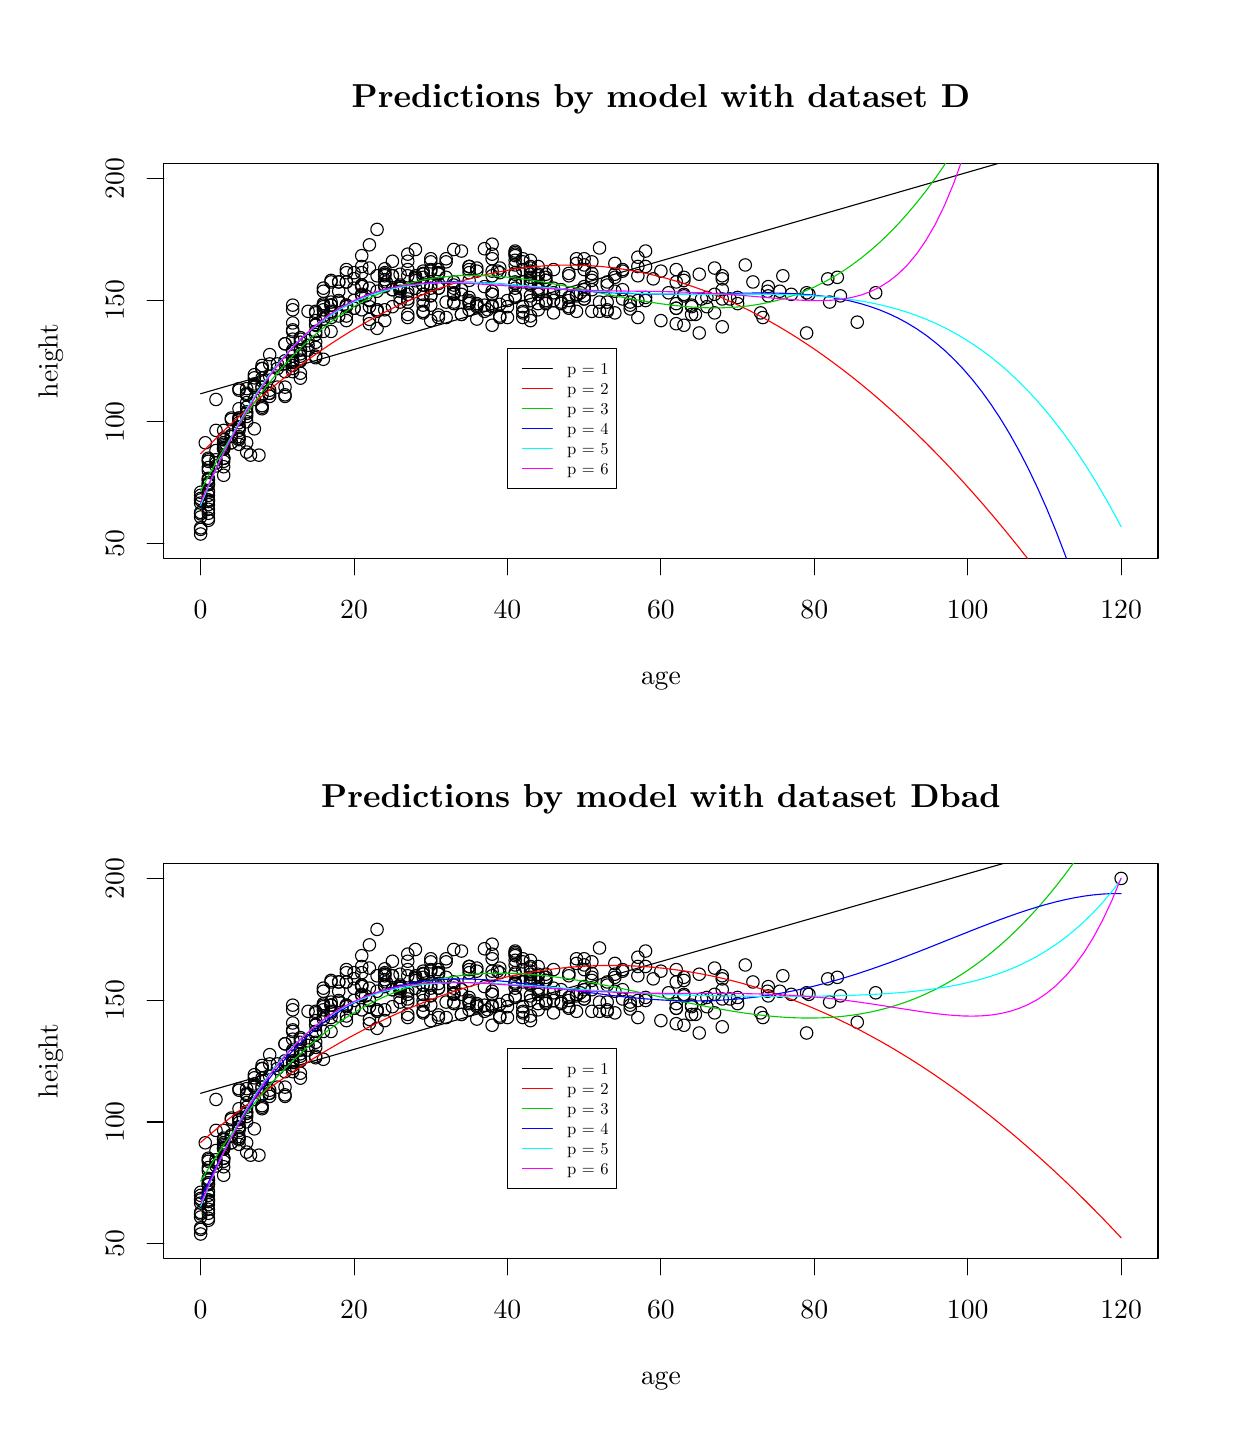
\begin{tikzpicture}[x=1pt,y=1pt]
\definecolor{fillColor}{RGB}{255,255,255}
\path[use as bounding box,fill=fillColor,fill opacity=0.00] (0,0) rectangle (433.62,505.89);
\begin{scope}
\path[clip] ( 49.20,314.14) rectangle (408.42,456.69);
\definecolor{drawColor}{RGB}{0,0,0}

\path[draw=drawColor,line width= 0.4pt,line join=round,line cap=round] (237.13,408.97) circle (  2.25);

\path[draw=drawColor,line width= 0.4pt,line join=round,line cap=round] (237.13,398.35) circle (  2.25);

\path[draw=drawColor,line width= 0.4pt,line join=round,line cap=round] (242.67,395.56) circle (  2.25);

\path[draw=drawColor,line width= 0.4pt,line join=round,line cap=round] (176.15,413.44) circle (  2.25);

\path[draw=drawColor,line width= 0.4pt,line join=round,line cap=round] (203.86,403.38) circle (  2.25);

\path[draw=drawColor,line width= 0.4pt,line join=round,line cap=round] (159.52,419.58) circle (  2.25);

\path[draw=drawColor,line width= 0.4pt,line join=round,line cap=round] (151.20,406.73) circle (  2.25);

\path[draw=drawColor,line width= 0.4pt,line join=round,line cap=round] (137.34,424.05) circle (  2.25);

\path[draw=drawColor,line width= 0.4pt,line join=round,line cap=round] (115.17,405.62) circle (  2.25);

\path[draw=drawColor,line width= 0.4pt,line join=round,line cap=round] (212.18,420.70) circle (  2.25);

\path[draw=drawColor,line width= 0.4pt,line join=round,line cap=round] (192.78,411.20) circle (  2.25);

\path[draw=drawColor,line width= 0.4pt,line join=round,line cap=round] (245.44,408.41) circle (  2.25);

\path[draw=drawColor,line width= 0.4pt,line join=round,line cap=round] (264.84,402.82) circle (  2.25);

\path[draw=drawColor,line width= 0.4pt,line join=round,line cap=round] (117.94,407.33) circle (  2.25);

\path[draw=drawColor,line width= 0.4pt,line join=round,line cap=round] (243.50,407.85) circle (  2.25);

\path[draw=drawColor,line width= 0.4pt,line join=round,line cap=round] (162.29,419.03) circle (  2.25);

\path[draw=drawColor,line width= 0.4pt,line join=round,line cap=round] (184.46,414.00) circle (  2.25);

\path[draw=drawColor,line width= 0.4pt,line join=round,line cap=round] (148.43,402.08) circle (  2.25);

\path[draw=drawColor,line width= 0.4pt,line join=round,line cap=round] ( 95.77,382.71) circle (  2.25);

\path[draw=drawColor,line width= 0.4pt,line join=round,line cap=round] ( 84.68,368.18) circle (  2.25);

\path[draw=drawColor,line width= 0.4pt,line join=round,line cap=round] ( 80.52,351.42) circle (  2.25);

\path[draw=drawColor,line width= 0.4pt,line join=round,line cap=round] (170.60,417.35) circle (  2.25);

\path[draw=drawColor,line width= 0.4pt,line join=round,line cap=round] (142.89,412.88) circle (  2.25);

\path[draw=drawColor,line width= 0.4pt,line join=round,line cap=round] ( 98.54,389.41) circle (  2.25);

\path[draw=drawColor,line width= 0.4pt,line join=round,line cap=round] ( 81.91,371.53) circle (  2.25);

\path[draw=drawColor,line width= 0.4pt,line join=round,line cap=round] (217.72,404.25) circle (  2.25);

\path[draw=drawColor,line width= 0.4pt,line join=round,line cap=round] (187.23,406.17) circle (  2.25);

\path[draw=drawColor,line width= 0.4pt,line join=round,line cap=round] (115.17,405.06) circle (  2.25);

\path[draw=drawColor,line width= 0.4pt,line join=round,line cap=round] (109.62,396.12) circle (  2.25);

\path[draw=drawColor,line width= 0.4pt,line join=round,line cap=round] (106.85,386.06) circle (  2.25);

\path[draw=drawColor,line width= 0.4pt,line join=round,line cap=round] ( 92.99,376.00) circle (  2.25);

\path[draw=drawColor,line width= 0.4pt,line join=round,line cap=round] (142.89,405.62) circle (  2.25);

\path[draw=drawColor,line width= 0.4pt,line join=round,line cap=round] (145.66,417.91) circle (  2.25);

\path[draw=drawColor,line width= 0.4pt,line join=round,line cap=round] (129.03,403.94) circle (  2.25);

\path[draw=drawColor,line width= 0.4pt,line join=round,line cap=round] (159.52,403.94) circle (  2.25);

\path[draw=drawColor,line width= 0.4pt,line join=round,line cap=round] (153.97,409.80) circle (  2.25);

\path[draw=drawColor,line width= 0.4pt,line join=round,line cap=round] (137.34,401.15) circle (  2.25);

\path[draw=drawColor,line width= 0.4pt,line join=round,line cap=round] (151.20,401.15) circle (  2.25);

\path[draw=drawColor,line width= 0.4pt,line join=round,line cap=round] (162.29,405.62) circle (  2.25);

\path[draw=drawColor,line width= 0.4pt,line join=round,line cap=round] (129.03,416.79) circle (  2.25);

\path[draw=drawColor,line width= 0.4pt,line join=round,line cap=round] (145.66,408.97) circle (  2.25);

\path[draw=drawColor,line width= 0.4pt,line join=round,line cap=round] (129.03,418.74) circle (  2.25);

\path[draw=drawColor,line width= 0.4pt,line join=round,line cap=round] (206.64,426.29) circle (  2.25);

\path[draw=drawColor,line width= 0.4pt,line join=round,line cap=round] (178.92,405.06) circle (  2.25);

\path[draw=drawColor,line width= 0.4pt,line join=round,line cap=round] (115.17,405.62) circle (  2.25);

\path[draw=drawColor,line width= 0.4pt,line join=round,line cap=round] (109.62,402.82) circle (  2.25);

\path[draw=drawColor,line width= 0.4pt,line join=round,line cap=round] ( 84.68,382.71) circle (  2.25);

\path[draw=drawColor,line width= 0.4pt,line join=round,line cap=round] ( 95.77,388.85) circle (  2.25);

\path[draw=drawColor,line width= 0.4pt,line join=round,line cap=round] ( 76.36,361.48) circle (  2.25);

\path[draw=drawColor,line width= 0.4pt,line join=round,line cap=round] (214.95,411.20) circle (  2.25);

\path[draw=drawColor,line width= 0.4pt,line join=round,line cap=round] (181.69,401.70) circle (  2.25);

\path[draw=drawColor,line width= 0.4pt,line join=round,line cap=round] (117.94,404.51) circle (  2.25);

\path[draw=drawColor,line width= 0.4pt,line join=round,line cap=round] (112.40,414.00) circle (  2.25);

\path[draw=drawColor,line width= 0.4pt,line join=round,line cap=round] ( 98.54,387.18) circle (  2.25);

\path[draw=drawColor,line width= 0.4pt,line join=round,line cap=round] ( 87.45,372.65) circle (  2.25);

\path[draw=drawColor,line width= 0.4pt,line join=round,line cap=round] ( 76.36,361.48) circle (  2.25);

\path[draw=drawColor,line width= 0.4pt,line join=round,line cap=round] (178.92,421.26) circle (  2.25);

\path[draw=drawColor,line width= 0.4pt,line join=round,line cap=round] (184.46,409.53) circle (  2.25);

\path[draw=drawColor,line width= 0.4pt,line join=round,line cap=round] (228.81,400.03) circle (  2.25);

\path[draw=drawColor,line width= 0.4pt,line join=round,line cap=round] (117.94,415.16) circle (  2.25);

\path[draw=drawColor,line width= 0.4pt,line join=round,line cap=round] (165.06,412.32) circle (  2.25);

\path[draw=drawColor,line width= 0.4pt,line join=round,line cap=round] (201.09,420.14) circle (  2.25);

\path[draw=drawColor,line width= 0.4pt,line join=round,line cap=round] (201.09,408.97) circle (  2.25);

\path[draw=drawColor,line width= 0.4pt,line join=round,line cap=round] (148.43,417.35) circle (  2.25);

\path[draw=drawColor,line width= 0.4pt,line join=round,line cap=round] (131.80,411.20) circle (  2.25);

\path[draw=drawColor,line width= 0.4pt,line join=round,line cap=round] (126.25,403.38) circle (  2.25);

\path[draw=drawColor,line width= 0.4pt,line join=round,line cap=round] (206.64,403.38) circle (  2.25);

\path[draw=drawColor,line width= 0.4pt,line join=round,line cap=round] (282.30,409.53) circle (  2.25);

\path[draw=drawColor,line width= 0.4pt,line join=round,line cap=round] (159.52,419.58) circle (  2.25);

\path[draw=drawColor,line width= 0.4pt,line join=round,line cap=round] (137.34,402.26) circle (  2.25);

\path[draw=drawColor,line width= 0.4pt,line join=round,line cap=round] ( 98.54,389.41) circle (  2.25);

\path[draw=drawColor,line width= 0.4pt,line join=round,line cap=round] (101.31,389.41) circle (  2.25);

\path[draw=drawColor,line width= 0.4pt,line join=round,line cap=round] (167.83,410.64) circle (  2.25);

\path[draw=drawColor,line width= 0.4pt,line join=round,line cap=round] (170.60,401.15) circle (  2.25);

\path[draw=drawColor,line width= 0.4pt,line join=round,line cap=round] ( 95.77,403.94) circle (  2.25);

\path[draw=drawColor,line width= 0.4pt,line join=round,line cap=round] (145.66,422.38) circle (  2.25);

\path[draw=drawColor,line width= 0.4pt,line join=round,line cap=round] (129.03,414.82) circle (  2.25);

\path[draw=drawColor,line width= 0.4pt,line join=round,line cap=round] ( 64.17,355.89) circle (  2.25);

\path[draw=drawColor,line width= 0.4pt,line join=round,line cap=round] (203.86,421.26) circle (  2.25);

\path[draw=drawColor,line width= 0.4pt,line join=round,line cap=round] (190.01,407.29) circle (  2.25);

\path[draw=drawColor,line width= 0.4pt,line join=round,line cap=round] (109.62,405.62) circle (  2.25);

\path[draw=drawColor,line width= 0.4pt,line join=round,line cap=round] ( 95.77,396.68) circle (  2.25);

\path[draw=drawColor,line width= 0.4pt,line join=round,line cap=round] (123.48,411.76) circle (  2.25);

\path[draw=drawColor,line width= 0.4pt,line join=round,line cap=round] (142.89,417.06) circle (  2.25);

\path[draw=drawColor,line width= 0.4pt,line join=round,line cap=round] (167.83,417.91) circle (  2.25);

\path[draw=drawColor,line width= 0.4pt,line join=round,line cap=round] (145.66,405.62) circle (  2.25);

\path[draw=drawColor,line width= 0.4pt,line join=round,line cap=round] ( 79.13,375.44) circle (  2.25);

\path[draw=drawColor,line width= 0.4pt,line join=round,line cap=round] (187.23,415.67) circle (  2.25);

\path[draw=drawColor,line width= 0.4pt,line join=round,line cap=round] (192.78,406.17) circle (  2.25);

\path[draw=drawColor,line width= 0.4pt,line join=round,line cap=round] (281.47,395.56) circle (  2.25);

\path[draw=drawColor,line width= 0.4pt,line join=round,line cap=round] (187.23,414.56) circle (  2.25);

\path[draw=drawColor,line width= 0.4pt,line join=round,line cap=round] (212.18,402.82) circle (  2.25);

\path[draw=drawColor,line width= 0.4pt,line join=round,line cap=round] (148.43,413.44) circle (  2.25);

\path[draw=drawColor,line width= 0.4pt,line join=round,line cap=round] (126.25,432.99) circle (  2.25);

\path[draw=drawColor,line width= 0.4pt,line join=round,line cap=round] ( 87.45,379.91) circle (  2.25);

\path[draw=drawColor,line width= 0.4pt,line join=round,line cap=round] (176.15,425.17) circle (  2.25);

\path[draw=drawColor,line width= 0.4pt,line join=round,line cap=round] (126.25,403.94) circle (  2.25);

\path[draw=drawColor,line width= 0.4pt,line join=round,line cap=round] (162.29,405.06) circle (  2.25);

\path[draw=drawColor,line width= 0.4pt,line join=round,line cap=round] ( 76.36,374.89) circle (  2.25);

\path[draw=drawColor,line width= 0.4pt,line join=round,line cap=round] (145.66,418.47) circle (  2.25);

\path[draw=drawColor,line width= 0.4pt,line join=round,line cap=round] ( 95.77,393.32) circle (  2.25);

\path[draw=drawColor,line width= 0.4pt,line join=round,line cap=round] (156.74,409.53) circle (  2.25);

\path[draw=drawColor,line width= 0.4pt,line join=round,line cap=round] (184.46,416.23) circle (  2.25);

\path[draw=drawColor,line width= 0.4pt,line join=round,line cap=round] (181.69,407.29) circle (  2.25);

\path[draw=drawColor,line width= 0.4pt,line join=round,line cap=round] (265.67,401.15) circle (  2.25);

\path[draw=drawColor,line width= 0.4pt,line join=round,line cap=round] (167.83,422.38) circle (  2.25);

\path[draw=drawColor,line width= 0.4pt,line join=round,line cap=round] (181.69,415.67) circle (  2.25);

\path[draw=drawColor,line width= 0.4pt,line join=round,line cap=round] (153.97,411.76) circle (  2.25);

\path[draw=drawColor,line width= 0.4pt,line join=round,line cap=round] (106.85,406.17) circle (  2.25);

\path[draw=drawColor,line width= 0.4pt,line join=round,line cap=round] ( 92.99,373.21) circle (  2.25);

\path[draw=drawColor,line width= 0.4pt,line join=round,line cap=round] ( 79.13,373.77) circle (  2.25);

\path[draw=drawColor,line width= 0.4pt,line join=round,line cap=round] (159.52,418.47) circle (  2.25);

\path[draw=drawColor,line width= 0.4pt,line join=round,line cap=round] (142.89,409.53) circle (  2.25);

\path[draw=drawColor,line width= 0.4pt,line join=round,line cap=round] ( 95.77,384.94) circle (  2.25);

\path[draw=drawColor,line width= 0.4pt,line join=round,line cap=round] ( 87.45,373.77) circle (  2.25);

\path[draw=drawColor,line width= 0.4pt,line join=round,line cap=round] ( 83.57,351.42) circle (  2.25);

\path[draw=drawColor,line width= 0.4pt,line join=round,line cap=round] (223.27,425.17) circle (  2.25);

\path[draw=drawColor,line width= 0.4pt,line join=round,line cap=round] (209.41,403.94) circle (  2.25);

\path[draw=drawColor,line width= 0.4pt,line join=round,line cap=round] (203.86,415.67) circle (  2.25);

\path[draw=drawColor,line width= 0.4pt,line join=round,line cap=round] (195.55,408.41) circle (  2.25);

\path[draw=drawColor,line width= 0.4pt,line join=round,line cap=round] (142.89,416.79) circle (  2.25);

\path[draw=drawColor,line width= 0.4pt,line join=round,line cap=round] (176.15,424.61) circle (  2.25);

\path[draw=drawColor,line width= 0.4pt,line join=round,line cap=round] (289.10,415.11) circle (  2.25);

\path[draw=drawColor,line width= 0.4pt,line join=round,line cap=round] ( 65.28,340.80) circle (  2.25);

\path[draw=drawColor,line width= 0.4pt,line join=round,line cap=round] (159.52,407.29) circle (  2.25);

\path[draw=drawColor,line width= 0.4pt,line join=round,line cap=round] (190.01,410.09) circle (  2.25);

\path[draw=drawColor,line width= 0.4pt,line join=round,line cap=round] ( 76.36,360.36) circle (  2.25);

\path[draw=drawColor,line width= 0.4pt,line join=round,line cap=round] (142.89,417.91) circle (  2.25);

\path[draw=drawColor,line width= 0.4pt,line join=round,line cap=round] (178.92,418.47) circle (  2.25);

\path[draw=drawColor,line width= 0.4pt,line join=round,line cap=round] (137.34,406.73) circle (  2.25);

\path[draw=drawColor,line width= 0.4pt,line join=round,line cap=round] ( 84.68,378.24) circle (  2.25);

\path[draw=drawColor,line width= 0.4pt,line join=round,line cap=round] ( 79.13,363.49) circle (  2.25);

\path[draw=drawColor,line width= 0.4pt,line join=round,line cap=round] (123.48,419.03) circle (  2.25);

\path[draw=drawColor,line width= 0.4pt,line join=round,line cap=round] (181.69,417.91) circle (  2.25);

\path[draw=drawColor,line width= 0.4pt,line join=round,line cap=round] (209.41,403.38) circle (  2.25);

\path[draw=drawColor,line width= 0.4pt,line join=round,line cap=round] (181.69,419.03) circle (  2.25);

\path[draw=drawColor,line width= 0.4pt,line join=round,line cap=round] (176.15,408.41) circle (  2.25);

\path[draw=drawColor,line width= 0.4pt,line join=round,line cap=round] (201.09,407.85) circle (  2.25);

\path[draw=drawColor,line width= 0.4pt,line join=round,line cap=round] (104.08,400.03) circle (  2.25);

\path[draw=drawColor,line width= 0.4pt,line join=round,line cap=round] (153.97,425.73) circle (  2.25);

\path[draw=drawColor,line width= 0.4pt,line join=round,line cap=round] ( 70.82,355.89) circle (  2.25);

\path[draw=drawColor,line width= 0.4pt,line join=round,line cap=round] (234.35,414.00) circle (  2.25);

\path[draw=drawColor,line width= 0.4pt,line join=round,line cap=round] (198.32,409.53) circle (  2.25);

\path[draw=drawColor,line width= 0.4pt,line join=round,line cap=round] (109.62,406.73) circle (  2.25);

\path[draw=drawColor,line width= 0.4pt,line join=round,line cap=round] ( 95.77,389.41) circle (  2.25);

\path[draw=drawColor,line width= 0.4pt,line join=round,line cap=round] (123.48,405.06) circle (  2.25);

\path[draw=drawColor,line width= 0.4pt,line join=round,line cap=round] (142.89,403.38) circle (  2.25);

\path[draw=drawColor,line width= 0.4pt,line join=round,line cap=round] ( 84.68,382.71) circle (  2.25);

\path[draw=drawColor,line width= 0.4pt,line join=round,line cap=round] ( 76.36,375.44) circle (  2.25);

\path[draw=drawColor,line width= 0.4pt,line join=round,line cap=round] (153.97,414.00) circle (  2.25);

\path[draw=drawColor,line width= 0.4pt,line join=round,line cap=round] (156.74,411.20) circle (  2.25);

\path[draw=drawColor,line width= 0.4pt,line join=round,line cap=round] ( 95.77,381.59) circle (  2.25);

\path[draw=drawColor,line width= 0.4pt,line join=round,line cap=round] ( 81.91,377.15) circle (  2.25);

\path[draw=drawColor,line width= 0.4pt,line join=round,line cap=round] (178.92,422.38) circle (  2.25);

\path[draw=drawColor,line width= 0.4pt,line join=round,line cap=round] (173.37,401.15) circle (  2.25);

\path[draw=drawColor,line width= 0.4pt,line join=round,line cap=round] (137.34,409.53) circle (  2.25);

\path[draw=drawColor,line width= 0.4pt,line join=round,line cap=round] ( 70.82,360.36) circle (  2.25);

\path[draw=drawColor,line width= 0.4pt,line join=round,line cap=round] (131.80,416.21) circle (  2.25);

\path[draw=drawColor,line width= 0.4pt,line join=round,line cap=round] (142.89,415.67) circle (  2.25);

\path[draw=drawColor,line width= 0.4pt,line join=round,line cap=round] (187.23,407.29) circle (  2.25);

\path[draw=drawColor,line width= 0.4pt,line join=round,line cap=round] (134.57,416.79) circle (  2.25);

\path[draw=drawColor,line width= 0.4pt,line join=round,line cap=round] (187.23,416.79) circle (  2.25);

\path[draw=drawColor,line width= 0.4pt,line join=round,line cap=round] (187.23,406.73) circle (  2.25);

\path[draw=drawColor,line width= 0.4pt,line join=round,line cap=round] ( 92.99,385.50) circle (  2.25);

\path[draw=drawColor,line width= 0.4pt,line join=round,line cap=round] (299.77,399.47) circle (  2.25);

\path[draw=drawColor,line width= 0.4pt,line join=round,line cap=round] (134.57,411.76) circle (  2.25);

\path[draw=drawColor,line width= 0.4pt,line join=round,line cap=round] (129.03,400.03) circle (  2.25);

\path[draw=drawColor,line width= 0.4pt,line join=round,line cap=round] (220.49,416.23) circle (  2.25);

\path[draw=drawColor,line width= 0.4pt,line join=round,line cap=round] (123.48,407.56) circle (  2.25);

\path[draw=drawColor,line width= 0.4pt,line join=round,line cap=round] (129.03,412.32) circle (  2.25);

\path[draw=drawColor,line width= 0.4pt,line join=round,line cap=round] ( 79.13,366.50) circle (  2.25);

\path[draw=drawColor,line width= 0.4pt,line join=round,line cap=round] ( 73.59,358.68) circle (  2.25);

\path[draw=drawColor,line width= 0.4pt,line join=round,line cap=round] (120.71,412.88) circle (  2.25);

\path[draw=drawColor,line width= 0.4pt,line join=round,line cap=round] (281.47,410.09) circle (  2.25);

\path[draw=drawColor,line width= 0.4pt,line join=round,line cap=round] (201.09,422.38) circle (  2.25);

\path[draw=drawColor,line width= 0.4pt,line join=round,line cap=round] (173.37,407.29) circle (  2.25);

\path[draw=drawColor,line width= 0.4pt,line join=round,line cap=round] (239.90,405.62) circle (  2.25);

\path[draw=drawColor,line width= 0.4pt,line join=round,line cap=round] (151.20,415.67) circle (  2.25);

\path[draw=drawColor,line width= 0.4pt,line join=round,line cap=round] (169.77,417.91) circle (  2.25);

\path[draw=drawColor,line width= 0.4pt,line join=round,line cap=round] (134.57,412.32) circle (  2.25);

\path[draw=drawColor,line width= 0.4pt,line join=round,line cap=round] (237.13,415.67) circle (  2.25);

\path[draw=drawColor,line width= 0.4pt,line join=round,line cap=round] (234.35,404.50) circle (  2.25);

\path[draw=drawColor,line width= 0.4pt,line join=round,line cap=round] (123.48,427.41) circle (  2.25);

\path[draw=drawColor,line width= 0.4pt,line join=round,line cap=round] (176.15,421.82) circle (  2.25);

\path[draw=drawColor,line width= 0.4pt,line join=round,line cap=round] (115.17,400.03) circle (  2.25);

\path[draw=drawColor,line width= 0.4pt,line join=round,line cap=round] (109.62,401.15) circle (  2.25);

\path[draw=drawColor,line width= 0.4pt,line join=round,line cap=round] (101.31,392.76) circle (  2.25);

\path[draw=drawColor,line width= 0.4pt,line join=round,line cap=round] ( 87.45,387.74) circle (  2.25);

\path[draw=drawColor,line width= 0.4pt,line join=round,line cap=round] ( 81.91,380.47) circle (  2.25);

\path[draw=drawColor,line width= 0.4pt,line join=round,line cap=round] (267.61,408.97) circle (  2.25);

\path[draw=drawColor,line width= 0.4pt,line join=round,line cap=round] (176.15,413.44) circle (  2.25);

\path[draw=drawColor,line width= 0.4pt,line join=round,line cap=round] (153.97,406.17) circle (  2.25);

\path[draw=drawColor,line width= 0.4pt,line join=round,line cap=round] (209.41,414.00) circle (  2.25);

\path[draw=drawColor,line width= 0.4pt,line join=round,line cap=round] (112.40,407.29) circle (  2.25);

\path[draw=drawColor,line width= 0.4pt,line join=round,line cap=round] (165.06,405.62) circle (  2.25);

\path[draw=drawColor,line width= 0.4pt,line join=round,line cap=round] ( 79.13,365.39) circle (  2.25);

\path[draw=drawColor,line width= 0.4pt,line join=round,line cap=round] (231.58,410.09) circle (  2.25);

\path[draw=drawColor,line width= 0.4pt,line join=round,line cap=round] (184.46,416.79) circle (  2.25);

\path[draw=drawColor,line width= 0.4pt,line join=round,line cap=round] (159.52,406.73) circle (  2.25);

\path[draw=drawColor,line width= 0.4pt,line join=round,line cap=round] ( 81.91,376.00) circle (  2.25);

\path[draw=drawColor,line width= 0.4pt,line join=round,line cap=round] ( 73.59,364.27) circle (  2.25);

\path[draw=drawColor,line width= 0.4pt,line join=round,line cap=round] (126.25,397.23) circle (  2.25);

\path[draw=drawColor,line width= 0.4pt,line join=round,line cap=round] ( 73.59,355.89) circle (  2.25);

\path[draw=drawColor,line width= 0.4pt,line join=round,line cap=round] (214.95,418.47) circle (  2.25);

\path[draw=drawColor,line width= 0.4pt,line join=round,line cap=round] (209.41,406.73) circle (  2.25);

\path[draw=drawColor,line width= 0.4pt,line join=round,line cap=round] (226.04,415.11) circle (  2.25);

\path[draw=drawColor,line width= 0.4pt,line join=round,line cap=round] (220.49,407.29) circle (  2.25);

\path[draw=drawColor,line width= 0.4pt,line join=round,line cap=round] (159.52,414.56) circle (  2.25);

\path[draw=drawColor,line width= 0.4pt,line join=round,line cap=round] (142.89,412.88) circle (  2.25);

\path[draw=drawColor,line width= 0.4pt,line join=round,line cap=round] (234.35,406.17) circle (  2.25);

\path[draw=drawColor,line width= 0.4pt,line join=round,line cap=round] (112.40,401.70) circle (  2.25);

\path[draw=drawColor,line width= 0.4pt,line join=round,line cap=round] (203.86,411.20) circle (  2.25);

\path[draw=drawColor,line width= 0.4pt,line join=round,line cap=round] (101.31,391.09) circle (  2.25);

\path[draw=drawColor,line width= 0.4pt,line join=round,line cap=round] (115.17,414.00) circle (  2.25);

\path[draw=drawColor,line width= 0.4pt,line join=round,line cap=round] (178.92,414.00) circle (  2.25);

\path[draw=drawColor,line width= 0.4pt,line join=round,line cap=round] (131.80,411.20) circle (  2.25);

\path[draw=drawColor,line width= 0.4pt,line join=round,line cap=round] ( 79.13,370.42) circle (  2.25);

\path[draw=drawColor,line width= 0.4pt,line join=round,line cap=round] (176.15,423.50) circle (  2.25);

\path[draw=drawColor,line width= 0.4pt,line join=round,line cap=round] (165.06,403.38) circle (  2.25);

\path[draw=drawColor,line width= 0.4pt,line join=round,line cap=round] (106.85,405.62) circle (  2.25);

\path[draw=drawColor,line width= 0.4pt,line join=round,line cap=round] ( 76.36,364.27) circle (  2.25);

\path[draw=drawColor,line width= 0.4pt,line join=round,line cap=round] ( 87.45,374.89) circle (  2.25);

\path[draw=drawColor,line width= 0.4pt,line join=round,line cap=round] (289.79,406.73) circle (  2.25);

\path[draw=drawColor,line width= 0.4pt,line join=round,line cap=round] (140.11,411.76) circle (  2.25);

\path[draw=drawColor,line width= 0.4pt,line join=round,line cap=round] (201.09,418.47) circle (  2.25);

\path[draw=drawColor,line width= 0.4pt,line join=round,line cap=round] (181.69,413.44) circle (  2.25);

\path[draw=drawColor,line width= 0.4pt,line join=round,line cap=round] ( 84.68,383.82) circle (  2.25);

\path[draw=drawColor,line width= 0.4pt,line join=round,line cap=round] (148.43,417.10) circle (  2.25);

\path[draw=drawColor,line width= 0.4pt,line join=round,line cap=round] (248.21,402.82) circle (  2.25);

\path[draw=drawColor,line width= 0.4pt,line join=round,line cap=round] (170.60,401.70) circle (  2.25);

\path[draw=drawColor,line width= 0.4pt,line join=round,line cap=round] (112.40,406.73) circle (  2.25);

\path[draw=drawColor,line width= 0.4pt,line join=round,line cap=round] ( 92.99,372.65) circle (  2.25);

\path[draw=drawColor,line width= 0.4pt,line join=round,line cap=round] (195.55,407.29) circle (  2.25);

\path[draw=drawColor,line width= 0.4pt,line join=round,line cap=round] (145.66,421.26) circle (  2.25);

\path[draw=drawColor,line width= 0.4pt,line join=round,line cap=round] (239.90,402.26) circle (  2.25);

\path[draw=drawColor,line width= 0.4pt,line join=round,line cap=round] (262.07,414.00) circle (  2.25);

\path[draw=drawColor,line width= 0.4pt,line join=round,line cap=round] (250.98,411.20) circle (  2.25);

\path[draw=drawColor,line width= 0.4pt,line join=round,line cap=round] (184.46,419.58) circle (  2.25);

\path[draw=drawColor,line width= 0.4pt,line join=round,line cap=round] (181.69,412.88) circle (  2.25);

\path[draw=drawColor,line width= 0.4pt,line join=round,line cap=round] (106.85,410.64) circle (  2.25);

\path[draw=drawColor,line width= 0.4pt,line join=round,line cap=round] ( 98.54,393.88) circle (  2.25);

\path[draw=drawColor,line width= 0.4pt,line join=round,line cap=round] (156.74,402.26) circle (  2.25);

\path[draw=drawColor,line width= 0.4pt,line join=round,line cap=round] ( 90.22,376.00) circle (  2.25);

\path[draw=drawColor,line width= 0.4pt,line join=round,line cap=round] (234.35,418.47) circle (  2.25);

\path[draw=drawColor,line width= 0.4pt,line join=round,line cap=round] (184.46,403.94) circle (  2.25);

\path[draw=drawColor,line width= 0.4pt,line join=round,line cap=round] ( 92.99,381.59) circle (  2.25);

\path[draw=drawColor,line width= 0.4pt,line join=round,line cap=round] (148.43,411.76) circle (  2.25);

\path[draw=drawColor,line width= 0.4pt,line join=round,line cap=round] (142.89,402.82) circle (  2.25);

\path[draw=drawColor,line width= 0.4pt,line join=round,line cap=round] ( 84.68,369.30) circle (  2.25);

\path[draw=drawColor,line width= 0.4pt,line join=round,line cap=round] (234.35,404.50) circle (  2.25);

\path[draw=drawColor,line width= 0.4pt,line join=round,line cap=round] (248.21,409.53) circle (  2.25);

\path[draw=drawColor,line width= 0.4pt,line join=round,line cap=round] (220.49,419.58) circle (  2.25);

\path[draw=drawColor,line width= 0.4pt,line join=round,line cap=round] (151.20,421.26) circle (  2.25);

\path[draw=drawColor,line width= 0.4pt,line join=round,line cap=round] (129.03,412.88) circle (  2.25);

\path[draw=drawColor,line width= 0.4pt,line join=round,line cap=round] (275.93,409.53) circle (  2.25);

\path[draw=drawColor,line width= 0.4pt,line join=round,line cap=round] (234.35,398.91) circle (  2.25);

\path[draw=drawColor,line width= 0.4pt,line join=round,line cap=round] (109.62,414.56) circle (  2.25);

\path[draw=drawColor,line width= 0.4pt,line join=round,line cap=round] (248.21,419.03) circle (  2.25);

\path[draw=drawColor,line width= 0.4pt,line join=round,line cap=round] (256.53,408.41) circle (  2.25);

\path[draw=drawColor,line width= 0.4pt,line join=round,line cap=round] (165.06,426.00) circle (  2.25);

\path[draw=drawColor,line width= 0.4pt,line join=round,line cap=round] (223.27,407.29) circle (  2.25);

\path[draw=drawColor,line width= 0.4pt,line join=round,line cap=round] (159.52,419.58) circle (  2.25);

\path[draw=drawColor,line width= 0.4pt,line join=round,line cap=round] (145.66,400.03) circle (  2.25);

\path[draw=drawColor,line width= 0.4pt,line join=round,line cap=round] ( 76.36,358.12) circle (  2.25);

\path[draw=drawColor,line width= 0.4pt,line join=round,line cap=round] (134.57,406.73) circle (  2.25);

\path[draw=drawColor,line width= 0.4pt,line join=round,line cap=round] ( 76.36,368.18) circle (  2.25);

\path[draw=drawColor,line width= 0.4pt,line join=round,line cap=round] (120.71,403.94) circle (  2.25);

\path[draw=drawColor,line width= 0.4pt,line join=round,line cap=round] (176.15,417.35) circle (  2.25);

\path[draw=drawColor,line width= 0.4pt,line join=round,line cap=round] (190.01,418.47) circle (  2.25);

\path[draw=drawColor,line width= 0.4pt,line join=round,line cap=round] (198.32,403.38) circle (  2.25);

\path[draw=drawColor,line width= 0.4pt,line join=round,line cap=round] (104.08,403.38) circle (  2.25);

\path[draw=drawColor,line width= 0.4pt,line join=round,line cap=round] (140.11,425.73) circle (  2.25);

\path[draw=drawColor,line width= 0.4pt,line join=round,line cap=round] ( 95.77,387.18) circle (  2.25);

\path[draw=drawColor,line width= 0.4pt,line join=round,line cap=round] (292.56,415.67) circle (  2.25);

\path[draw=drawColor,line width= 0.4pt,line join=round,line cap=round] (212.18,415.69) circle (  2.25);

\path[draw=drawColor,line width= 0.4pt,line join=round,line cap=round] (212.18,410.64) circle (  2.25);

\path[draw=drawColor,line width= 0.4pt,line join=round,line cap=round] (250.98,416.23) circle (  2.25);

\path[draw=drawColor,line width= 0.4pt,line join=round,line cap=round] (250.98,407.85) circle (  2.25);

\path[draw=drawColor,line width= 0.4pt,line join=round,line cap=round] (217.72,406.73) circle (  2.25);

\path[draw=drawColor,line width= 0.4pt,line join=round,line cap=round] (104.08,387.18) circle (  2.25);

\path[draw=drawColor,line width= 0.4pt,line join=round,line cap=round] (220.49,401.15) circle (  2.25);

\path[draw=drawColor,line width= 0.4pt,line join=round,line cap=round] (123.48,400.48) circle (  2.25);

\path[draw=drawColor,line width= 0.4pt,line join=round,line cap=round] (173.37,405.06) circle (  2.25);

\path[draw=drawColor,line width= 0.4pt,line join=round,line cap=round] (115.17,418.47) circle (  2.25);

\path[draw=drawColor,line width= 0.4pt,line join=round,line cap=round] (176.15,420.14) circle (  2.25);

\path[draw=drawColor,line width= 0.4pt,line join=round,line cap=round] (272.88,416.23) circle (  2.25);

\path[draw=drawColor,line width= 0.4pt,line join=round,line cap=round] (267.34,410.64) circle (  2.25);

\path[draw=drawColor,line width= 0.4pt,line join=round,line cap=round] (198.32,422.38) circle (  2.25);

\path[draw=drawColor,line width= 0.4pt,line join=round,line cap=round] (134.57,408.41) circle (  2.25);

\path[draw=drawColor,line width= 0.4pt,line join=round,line cap=round] (109.62,405.62) circle (  2.25);

\path[draw=drawColor,line width= 0.4pt,line join=round,line cap=round] ( 98.54,385.77) circle (  2.25);

\path[draw=drawColor,line width= 0.4pt,line join=round,line cap=round] ( 84.68,373.21) circle (  2.25);

\path[draw=drawColor,line width= 0.4pt,line join=round,line cap=round] (306.42,410.09) circle (  2.25);

\path[draw=drawColor,line width= 0.4pt,line join=round,line cap=round] (250.98,397.79) circle (  2.25);

\path[draw=drawColor,line width= 0.4pt,line join=round,line cap=round] (153.97,409.53) circle (  2.25);

\path[draw=drawColor,line width= 0.4pt,line join=round,line cap=round] (134.57,411.76) circle (  2.25);

\path[draw=drawColor,line width= 0.4pt,line join=round,line cap=round] (217.72,405.62) circle (  2.25);

\path[draw=drawColor,line width= 0.4pt,line join=round,line cap=round] (106.85,401.70) circle (  2.25);

\path[draw=drawColor,line width= 0.4pt,line join=round,line cap=round] ( 98.54,379.24) circle (  2.25);

\path[draw=drawColor,line width= 0.4pt,line join=round,line cap=round] (156.74,402.26) circle (  2.25);

\path[draw=drawColor,line width= 0.4pt,line join=round,line cap=round] ( 76.36,357.01) circle (  2.25);

\path[draw=drawColor,line width= 0.4pt,line join=round,line cap=round] (109.62,405.62) circle (  2.25);

\path[draw=drawColor,line width= 0.4pt,line join=round,line cap=round] (267.61,412.32) circle (  2.25);

\path[draw=drawColor,line width= 0.4pt,line join=round,line cap=round] (253.76,407.85) circle (  2.25);

\path[draw=drawColor,line width= 0.4pt,line join=round,line cap=round] (201.09,412.32) circle (  2.25);

\path[draw=drawColor,line width= 0.4pt,line join=round,line cap=round] (184.46,411.20) circle (  2.25);

\path[draw=drawColor,line width= 0.4pt,line join=round,line cap=round] (104.08,390.35) circle (  2.25);

\path[draw=drawColor,line width= 0.4pt,line join=round,line cap=round] ( 76.36,364.83) circle (  2.25);

\path[draw=drawColor,line width= 0.4pt,line join=round,line cap=round] (112.40,414.00) circle (  2.25);

\path[draw=drawColor,line width= 0.4pt,line join=round,line cap=round] (176.15,424.05) circle (  2.25);

\path[draw=drawColor,line width= 0.4pt,line join=round,line cap=round] (137.34,407.85) circle (  2.25);

\path[draw=drawColor,line width= 0.4pt,line join=round,line cap=round] ( 87.17,373.77) circle (  2.25);

\path[draw=drawColor,line width= 0.4pt,line join=round,line cap=round] (167.83,416.23) circle (  2.25);

\path[draw=drawColor,line width= 0.4pt,line join=round,line cap=round] (220.49,422.94) circle (  2.25);

\path[draw=drawColor,line width= 0.4pt,line join=round,line cap=round] (241.28,402.26) circle (  2.25);

\path[draw=drawColor,line width= 0.4pt,line join=round,line cap=round] (178.92,403.38) circle (  2.25);

\path[draw=drawColor,line width= 0.4pt,line join=round,line cap=round] (129.03,416.23) circle (  2.25);

\path[draw=drawColor,line width= 0.4pt,line join=round,line cap=round] (106.85,405.06) circle (  2.25);

\path[draw=drawColor,line width= 0.4pt,line join=round,line cap=round] (259.30,420.14) circle (  2.25);

\path[draw=drawColor,line width= 0.4pt,line join=round,line cap=round] (199.71,410.09) circle (  2.25);

\path[draw=drawColor,line width= 0.4pt,line join=round,line cap=round] (153.97,406.73) circle (  2.25);

\path[draw=drawColor,line width= 0.4pt,line join=round,line cap=round] (140.11,416.23) circle (  2.25);

\path[draw=drawColor,line width= 0.4pt,line join=round,line cap=round] (192.78,406.73) circle (  2.25);

\path[draw=drawColor,line width= 0.4pt,line join=round,line cap=round] ( 70.82,350.30) circle (  2.25);

\path[draw=drawColor,line width= 0.4pt,line join=round,line cap=round] ( 65.28,349.74) circle (  2.25);

\path[draw=drawColor,line width= 0.4pt,line join=round,line cap=round] ( 65.28,327.88) circle (  2.25);

\path[draw=drawColor,line width= 0.4pt,line join=round,line cap=round] ( 70.82,357.01) circle (  2.25);

\path[draw=drawColor,line width= 0.4pt,line join=round,line cap=round] ( 79.13,373.21) circle (  2.25);

\path[draw=drawColor,line width= 0.4pt,line join=round,line cap=round] ( 76.36,355.33) circle (  2.25);

\path[draw=drawColor,line width= 0.4pt,line join=round,line cap=round] (137.34,410.64) circle (  2.25);

\path[draw=drawColor,line width= 0.4pt,line join=round,line cap=round] ( 76.36,363.15) circle (  2.25);

\path[draw=drawColor,line width= 0.4pt,line join=round,line cap=round] ( 65.28,330.41) circle (  2.25);

\path[draw=drawColor,line width= 0.4pt,line join=round,line cap=round] ( 68.05,347.51) circle (  2.25);

\path[draw=drawColor,line width= 0.4pt,line join=round,line cap=round] ( 68.05,360.36) circle (  2.25);

\path[draw=drawColor,line width= 0.4pt,line join=round,line cap=round] ( 65.28,345.83) circle (  2.25);

\path[draw=drawColor,line width= 0.4pt,line join=round,line cap=round] (214.95,407.85) circle (  2.25);

\path[draw=drawColor,line width= 0.4pt,line join=round,line cap=round] (293.67,408.97) circle (  2.25);

\path[draw=drawColor,line width= 0.4pt,line join=round,line cap=round] ( 95.77,399.18) circle (  2.25);

\path[draw=drawColor,line width= 0.4pt,line join=round,line cap=round] ( 68.05,353.09) circle (  2.25);

\path[draw=drawColor,line width= 0.4pt,line join=round,line cap=round] (237.13,414.56) circle (  2.25);

\path[draw=drawColor,line width= 0.4pt,line join=round,line cap=round] (206.64,406.73) circle (  2.25);

\path[draw=drawColor,line width= 0.4pt,line join=round,line cap=round] (198.32,408.97) circle (  2.25);

\path[draw=drawColor,line width= 0.4pt,line join=round,line cap=round] (148.43,411.76) circle (  2.25);

\path[draw=drawColor,line width= 0.4pt,line join=round,line cap=round] ( 87.45,384.38) circle (  2.25);

\path[draw=drawColor,line width= 0.4pt,line join=round,line cap=round] ( 79.13,367.06) circle (  2.25);

\path[draw=drawColor,line width= 0.4pt,line join=round,line cap=round] (159.52,417.35) circle (  2.25);

\path[draw=drawColor,line width= 0.4pt,line join=round,line cap=round] (159.52,406.17) circle (  2.25);

\path[draw=drawColor,line width= 0.4pt,line join=round,line cap=round] ( 81.91,360.92) circle (  2.25);

\path[draw=drawColor,line width= 0.4pt,line join=round,line cap=round] ( 76.36,357.56) circle (  2.25);

\path[draw=drawColor,line width= 0.4pt,line join=round,line cap=round] (129.03,416.79) circle (  2.25);

\path[draw=drawColor,line width= 0.4pt,line join=round,line cap=round] (176.15,414.00) circle (  2.25);

\path[draw=drawColor,line width= 0.4pt,line join=round,line cap=round] (151.20,422.38) circle (  2.25);

\path[draw=drawColor,line width= 0.4pt,line join=round,line cap=round] (181.69,414.00) circle (  2.25);

\path[draw=drawColor,line width= 0.4pt,line join=round,line cap=round] ( 79.13,355.89) circle (  2.25);

\path[draw=drawColor,line width= 0.4pt,line join=round,line cap=round] ( 65.28,328.62) circle (  2.25);

\path[draw=drawColor,line width= 0.4pt,line join=round,line cap=round] (104.08,396.12) circle (  2.25);

\path[draw=drawColor,line width= 0.4pt,line join=round,line cap=round] (237.13,409.53) circle (  2.25);

\path[draw=drawColor,line width= 0.4pt,line join=round,line cap=round] (120.71,409.53) circle (  2.25);

\path[draw=drawColor,line width= 0.4pt,line join=round,line cap=round] ( 65.28,346.95) circle (  2.25);

\path[draw=drawColor,line width= 0.4pt,line join=round,line cap=round] ( 68.05,371.53) circle (  2.25);

\path[draw=drawColor,line width= 0.4pt,line join=round,line cap=round] ( 65.28,338.01) circle (  2.25);

\path[draw=drawColor,line width= 0.4pt,line join=round,line cap=round] ( 70.82,353.92) circle (  2.25);

\path[draw=drawColor,line width= 0.4pt,line join=round,line cap=round] ( 65.28,334.66) circle (  2.25);

\path[draw=drawColor,line width= 0.4pt,line join=round,line cap=round] ( 65.28,350.30) circle (  2.25);

\path[draw=drawColor,line width= 0.4pt,line join=round,line cap=round] ( 65.28,336.89) circle (  2.25);

\path[draw=drawColor,line width= 0.4pt,line join=round,line cap=round] (214.95,417.91) circle (  2.25);

\path[draw=drawColor,line width= 0.4pt,line join=round,line cap=round] (167.83,409.53) circle (  2.25);

\path[draw=drawColor,line width= 0.4pt,line join=round,line cap=round] ( 70.82,353.65) circle (  2.25);

\path[draw=drawColor,line width= 0.4pt,line join=round,line cap=round] ( 70.82,354.77) circle (  2.25);

\path[draw=drawColor,line width= 0.4pt,line join=round,line cap=round] ( 65.28,338.57) circle (  2.25);

\path[draw=drawColor,line width= 0.4pt,line join=round,line cap=round] ( 65.28,349.18) circle (  2.25);

\path[draw=drawColor,line width= 0.4pt,line join=round,line cap=round] (140.11,415.67) circle (  2.25);

\path[draw=drawColor,line width= 0.4pt,line join=round,line cap=round] (106.85,400.59) circle (  2.25);

\path[draw=drawColor,line width= 0.4pt,line join=round,line cap=round] (162.29,400.59) circle (  2.25);

\path[draw=drawColor,line width= 0.4pt,line join=round,line cap=round] (167.83,424.05) circle (  2.25);

\path[draw=drawColor,line width= 0.4pt,line join=round,line cap=round] ( 95.77,383.82) circle (  2.25);

\path[draw=drawColor,line width= 0.4pt,line join=round,line cap=round] ( 65.28,341.36) circle (  2.25);

\path[draw=drawColor,line width= 0.4pt,line join=round,line cap=round] ( 65.28,340.80) circle (  2.25);

\path[draw=drawColor,line width= 0.4pt,line join=round,line cap=round] ( 70.82,355.33) circle (  2.25);

\path[draw=drawColor,line width= 0.4pt,line join=round,line cap=round] (195.55,416.23) circle (  2.25);

\path[draw=drawColor,line width= 0.4pt,line join=round,line cap=round] ( 65.28,335.21) circle (  2.25);

\path[draw=drawColor,line width= 0.4pt,line join=round,line cap=round] (104.08,395.00) circle (  2.25);

\path[draw=drawColor,line width= 0.4pt,line join=round,line cap=round] (187.23,414.56) circle (  2.25);

\path[draw=drawColor,line width= 0.4pt,line join=round,line cap=round] ( 70.82,350.30) circle (  2.25);

\path[draw=drawColor,line width= 0.4pt,line join=round,line cap=round] ( 70.82,357.56) circle (  2.25);

\path[draw=drawColor,line width= 0.4pt,line join=round,line cap=round] (167.83,409.53) circle (  2.25);

\path[draw=drawColor,line width= 0.4pt,line join=round,line cap=round] (120.71,412.32) circle (  2.25);

\path[draw=drawColor,line width= 0.4pt,line join=round,line cap=round] (201.09,411.20) circle (  2.25);

\path[draw=drawColor,line width= 0.4pt,line join=round,line cap=round] (176.15,413.44) circle (  2.25);

\path[draw=drawColor,line width= 0.4pt,line join=round,line cap=round] ( 98.54,381.03) circle (  2.25);

\path[draw=drawColor,line width= 0.4pt,line join=round,line cap=round] ( 84.68,376.00) circle (  2.25);

\path[draw=drawColor,line width= 0.4pt,line join=round,line cap=round] ( 70.82,349.18) circle (  2.25);

\path[draw=drawColor,line width= 0.4pt,line join=round,line cap=round] (145.66,412.88) circle (  2.25);

\path[draw=drawColor,line width= 0.4pt,line join=round,line cap=round] ( 95.77,396.12) circle (  2.25);

\path[draw=drawColor,line width= 0.4pt,line join=round,line cap=round] ( 81.91,376.00) circle (  2.25);

\path[draw=drawColor,line width= 0.4pt,line join=round,line cap=round] ( 73.59,358.12) circle (  2.25);

\path[draw=drawColor,line width= 0.4pt,line join=round,line cap=round] (120.71,423.50) circle (  2.25);

\path[draw=drawColor,line width= 0.4pt,line join=round,line cap=round] (167.83,405.62) circle (  2.25);

\path[draw=drawColor,line width= 0.4pt,line join=round,line cap=round] (104.08,398.35) circle (  2.25);

\path[draw=drawColor,line width= 0.4pt,line join=round,line cap=round] (115.17,414.00) circle (  2.25);

\path[draw=drawColor,line width= 0.4pt,line join=round,line cap=round] ( 65.28,342.48) circle (  2.25);

\path[draw=drawColor,line width= 0.4pt,line join=round,line cap=round] ( 65.28,333.54) circle (  2.25);

\path[draw=drawColor,line width= 0.4pt,line join=round,line cap=round] (148.43,416.83) circle (  2.25);

\path[draw=drawColor,line width= 0.4pt,line join=round,line cap=round] ( 84.68,376.00) circle (  2.25);

\path[draw=drawColor,line width= 0.4pt,line join=round,line cap=round] (106.85,403.94) circle (  2.25);

\path[draw=drawColor,line width= 0.4pt,line join=round,line cap=round] (120.71,417.35) circle (  2.25);

\path[draw=drawColor,line width= 0.4pt,line join=round,line cap=round] ( 62.50,336.89) circle (  2.25);

\path[draw=drawColor,line width= 0.4pt,line join=round,line cap=round] ( 98.54,393.32) circle (  2.25);

\path[draw=drawColor,line width= 0.4pt,line join=round,line cap=round] ( 62.50,335.21) circle (  2.25);

\path[draw=drawColor,line width= 0.4pt,line join=round,line cap=round] (201.09,407.85) circle (  2.25);

\path[draw=drawColor,line width= 0.4pt,line join=round,line cap=round] (170.60,419.03) circle (  2.25);

\path[draw=drawColor,line width= 0.4pt,line join=round,line cap=round] (184.46,406.17) circle (  2.25);

\path[draw=drawColor,line width= 0.4pt,line join=round,line cap=round] (162.29,406.17) circle (  2.25);

\path[draw=drawColor,line width= 0.4pt,line join=round,line cap=round] (162.29,417.91) circle (  2.25);

\path[draw=drawColor,line width= 0.4pt,line join=round,line cap=round] (112.40,410.64) circle (  2.25);

\path[draw=drawColor,line width= 0.4pt,line join=round,line cap=round] ( 62.50,335.77) circle (  2.25);

\path[draw=drawColor,line width= 0.4pt,line join=round,line cap=round] (223.27,408.41) circle (  2.25);

\path[draw=drawColor,line width= 0.4pt,line join=round,line cap=round] (223.27,419.58) circle (  2.25);

\path[draw=drawColor,line width= 0.4pt,line join=round,line cap=round] (153.97,410.09) circle (  2.25);

\path[draw=drawColor,line width= 0.4pt,line join=round,line cap=round] (122.10,408.97) circle (  2.25);

\path[draw=drawColor,line width= 0.4pt,line join=round,line cap=round] ( 92.99,391.65) circle (  2.25);

\path[draw=drawColor,line width= 0.4pt,line join=round,line cap=round] (134.57,412.88) circle (  2.25);

\path[draw=drawColor,line width= 0.4pt,line join=round,line cap=round] (123.48,398.91) circle (  2.25);

\path[draw=drawColor,line width= 0.4pt,line join=round,line cap=round] (140.11,415.11) circle (  2.25);

\path[draw=drawColor,line width= 0.4pt,line join=round,line cap=round] (178.92,401.15) circle (  2.25);

\path[draw=drawColor,line width= 0.4pt,line join=round,line cap=round] ( 68.05,349.74) circle (  2.25);

\path[draw=drawColor,line width= 0.4pt,line join=round,line cap=round] (120.71,409.12) circle (  2.25);

\path[draw=drawColor,line width= 0.4pt,line join=round,line cap=round] (115.17,417.35) circle (  2.25);

\path[draw=drawColor,line width= 0.4pt,line join=round,line cap=round] ( 98.54,388.05) circle (  2.25);

\path[draw=drawColor,line width= 0.4pt,line join=round,line cap=round] (195.55,417.08) circle (  2.25);

\path[draw=drawColor,line width= 0.4pt,line join=round,line cap=round] (190.01,402.82) circle (  2.25);

\path[draw=drawColor,line width= 0.4pt,line join=round,line cap=round] ( 92.99,391.65) circle (  2.25);

\path[draw=drawColor,line width= 0.4pt,line join=round,line cap=round] ( 84.68,379.24) circle (  2.25);

\path[draw=drawColor,line width= 0.4pt,line join=round,line cap=round] (131.80,416.23) circle (  2.25);

\path[draw=drawColor,line width= 0.4pt,line join=round,line cap=round] (106.85,411.76) circle (  2.25);

\path[draw=drawColor,line width= 0.4pt,line join=round,line cap=round] (203.86,417.08) circle (  2.25);

\path[draw=drawColor,line width= 0.4pt,line join=round,line cap=round] (131.80,421.48) circle (  2.25);

\path[draw=drawColor,line width= 0.4pt,line join=round,line cap=round] (140.11,414.44) circle (  2.25);

\path[draw=drawColor,line width= 0.4pt,line join=round,line cap=round] (134.57,411.76) circle (  2.25);

\path[draw=drawColor,line width= 0.4pt,line join=round,line cap=round] ( 76.36,361.65) circle (  2.25);

\path[draw=drawColor,line width= 0.4pt,line join=round,line cap=round] ( 65.28,331.86) circle (  2.25);

\path[draw=drawColor,line width= 0.4pt,line join=round,line cap=round] (212.18,416.79) circle (  2.25);

\path[draw=drawColor,line width= 0.4pt,line join=round,line cap=round] (245.44,405.06) circle (  2.25);

\path[draw=drawColor,line width= 0.4pt,line join=round,line cap=round] (117.94,404.51) circle (  2.25);

\path[draw=drawColor,line width= 0.4pt,line join=round,line cap=round] (131.80,405.06) circle (  2.25);

\path[draw=drawColor,line width= 0.4pt,line join=round,line cap=round] (167.83,427.65) circle (  2.25);

\path[draw=drawColor,line width= 0.4pt,line join=round,line cap=round] (203.86,414.56) circle (  2.25);

\path[draw=drawColor,line width= 0.4pt,line join=round,line cap=round] (195.55,405.06) circle (  2.25);

\path[draw=drawColor,line width= 0.4pt,line join=round,line cap=round] ( 98.54,385.41) circle (  2.25);

\path[draw=drawColor,line width= 0.4pt,line join=round,line cap=round] ( 79.13,368.74) circle (  2.25);

\path[draw=drawColor,line width= 0.4pt,line join=round,line cap=round] (137.34,421.48) circle (  2.25);

\path[draw=drawColor,line width= 0.4pt,line join=round,line cap=round] (123.48,407.29) circle (  2.25);

\path[draw=drawColor,line width= 0.4pt,line join=round,line cap=round] ( 65.28,342.48) circle (  2.25);

\path[draw=drawColor,line width= 0.4pt,line join=round,line cap=round] (228.81,417.91) circle (  2.25);

\path[draw=drawColor,line width= 0.4pt,line join=round,line cap=round] (104.08,398.62) circle (  2.25);

\path[draw=drawColor,line width= 0.4pt,line join=round,line cap=round] ( 62.50,334.10) circle (  2.25);

\path[draw=drawColor,line width= 0.4pt,line join=round,line cap=round] ( 62.50,330.74) circle (  2.25);

\path[draw=drawColor,line width= 0.4pt,line join=round,line cap=round] (181.69,419.58) circle (  2.25);

\path[draw=drawColor,line width= 0.4pt,line join=round,line cap=round] ( 95.77,405.62) circle (  2.25);

\path[draw=drawColor,line width= 0.4pt,line join=round,line cap=round] (137.34,416.23) circle (  2.25);

\path[draw=drawColor,line width= 0.4pt,line join=round,line cap=round] (145.66,411.76) circle (  2.25);

\path[draw=drawColor,line width= 0.4pt,line join=round,line cap=round] (142.89,409.53) circle (  2.25);

\path[draw=drawColor,line width= 0.4pt,line join=round,line cap=round] ( 62.50,330.19) circle (  2.25);

\path[draw=drawColor,line width= 0.4pt,line join=round,line cap=round] (126.25,403.94) circle (  2.25);

\path[draw=drawColor,line width= 0.4pt,line join=round,line cap=round] (145.66,409.17) circle (  2.25);

\path[draw=drawColor,line width= 0.4pt,line join=round,line cap=round] (109.62,414.00) circle (  2.25);

\path[draw=drawColor,line width= 0.4pt,line join=round,line cap=round] ( 62.50,324.60) circle (  2.25);

\path[draw=drawColor,line width= 0.4pt,line join=round,line cap=round] ( 62.50,329.07) circle (  2.25);

\path[draw=drawColor,line width= 0.4pt,line join=round,line cap=round] (176.15,408.97) circle (  2.25);

\path[draw=drawColor,line width= 0.4pt,line join=round,line cap=round] (178.92,402.82) circle (  2.25);

\path[draw=drawColor,line width= 0.4pt,line join=round,line cap=round] ( 81.91,379.35) circle (  2.25);

\path[draw=drawColor,line width= 0.4pt,line join=round,line cap=round] ( 70.82,344.15) circle (  2.25);

\path[draw=drawColor,line width= 0.4pt,line join=round,line cap=round] (181.69,416.79) circle (  2.25);

\path[draw=drawColor,line width= 0.4pt,line join=round,line cap=round] (159.52,408.41) circle (  2.25);

\path[draw=drawColor,line width= 0.4pt,line join=round,line cap=round] ( 90.22,382.71) circle (  2.25);

\path[draw=drawColor,line width= 0.4pt,line join=round,line cap=round] ( 70.82,357.01) circle (  2.25);

\path[draw=drawColor,line width= 0.4pt,line join=round,line cap=round] (271.77,410.64) circle (  2.25);

\path[draw=drawColor,line width= 0.4pt,line join=round,line cap=round] (239.90,405.06) circle (  2.25);

\path[draw=drawColor,line width= 0.4pt,line join=round,line cap=round] (167.83,398.35) circle (  2.25);

\path[draw=drawColor,line width= 0.4pt,line join=round,line cap=round] (129.58,414.00) circle (  2.25);

\path[draw=drawColor,line width= 0.4pt,line join=round,line cap=round] ( 73.59,355.89) circle (  2.25);

\path[draw=drawColor,line width= 0.4pt,line join=round,line cap=round] (134.57,411.76) circle (  2.25);

\path[draw=drawColor,line width= 0.4pt,line join=round,line cap=round] (115.17,401.70) circle (  2.25);

\path[draw=drawColor,line width= 0.4pt,line join=round,line cap=round] ( 68.05,348.62) circle (  2.25);

\path[draw=drawColor,line width= 0.4pt,line join=round,line cap=round] (181.69,414.56) circle (  2.25);

\path[draw=drawColor,line width= 0.4pt,line join=round,line cap=round] (167.83,405.06) circle (  2.25);

\path[draw=drawColor,line width= 0.4pt,line join=round,line cap=round] ( 90.22,384.38) circle (  2.25);

\path[draw=drawColor,line width= 0.4pt,line join=round,line cap=round] ( 70.82,353.65) circle (  2.25);

\path[draw=drawColor,line width= 0.4pt,line join=round,line cap=round] (126.25,416.23) circle (  2.25);

\path[draw=drawColor,line width= 0.4pt,line join=round,line cap=round] (106.85,396.12) circle (  2.25);

\path[draw=drawColor,line width= 0.4pt,line join=round,line cap=round] (198.32,420.70) circle (  2.25);

\path[draw=drawColor,line width= 0.4pt,line join=round,line cap=round] (176.15,411.76) circle (  2.25);

\path[draw=drawColor,line width= 0.4pt,line join=round,line cap=round] ( 79.13,373.21) circle (  2.25);

\path[draw=drawColor,line width= 0.4pt,line join=round,line cap=round] (126.25,410.64) circle (  2.25);

\path[draw=drawColor,line width= 0.4pt,line join=round,line cap=round] (101.31,403.38) circle (  2.25);

\path[draw=drawColor,line width= 0.4pt,line join=round,line cap=round] (181.69,400.03) circle (  2.25);

\path[draw=drawColor,line width= 0.4pt,line join=round,line cap=round] (104.08,402.82) circle (  2.25);

\path[draw=drawColor,line width= 0.4pt,line join=round,line cap=round] (120.71,419.58) circle (  2.25);

\path[draw=drawColor,line width= 0.4pt,line join=round,line cap=round] (129.03,417.35) circle (  2.25);

\path[draw=drawColor,line width= 0.4pt,line join=round,line cap=round] (117.94,411.73) circle (  2.25);

\path[draw=drawColor,line width= 0.4pt,line join=round,line cap=round] (117.94,417.36) circle (  2.25);

\path[draw=drawColor,line width= 0.4pt,line join=round,line cap=round] (156.74,425.17) circle (  2.25);

\path[draw=drawColor,line width= 0.4pt,line join=round,line cap=round] (142.89,407.29) circle (  2.25);

\path[draw=drawColor,line width= 0.4pt,line join=round,line cap=round] ( 92.99,384.38) circle (  2.25);

\path[draw=drawColor,line width= 0.4pt,line join=round,line cap=round] ( 70.82,350.30) circle (  2.25);

\path[draw=drawColor,line width= 0.4pt,line join=round,line cap=round] (242.67,416.79) circle (  2.25);

\path[draw=drawColor,line width= 0.4pt,line join=round,line cap=round] (190.01,411.76) circle (  2.25);

\path[draw=drawColor,line width= 0.4pt,line join=round,line cap=round] ( 84.68,368.74) circle (  2.25);

\path[draw=drawColor,line width= 0.4pt,line join=round,line cap=round] (104.08,386.62) circle (  2.25);

\path[draw=drawColor,line width= 0.4pt,line join=round,line cap=round] (181.69,421.82) circle (  2.25);

\path[draw=drawColor,line width= 0.4pt,line join=round,line cap=round] (170.60,405.91) circle (  2.25);

\path[draw=drawColor,line width= 0.4pt,line join=round,line cap=round] ( 95.77,384.94) circle (  2.25);

\path[draw=drawColor,line width= 0.4pt,line join=round,line cap=round] ( 70.82,354.21) circle (  2.25);

\path[draw=drawColor,line width= 0.4pt,line join=round,line cap=round] ( 73.59,364.83) circle (  2.25);

\path[draw=drawColor,line width= 0.4pt,line join=round,line cap=round] (181.69,408.97) circle (  2.25);

\path[draw=drawColor,line width= 0.4pt,line join=round,line cap=round] (256.53,406.17) circle (  2.25);

\path[draw=drawColor,line width= 0.4pt,line join=round,line cap=round] (134.57,410.64) circle (  2.25);

\path[draw=drawColor,line width= 0.4pt,line join=round,line cap=round] ( 62.50,322.92) circle (  2.25);

\path[draw=drawColor,line width= 0.4pt,line join=round,line cap=round] (195.55,404.50) circle (  2.25);

\path[draw=drawColor,line width= 0.4pt,line join=round,line cap=round] ( 62.50,325.16) circle (  2.25);

\path[draw=drawColor,line width= 0.4pt,line join=round,line cap=round] ( 76.36,364.27) circle (  2.25);

\path[draw=drawColor,line width= 0.4pt,line join=round,line cap=round] ( 84.68,382.71) circle (  2.25);

\path[draw=drawColor,line width= 0.4pt,line join=round,line cap=round] ( 70.82,347.22) circle (  2.25);

\path[draw=drawColor,line width= 0.4pt,line join=round,line cap=round] (184.46,411.76) circle (  2.25);

\path[draw=drawColor,line width= 0.4pt,line join=round,line cap=round] (153.97,412.88) circle (  2.25);

\path[draw=drawColor,line width= 0.4pt,line join=round,line cap=round] (104.08,392.21) circle (  2.25);

\path[draw=drawColor,line width= 0.4pt,line join=round,line cap=round] ( 95.77,385.50) circle (  2.25);

\path[draw=drawColor,line width= 0.4pt,line join=round,line cap=round] ( 76.36,364.83) circle (  2.25);

\path[draw=drawColor,line width= 0.4pt,line join=round,line cap=round] (176.15,416.79) circle (  2.25);

\path[draw=drawColor,line width= 0.4pt,line join=round,line cap=round] (166.17,403.94) circle (  2.25);

\path[draw=drawColor,line width= 0.4pt,line join=round,line cap=round] ( 98.54,392.21) circle (  2.25);

\path[draw=drawColor,line width= 0.4pt,line join=round,line cap=round] ( 79.13,352.54) circle (  2.25);

\path[draw=drawColor,line width= 0.4pt,line join=round,line cap=round] (209.41,412.88) circle (  2.25);

\path[draw=drawColor,line width= 0.4pt,line join=round,line cap=round] (198.32,409.53) circle (  2.25);

\path[draw=drawColor,line width= 0.4pt,line join=round,line cap=round] (137.34,418.47) circle (  2.25);

\path[draw=drawColor,line width= 0.4pt,line join=round,line cap=round] ( 81.91,376.56) circle (  2.25);

\path[draw=drawColor,line width= 0.4pt,line join=round,line cap=round] ( 65.28,335.21) circle (  2.25);

\path[draw=drawColor,line width= 0.4pt,line join=round,line cap=round] (148.43,401.15) circle (  2.25);

\path[draw=drawColor,line width= 0.4pt,line join=round,line cap=round] ( 65.28,343.04) circle (  2.25);

\path[draw=drawColor,line width= 0.4pt,line join=round,line cap=round] (109.62,403.38) circle (  2.25);

\path[draw=drawColor,line width= 0.4pt,line join=round,line cap=round] (148.43,418.47) circle (  2.25);

\path[draw=drawColor,line width= 0.4pt,line join=round,line cap=round] (120.71,412.88) circle (  2.25);

\path[draw=drawColor,line width= 0.4pt,line join=round,line cap=round] ( 62.50,338.01) circle (  2.25);

\path[draw=drawColor,line width= 0.4pt,line join=round,line cap=round] (250.98,415.11) circle (  2.25);
\end{scope}
\begin{scope}
\path[clip] (  0.00,  0.00) rectangle (433.62,505.89);
\definecolor{drawColor}{RGB}{0,0,0}

\path[draw=drawColor,line width= 0.4pt,line join=round,line cap=round] ( 62.50,314.14) -- (395.12,314.14);

\path[draw=drawColor,line width= 0.4pt,line join=round,line cap=round] ( 62.50,314.14) -- ( 62.50,308.14);

\path[draw=drawColor,line width= 0.4pt,line join=round,line cap=round] (117.94,314.14) -- (117.94,308.14);

\path[draw=drawColor,line width= 0.4pt,line join=round,line cap=round] (173.37,314.14) -- (173.37,308.14);

\path[draw=drawColor,line width= 0.4pt,line join=round,line cap=round] (228.81,314.14) -- (228.81,308.14);

\path[draw=drawColor,line width= 0.4pt,line join=round,line cap=round] (284.25,314.14) -- (284.25,308.14);

\path[draw=drawColor,line width= 0.4pt,line join=round,line cap=round] (339.68,314.14) -- (339.68,308.14);

\path[draw=drawColor,line width= 0.4pt,line join=round,line cap=round] (395.12,314.14) -- (395.12,308.14);

\node[text=drawColor,anchor=base,inner sep=0pt, outer sep=0pt, scale=  1.00] at ( 62.50,292.54) {0};

\node[text=drawColor,anchor=base,inner sep=0pt, outer sep=0pt, scale=  1.00] at (117.94,292.54) {20};

\node[text=drawColor,anchor=base,inner sep=0pt, outer sep=0pt, scale=  1.00] at (173.37,292.54) {40};

\node[text=drawColor,anchor=base,inner sep=0pt, outer sep=0pt, scale=  1.00] at (228.81,292.54) {60};

\node[text=drawColor,anchor=base,inner sep=0pt, outer sep=0pt, scale=  1.00] at (284.25,292.54) {80};

\node[text=drawColor,anchor=base,inner sep=0pt, outer sep=0pt, scale=  1.00] at (339.68,292.54) {100};

\node[text=drawColor,anchor=base,inner sep=0pt, outer sep=0pt, scale=  1.00] at (395.12,292.54) {120};

\path[draw=drawColor,line width= 0.4pt,line join=round,line cap=round] ( 49.20,319.42) -- ( 49.20,451.41);

\path[draw=drawColor,line width= 0.4pt,line join=round,line cap=round] ( 49.20,319.42) -- ( 43.20,319.42);

\path[draw=drawColor,line width= 0.4pt,line join=round,line cap=round] ( 49.20,363.42) -- ( 43.20,363.42);

\path[draw=drawColor,line width= 0.4pt,line join=round,line cap=round] ( 49.20,407.42) -- ( 43.20,407.42);

\path[draw=drawColor,line width= 0.4pt,line join=round,line cap=round] ( 49.20,451.41) -- ( 43.20,451.41);

\node[text=drawColor,rotate= 90.00,anchor=base,inner sep=0pt, outer sep=0pt, scale=  1.00] at ( 34.80,319.42) {50};

\node[text=drawColor,rotate= 90.00,anchor=base,inner sep=0pt, outer sep=0pt, scale=  1.00] at ( 34.80,363.42) {100};

\node[text=drawColor,rotate= 90.00,anchor=base,inner sep=0pt, outer sep=0pt, scale=  1.00] at ( 34.80,407.42) {150};

\node[text=drawColor,rotate= 90.00,anchor=base,inner sep=0pt, outer sep=0pt, scale=  1.00] at ( 34.80,451.41) {200};

\path[draw=drawColor,line width= 0.4pt,line join=round,line cap=round] ( 49.20,314.14) --
	(408.42,314.14) --
	(408.42,456.69) --
	( 49.20,456.69) --
	( 49.20,314.14);
\end{scope}
\begin{scope}
\path[clip] (  0.00,252.94) rectangle (433.62,505.89);
\definecolor{drawColor}{RGB}{0,0,0}

\node[text=drawColor,anchor=base,inner sep=0pt, outer sep=0pt, scale=  1.20] at (228.81,477.15) {\bfseries Predictions by model with dataset D};

\node[text=drawColor,anchor=base,inner sep=0pt, outer sep=0pt, scale=  1.00] at (228.81,268.54) {age};

\node[text=drawColor,rotate= 90.00,anchor=base,inner sep=0pt, outer sep=0pt, scale=  1.00] at ( 10.80,385.42) {height};
\end{scope}
\begin{scope}
\path[clip] ( 49.20,314.14) rectangle (408.42,456.69);
\definecolor{drawColor}{RGB}{0,0,0}

\path[draw=drawColor,line width= 0.4pt,line join=round,line cap=round] ( 62.50,373.60) --
	( 65.86,374.57) --
	( 69.22,375.54) --
	( 72.58,376.51) --
	( 75.94,377.48) --
	( 79.30,378.45) --
	( 82.66,379.42) --
	( 86.02,380.39) --
	( 89.38,381.36) --
	( 92.74,382.33) --
	( 96.10,383.30) --
	( 99.46,384.27) --
	(102.82,385.24) --
	(106.18,386.21) --
	(109.54,387.18) --
	(112.90,388.15) --
	(116.26,389.12) --
	(119.62,390.09) --
	(122.98,391.06) --
	(126.34,392.03) --
	(129.70,393.00) --
	(133.06,393.97) --
	(136.42,394.95) --
	(139.78,395.92) --
	(143.14,396.89) --
	(146.50,397.86) --
	(149.86,398.83) --
	(153.22,399.80) --
	(156.58,400.77) --
	(159.94,401.74) --
	(163.30,402.71) --
	(166.66,403.68) --
	(170.02,404.65) --
	(173.37,405.62) --
	(176.73,406.59) --
	(180.09,407.56) --
	(183.45,408.53) --
	(186.81,409.50) --
	(190.17,410.47) --
	(193.53,411.44) --
	(196.89,412.41) --
	(200.25,413.38) --
	(203.61,414.35) --
	(206.97,415.32) --
	(210.33,416.29) --
	(213.69,417.26) --
	(217.05,418.23) --
	(220.41,419.20) --
	(223.77,420.17) --
	(227.13,421.14) --
	(230.49,422.11) --
	(233.85,423.08) --
	(237.21,424.05) --
	(240.57,425.02) --
	(243.93,425.99) --
	(247.29,426.96) --
	(250.65,427.93) --
	(254.01,428.90) --
	(257.37,429.87) --
	(260.73,430.84) --
	(264.09,431.81) --
	(267.45,432.78) --
	(270.81,433.75) --
	(274.17,434.72) --
	(277.53,435.69) --
	(280.89,436.66) --
	(284.25,437.63) --
	(287.60,438.60) --
	(290.96,439.57) --
	(294.32,440.54) --
	(297.68,441.51) --
	(301.04,442.48) --
	(304.40,443.45) --
	(307.76,444.42) --
	(311.12,445.39) --
	(314.48,446.36) --
	(317.84,447.33) --
	(321.20,448.30) --
	(324.56,449.27) --
	(327.92,450.24) --
	(331.28,451.21) --
	(334.64,452.18) --
	(338.00,453.15) --
	(341.36,454.12) --
	(344.72,455.09) --
	(348.08,456.06) --
	(351.44,457.03) --
	(354.80,458.00) --
	(358.16,458.97) --
	(361.52,459.94) --
	(364.88,460.91) --
	(368.24,461.88) --
	(371.60,462.86) --
	(374.96,463.83) --
	(378.32,464.80) --
	(381.68,465.77) --
	(385.04,466.74) --
	(388.40,467.71) --
	(391.76,468.68) --
	(395.12,469.65);
\definecolor{drawColor}{RGB}{255,0,0}

\path[draw=drawColor,line width= 0.4pt,line join=round,line cap=round] ( 62.50,351.90) --
	( 65.86,355.30) --
	( 69.22,358.62) --
	( 72.58,361.85) --
	( 75.94,364.99) --
	( 79.30,368.04) --
	( 82.66,371.01) --
	( 86.02,373.89) --
	( 89.38,376.68) --
	( 92.74,379.39) --
	( 96.10,382.01) --
	( 99.46,384.54) --
	(102.82,386.99) --
	(106.18,389.34) --
	(109.54,391.61) --
	(112.90,393.80) --
	(116.26,395.90) --
	(119.62,397.91) --
	(122.98,399.83) --
	(126.34,401.66) --
	(129.70,403.41) --
	(133.06,405.07) --
	(136.42,406.65) --
	(139.78,408.14) --
	(143.14,409.54) --
	(146.50,410.85) --
	(149.86,412.08) --
	(153.22,413.21) --
	(156.58,414.27) --
	(159.94,415.23) --
	(163.30,416.11) --
	(166.66,416.90) --
	(170.02,417.60) --
	(173.37,418.22) --
	(176.73,418.75) --
	(180.09,419.19) --
	(183.45,419.55) --
	(186.81,419.82) --
	(190.17,420.00) --
	(193.53,420.09) --
	(196.89,420.10) --
	(200.25,420.02) --
	(203.61,419.85) --
	(206.97,419.60) --
	(210.33,419.26) --
	(213.69,418.83) --
	(217.05,418.32) --
	(220.41,417.72) --
	(223.77,417.03) --
	(227.13,416.25) --
	(230.49,415.39) --
	(233.85,414.44) --
	(237.21,413.40) --
	(240.57,412.27) --
	(243.93,411.06) --
	(247.29,409.76) --
	(250.65,408.38) --
	(254.01,406.91) --
	(257.37,405.35) --
	(260.73,403.70) --
	(264.09,401.97) --
	(267.45,400.14) --
	(270.81,398.24) --
	(274.17,396.24) --
	(277.53,394.16) --
	(280.89,391.99) --
	(284.25,389.73) --
	(287.60,387.39) --
	(290.96,384.96) --
	(294.32,382.44) --
	(297.68,379.84) --
	(301.04,377.15) --
	(304.40,374.37) --
	(307.76,371.50) --
	(311.12,368.55) --
	(314.48,365.51) --
	(317.84,362.38) --
	(321.20,359.17) --
	(324.56,355.87) --
	(327.92,352.48) --
	(331.28,349.00) --
	(334.64,345.44) --
	(338.00,341.79) --
	(341.36,338.06) --
	(344.72,334.23) --
	(348.08,330.32) --
	(351.44,326.33) --
	(354.80,322.24) --
	(358.16,318.07) --
	(361.52,313.81) --
	(364.88,309.46) --
	(368.24,305.03) --
	(371.60,300.51) --
	(374.96,295.90) --
	(378.32,291.21) --
	(381.68,286.43) --
	(385.04,281.56) --
	(388.40,276.61) --
	(391.76,271.56) --
	(395.12,266.43);
\definecolor{drawColor}{RGB}{0,205,0}

\path[draw=drawColor,line width= 0.4pt,line join=round,line cap=round] ( 62.50,338.58) --
	( 65.86,344.87) --
	( 69.22,350.83) --
	( 72.58,356.47) --
	( 75.94,361.79) --
	( 79.30,366.81) --
	( 82.66,371.53) --
	( 86.02,375.96) --
	( 89.38,380.12) --
	( 92.74,383.99) --
	( 96.10,387.60) --
	( 99.46,390.96) --
	(102.82,394.06) --
	(106.18,396.92) --
	(109.54,399.55) --
	(112.90,401.96) --
	(116.26,404.14) --
	(119.62,406.12) --
	(122.98,407.89) --
	(126.34,409.47) --
	(129.70,410.87) --
	(133.06,412.09) --
	(136.42,413.13) --
	(139.78,414.02) --
	(143.14,414.75) --
	(146.50,415.34) --
	(149.86,415.78) --
	(153.22,416.10) --
	(156.58,416.30) --
	(159.94,416.38) --
	(163.30,416.36) --
	(166.66,416.23) --
	(170.02,416.02) --
	(173.37,415.73) --
	(176.73,415.36) --
	(180.09,414.92) --
	(183.45,414.43) --
	(186.81,413.89) --
	(190.17,413.30) --
	(193.53,412.68) --
	(196.89,412.04) --
	(200.25,411.37) --
	(203.61,410.70) --
	(206.97,410.02) --
	(210.33,409.35) --
	(213.69,408.70) --
	(217.05,408.06) --
	(220.41,407.45) --
	(223.77,406.89) --
	(227.13,406.36) --
	(230.49,405.89) --
	(233.85,405.49) --
	(237.21,405.15) --
	(240.57,404.89) --
	(243.93,404.71) --
	(247.29,404.63) --
	(250.65,404.65) --
	(254.01,404.78) --
	(257.37,405.02) --
	(260.73,405.39) --
	(264.09,405.90) --
	(267.45,406.54) --
	(270.81,407.34) --
	(274.17,408.29) --
	(277.53,409.41) --
	(280.89,410.70) --
	(284.25,412.17) --
	(287.60,413.83) --
	(290.96,415.68) --
	(294.32,417.75) --
	(297.68,420.02) --
	(301.04,422.52) --
	(304.40,425.24) --
	(307.76,428.21) --
	(311.12,431.41) --
	(314.48,434.87) --
	(317.84,438.60) --
	(321.20,442.59) --
	(324.56,446.85) --
	(327.92,451.40) --
	(331.28,456.25) --
	(334.64,461.39) --
	(338.00,466.85) --
	(341.36,472.62) --
	(344.72,478.71) --
	(348.08,485.14) --
	(351.44,491.91) --
	(354.80,499.02) --
	(357.89,505.89);
\definecolor{drawColor}{RGB}{0,0,255}

\path[draw=drawColor,line width= 0.4pt,line join=round,line cap=round] ( 62.50,333.68) --
	( 65.86,341.67) --
	( 69.22,349.08) --
	( 72.58,355.94) --
	( 75.94,362.28) --
	( 79.30,368.11) --
	( 82.66,373.48) --
	( 86.02,378.39) --
	( 89.38,382.87) --
	( 92.74,386.95) --
	( 96.10,390.65) --
	( 99.46,393.99) --
	(102.82,396.99) --
	(106.18,399.68) --
	(109.54,402.06) --
	(112.90,404.17) --
	(116.26,406.02) --
	(119.62,407.62) --
	(122.98,409.00) --
	(126.34,410.18) --
	(129.70,411.17) --
	(133.06,411.98) --
	(136.42,412.63) --
	(139.78,413.14) --
	(143.14,413.52) --
	(146.50,413.78) --
	(149.86,413.94) --
	(153.22,414.01) --
	(156.58,413.99) --
	(159.94,413.91) --
	(163.30,413.77) --
	(166.66,413.58) --
	(170.02,413.35) --
	(173.37,413.09) --
	(176.73,412.81) --
	(180.09,412.52) --
	(183.45,412.21) --
	(186.81,411.91) --
	(190.17,411.61) --
	(193.53,411.31) --
	(196.89,411.03) --
	(200.25,410.77) --
	(203.61,410.53) --
	(206.97,410.32) --
	(210.33,410.13) --
	(213.69,409.96) --
	(217.05,409.83) --
	(220.41,409.72) --
	(223.77,409.64) --
	(227.13,409.59) --
	(230.49,409.57) --
	(233.85,409.57) --
	(237.21,409.59) --
	(240.57,409.63) --
	(243.93,409.68) --
	(247.29,409.74) --
	(250.65,409.81) --
	(254.01,409.88) --
	(257.37,409.94) --
	(260.73,409.98) --
	(264.09,410.01) --
	(267.45,410.00) --
	(270.81,409.96) --
	(274.17,409.87) --
	(277.53,409.72) --
	(280.89,409.51) --
	(284.25,409.22) --
	(287.60,408.84) --
	(290.96,408.35) --
	(294.32,407.75) --
	(297.68,407.03) --
	(301.04,406.16) --
	(304.40,405.13) --
	(307.76,403.93) --
	(311.12,402.55) --
	(314.48,400.96) --
	(317.84,399.14) --
	(321.20,397.09) --
	(324.56,394.79) --
	(327.92,392.20) --
	(331.28,389.33) --
	(334.64,386.13) --
	(338.00,382.60) --
	(341.36,378.72) --
	(344.72,374.46) --
	(348.08,369.79) --
	(351.44,364.70) --
	(354.80,359.17) --
	(358.16,353.16) --
	(361.52,346.66) --
	(364.88,339.64) --
	(368.24,332.07) --
	(371.60,323.92) --
	(374.96,315.18) --
	(378.32,305.80) --
	(381.68,295.77) --
	(385.04,285.05) --
	(388.40,273.62) --
	(391.76,261.44) --
	(395.12,248.49);
\definecolor{drawColor}{RGB}{0,255,255}

\path[draw=drawColor,line width= 0.4pt,line join=round,line cap=round] ( 62.50,333.32) --
	( 65.86,341.49) --
	( 69.22,349.04) --
	( 72.58,356.01) --
	( 75.94,362.42) --
	( 79.30,368.30) --
	( 82.66,373.69) --
	( 86.02,378.61) --
	( 89.38,383.09) --
	( 92.74,387.15) --
	( 96.10,390.83) --
	( 99.46,394.13) --
	(102.82,397.10) --
	(106.18,399.74) --
	(109.54,402.08) --
	(112.90,404.15) --
	(116.26,405.96) --
	(119.62,407.53) --
	(122.98,408.88) --
	(126.34,410.04) --
	(129.70,411.00) --
	(133.06,411.80) --
	(136.42,412.44) --
	(139.78,412.95) --
	(143.14,413.33) --
	(146.50,413.60) --
	(149.86,413.77) --
	(153.22,413.85) --
	(156.58,413.86) --
	(159.94,413.81) --
	(163.30,413.69) --
	(166.66,413.54) --
	(170.02,413.34) --
	(173.37,413.11) --
	(176.73,412.87) --
	(180.09,412.60) --
	(183.45,412.33) --
	(186.81,412.05) --
	(190.17,411.78) --
	(193.53,411.51) --
	(196.89,411.25) --
	(200.25,411.00) --
	(203.61,410.76) --
	(206.97,410.55) --
	(210.33,410.35) --
	(213.69,410.18) --
	(217.05,410.02) --
	(220.41,409.89) --
	(223.77,409.78) --
	(227.13,409.69) --
	(230.49,409.63) --
	(233.85,409.58) --
	(237.21,409.54) --
	(240.57,409.53) --
	(243.93,409.52) --
	(247.29,409.53) --
	(250.65,409.54) --
	(254.01,409.55) --
	(257.37,409.56) --
	(260.73,409.56) --
	(264.09,409.55) --
	(267.45,409.53) --
	(270.81,409.49) --
	(274.17,409.42) --
	(277.53,409.31) --
	(280.89,409.17) --
	(284.25,408.98) --
	(287.60,408.74) --
	(290.96,408.44) --
	(294.32,408.08) --
	(297.68,407.64) --
	(301.04,407.12) --
	(304.40,406.51) --
	(307.76,405.81) --
	(311.12,405.00) --
	(314.48,404.08) --
	(317.84,403.04) --
	(321.20,401.87) --
	(324.56,400.57) --
	(327.92,399.11) --
	(331.28,397.51) --
	(334.64,395.73) --
	(338.00,393.79) --
	(341.36,391.66) --
	(344.72,389.35) --
	(348.08,386.83) --
	(351.44,384.10) --
	(354.80,381.16) --
	(358.16,377.99) --
	(361.52,374.58) --
	(364.88,370.93) --
	(368.24,367.02) --
	(371.60,362.85) --
	(374.96,358.41) --
	(378.32,353.69) --
	(381.68,348.68) --
	(385.04,343.36) --
	(388.40,337.74) --
	(391.76,331.81) --
	(395.12,325.55);
\definecolor{drawColor}{RGB}{255,0,255}

\path[draw=drawColor,line width= 0.4pt,line join=round,line cap=round] ( 62.50,334.37) --
	( 65.86,341.83) --
	( 69.22,348.90) --
	( 72.58,355.56) --
	( 75.94,361.81) --
	( 79.30,367.64) --
	( 82.66,373.06) --
	( 86.02,378.07) --
	( 89.38,382.68) --
	( 92.74,386.89) --
	( 96.10,390.73) --
	( 99.46,394.19) --
	(102.82,397.29) --
	(106.18,400.06) --
	(109.54,402.51) --
	(112.90,404.65) --
	(116.26,406.51) --
	(119.62,408.10) --
	(122.98,409.45) --
	(126.34,410.57) --
	(129.70,411.48) --
	(133.06,412.20) --
	(136.42,412.76) --
	(139.78,413.16) --
	(143.14,413.44) --
	(146.50,413.60) --
	(149.86,413.66) --
	(153.22,413.65) --
	(156.58,413.56) --
	(159.94,413.42) --
	(163.30,413.24) --
	(166.66,413.04) --
	(170.02,412.81) --
	(173.37,412.58) --
	(176.73,412.34) --
	(180.09,412.11) --
	(183.45,411.89) --
	(186.81,411.69) --
	(190.17,411.50) --
	(193.53,411.33) --
	(196.89,411.19) --
	(200.25,411.07) --
	(203.61,410.96) --
	(206.97,410.88) --
	(210.33,410.81) --
	(213.69,410.75) --
	(217.05,410.70) --
	(220.41,410.65) --
	(223.77,410.61) --
	(227.13,410.56) --
	(230.49,410.50) --
	(233.85,410.42) --
	(237.21,410.32) --
	(240.57,410.20) --
	(243.93,410.06) --
	(247.29,409.89) --
	(250.65,409.68) --
	(254.01,409.45) --
	(257.37,409.20) --
	(260.73,408.92) --
	(264.09,408.63) --
	(267.45,408.33) --
	(270.81,408.03) --
	(274.17,407.76) --
	(277.53,407.52) --
	(280.89,407.34) --
	(284.25,407.24) --
	(287.60,407.26) --
	(290.96,407.43) --
	(294.32,407.78) --
	(297.68,408.37) --
	(301.04,409.24) --
	(304.40,410.45) --
	(307.76,412.07) --
	(311.12,414.16) --
	(314.48,416.81) --
	(317.84,420.09) --
	(321.20,424.11) --
	(324.56,428.96) --
	(327.92,434.76) --
	(331.28,441.63) --
	(334.64,449.70) --
	(338.00,459.12) --
	(341.36,470.04) --
	(344.72,482.63) --
	(348.08,497.06) --
	(349.88,505.89);
\definecolor{drawColor}{RGB}{0,0,0}

\path[draw=drawColor,line width= 0.4pt,line join=round,line cap=round] (173.37,389.82) rectangle (212.67,339.42);

\path[draw=drawColor,line width= 0.4pt,line join=round,line cap=round] (178.77,382.62) -- (189.57,382.62);
\definecolor{drawColor}{RGB}{255,0,0}

\path[draw=drawColor,line width= 0.4pt,line join=round,line cap=round] (178.77,375.42) -- (189.57,375.42);
\definecolor{drawColor}{RGB}{0,205,0}

\path[draw=drawColor,line width= 0.4pt,line join=round,line cap=round] (178.77,368.22) -- (189.57,368.22);
\definecolor{drawColor}{RGB}{0,0,255}

\path[draw=drawColor,line width= 0.4pt,line join=round,line cap=round] (178.77,361.02) -- (189.57,361.02);
\definecolor{drawColor}{RGB}{0,255,255}

\path[draw=drawColor,line width= 0.4pt,line join=round,line cap=round] (178.77,353.82) -- (189.57,353.82);
\definecolor{drawColor}{RGB}{255,0,255}

\path[draw=drawColor,line width= 0.4pt,line join=round,line cap=round] (178.77,346.62) -- (189.57,346.62);
\definecolor{drawColor}{RGB}{0,0,0}

\node[text=drawColor,anchor=base west,inner sep=0pt, outer sep=0pt, scale=  0.60] at (194.97,380.55) {p = 1};

\node[text=drawColor,anchor=base west,inner sep=0pt, outer sep=0pt, scale=  0.60] at (194.97,373.35) {p = 2};

\node[text=drawColor,anchor=base west,inner sep=0pt, outer sep=0pt, scale=  0.60] at (194.97,366.15) {p = 3};

\node[text=drawColor,anchor=base west,inner sep=0pt, outer sep=0pt, scale=  0.60] at (194.97,358.95) {p = 4};

\node[text=drawColor,anchor=base west,inner sep=0pt, outer sep=0pt, scale=  0.60] at (194.97,351.75) {p = 5};

\node[text=drawColor,anchor=base west,inner sep=0pt, outer sep=0pt, scale=  0.60] at (194.97,344.55) {p = 6};
\end{scope}
\begin{scope}
\path[clip] ( 49.20, 61.20) rectangle (408.42,203.75);
\definecolor{drawColor}{RGB}{0,0,0}

\path[draw=drawColor,line width= 0.4pt,line join=round,line cap=round] (237.13,156.02) circle (  2.25);

\path[draw=drawColor,line width= 0.4pt,line join=round,line cap=round] (237.13,145.41) circle (  2.25);

\path[draw=drawColor,line width= 0.4pt,line join=round,line cap=round] (242.67,142.61) circle (  2.25);

\path[draw=drawColor,line width= 0.4pt,line join=round,line cap=round] (176.15,160.49) circle (  2.25);

\path[draw=drawColor,line width= 0.4pt,line join=round,line cap=round] (203.86,150.44) circle (  2.25);

\path[draw=drawColor,line width= 0.4pt,line join=round,line cap=round] (159.52,166.64) circle (  2.25);

\path[draw=drawColor,line width= 0.4pt,line join=round,line cap=round] (151.20,153.79) circle (  2.25);

\path[draw=drawColor,line width= 0.4pt,line join=round,line cap=round] (137.34,171.11) circle (  2.25);

\path[draw=drawColor,line width= 0.4pt,line join=round,line cap=round] (115.17,152.67) circle (  2.25);

\path[draw=drawColor,line width= 0.4pt,line join=round,line cap=round] (212.18,167.76) circle (  2.25);

\path[draw=drawColor,line width= 0.4pt,line join=round,line cap=round] (192.78,158.26) circle (  2.25);

\path[draw=drawColor,line width= 0.4pt,line join=round,line cap=round] (245.44,155.46) circle (  2.25);

\path[draw=drawColor,line width= 0.4pt,line join=round,line cap=round] (264.84,149.88) circle (  2.25);

\path[draw=drawColor,line width= 0.4pt,line join=round,line cap=round] (117.94,154.38) circle (  2.25);

\path[draw=drawColor,line width= 0.4pt,line join=round,line cap=round] (243.50,154.91) circle (  2.25);

\path[draw=drawColor,line width= 0.4pt,line join=round,line cap=round] (162.29,166.08) circle (  2.25);

\path[draw=drawColor,line width= 0.4pt,line join=round,line cap=round] (184.46,161.05) circle (  2.25);

\path[draw=drawColor,line width= 0.4pt,line join=round,line cap=round] (148.43,149.14) circle (  2.25);

\path[draw=drawColor,line width= 0.4pt,line join=round,line cap=round] ( 95.77,129.76) circle (  2.25);

\path[draw=drawColor,line width= 0.4pt,line join=round,line cap=round] ( 84.68,115.24) circle (  2.25);

\path[draw=drawColor,line width= 0.4pt,line join=round,line cap=round] ( 80.52, 98.47) circle (  2.25);

\path[draw=drawColor,line width= 0.4pt,line join=round,line cap=round] (170.60,164.40) circle (  2.25);

\path[draw=drawColor,line width= 0.4pt,line join=round,line cap=round] (142.89,159.93) circle (  2.25);

\path[draw=drawColor,line width= 0.4pt,line join=round,line cap=round] ( 98.54,136.47) circle (  2.25);

\path[draw=drawColor,line width= 0.4pt,line join=round,line cap=round] ( 81.91,118.59) circle (  2.25);

\path[draw=drawColor,line width= 0.4pt,line join=round,line cap=round] (217.72,151.30) circle (  2.25);

\path[draw=drawColor,line width= 0.4pt,line join=round,line cap=round] (187.23,153.23) circle (  2.25);

\path[draw=drawColor,line width= 0.4pt,line join=round,line cap=round] (115.17,152.11) circle (  2.25);

\path[draw=drawColor,line width= 0.4pt,line join=round,line cap=round] (109.62,143.17) circle (  2.25);

\path[draw=drawColor,line width= 0.4pt,line join=round,line cap=round] (106.85,133.11) circle (  2.25);

\path[draw=drawColor,line width= 0.4pt,line join=round,line cap=round] ( 92.99,123.06) circle (  2.25);

\path[draw=drawColor,line width= 0.4pt,line join=round,line cap=round] (142.89,152.67) circle (  2.25);

\path[draw=drawColor,line width= 0.4pt,line join=round,line cap=round] (145.66,164.96) circle (  2.25);

\path[draw=drawColor,line width= 0.4pt,line join=round,line cap=round] (129.03,150.99) circle (  2.25);

\path[draw=drawColor,line width= 0.4pt,line join=round,line cap=round] (159.52,150.99) circle (  2.25);

\path[draw=drawColor,line width= 0.4pt,line join=round,line cap=round] (153.97,156.85) circle (  2.25);

\path[draw=drawColor,line width= 0.4pt,line join=round,line cap=round] (137.34,148.20) circle (  2.25);

\path[draw=drawColor,line width= 0.4pt,line join=round,line cap=round] (151.20,148.20) circle (  2.25);

\path[draw=drawColor,line width= 0.4pt,line join=round,line cap=round] (162.29,152.67) circle (  2.25);

\path[draw=drawColor,line width= 0.4pt,line join=round,line cap=round] (129.03,163.85) circle (  2.25);

\path[draw=drawColor,line width= 0.4pt,line join=round,line cap=round] (145.66,156.02) circle (  2.25);

\path[draw=drawColor,line width= 0.4pt,line join=round,line cap=round] (129.03,165.79) circle (  2.25);

\path[draw=drawColor,line width= 0.4pt,line join=round,line cap=round] (206.64,173.34) circle (  2.25);

\path[draw=drawColor,line width= 0.4pt,line join=round,line cap=round] (178.92,152.11) circle (  2.25);

\path[draw=drawColor,line width= 0.4pt,line join=round,line cap=round] (115.17,152.67) circle (  2.25);

\path[draw=drawColor,line width= 0.4pt,line join=round,line cap=round] (109.62,149.88) circle (  2.25);

\path[draw=drawColor,line width= 0.4pt,line join=round,line cap=round] ( 84.68,129.76) circle (  2.25);

\path[draw=drawColor,line width= 0.4pt,line join=round,line cap=round] ( 95.77,135.91) circle (  2.25);

\path[draw=drawColor,line width= 0.4pt,line join=round,line cap=round] ( 76.36,108.53) circle (  2.25);

\path[draw=drawColor,line width= 0.4pt,line join=round,line cap=round] (214.95,158.26) circle (  2.25);

\path[draw=drawColor,line width= 0.4pt,line join=round,line cap=round] (181.69,148.76) circle (  2.25);

\path[draw=drawColor,line width= 0.4pt,line join=round,line cap=round] (117.94,151.57) circle (  2.25);

\path[draw=drawColor,line width= 0.4pt,line join=round,line cap=round] (112.40,161.05) circle (  2.25);

\path[draw=drawColor,line width= 0.4pt,line join=round,line cap=round] ( 98.54,134.23) circle (  2.25);

\path[draw=drawColor,line width= 0.4pt,line join=round,line cap=round] ( 87.45,119.71) circle (  2.25);

\path[draw=drawColor,line width= 0.4pt,line join=round,line cap=round] ( 76.36,108.53) circle (  2.25);

\path[draw=drawColor,line width= 0.4pt,line join=round,line cap=round] (178.92,168.32) circle (  2.25);

\path[draw=drawColor,line width= 0.4pt,line join=round,line cap=round] (184.46,156.58) circle (  2.25);

\path[draw=drawColor,line width= 0.4pt,line join=round,line cap=round] (228.81,147.08) circle (  2.25);

\path[draw=drawColor,line width= 0.4pt,line join=round,line cap=round] (117.94,162.21) circle (  2.25);

\path[draw=drawColor,line width= 0.4pt,line join=round,line cap=round] (165.06,159.38) circle (  2.25);

\path[draw=drawColor,line width= 0.4pt,line join=round,line cap=round] (201.09,167.20) circle (  2.25);

\path[draw=drawColor,line width= 0.4pt,line join=round,line cap=round] (201.09,156.02) circle (  2.25);

\path[draw=drawColor,line width= 0.4pt,line join=round,line cap=round] (148.43,164.40) circle (  2.25);

\path[draw=drawColor,line width= 0.4pt,line join=round,line cap=round] (131.80,158.26) circle (  2.25);

\path[draw=drawColor,line width= 0.4pt,line join=round,line cap=round] (126.25,150.44) circle (  2.25);

\path[draw=drawColor,line width= 0.4pt,line join=round,line cap=round] (206.64,150.44) circle (  2.25);

\path[draw=drawColor,line width= 0.4pt,line join=round,line cap=round] (282.30,156.58) circle (  2.25);

\path[draw=drawColor,line width= 0.4pt,line join=round,line cap=round] (159.52,166.64) circle (  2.25);

\path[draw=drawColor,line width= 0.4pt,line join=round,line cap=round] (137.34,149.32) circle (  2.25);

\path[draw=drawColor,line width= 0.4pt,line join=round,line cap=round] ( 98.54,136.47) circle (  2.25);

\path[draw=drawColor,line width= 0.4pt,line join=round,line cap=round] (101.31,136.47) circle (  2.25);

\path[draw=drawColor,line width= 0.4pt,line join=round,line cap=round] (167.83,157.70) circle (  2.25);

\path[draw=drawColor,line width= 0.4pt,line join=round,line cap=round] (170.60,148.20) circle (  2.25);

\path[draw=drawColor,line width= 0.4pt,line join=round,line cap=round] ( 95.77,150.99) circle (  2.25);

\path[draw=drawColor,line width= 0.4pt,line join=round,line cap=round] (145.66,169.43) circle (  2.25);

\path[draw=drawColor,line width= 0.4pt,line join=round,line cap=round] (129.03,161.88) circle (  2.25);

\path[draw=drawColor,line width= 0.4pt,line join=round,line cap=round] ( 64.17,102.94) circle (  2.25);

\path[draw=drawColor,line width= 0.4pt,line join=round,line cap=round] (203.86,168.32) circle (  2.25);

\path[draw=drawColor,line width= 0.4pt,line join=round,line cap=round] (190.01,154.35) circle (  2.25);

\path[draw=drawColor,line width= 0.4pt,line join=round,line cap=round] (109.62,152.67) circle (  2.25);

\path[draw=drawColor,line width= 0.4pt,line join=round,line cap=round] ( 95.77,143.73) circle (  2.25);

\path[draw=drawColor,line width= 0.4pt,line join=round,line cap=round] (123.48,158.82) circle (  2.25);

\path[draw=drawColor,line width= 0.4pt,line join=round,line cap=round] (142.89,164.11) circle (  2.25);

\path[draw=drawColor,line width= 0.4pt,line join=round,line cap=round] (167.83,164.96) circle (  2.25);

\path[draw=drawColor,line width= 0.4pt,line join=round,line cap=round] (145.66,152.67) circle (  2.25);

\path[draw=drawColor,line width= 0.4pt,line join=round,line cap=round] ( 79.13,122.50) circle (  2.25);

\path[draw=drawColor,line width= 0.4pt,line join=round,line cap=round] (187.23,162.73) circle (  2.25);

\path[draw=drawColor,line width= 0.4pt,line join=round,line cap=round] (192.78,153.23) circle (  2.25);

\path[draw=drawColor,line width= 0.4pt,line join=round,line cap=round] (281.47,142.61) circle (  2.25);

\path[draw=drawColor,line width= 0.4pt,line join=round,line cap=round] (187.23,161.61) circle (  2.25);

\path[draw=drawColor,line width= 0.4pt,line join=round,line cap=round] (212.18,149.88) circle (  2.25);

\path[draw=drawColor,line width= 0.4pt,line join=round,line cap=round] (148.43,160.49) circle (  2.25);

\path[draw=drawColor,line width= 0.4pt,line join=round,line cap=round] (126.25,180.05) circle (  2.25);

\path[draw=drawColor,line width= 0.4pt,line join=round,line cap=round] ( 87.45,126.97) circle (  2.25);

\path[draw=drawColor,line width= 0.4pt,line join=round,line cap=round] (176.15,172.23) circle (  2.25);

\path[draw=drawColor,line width= 0.4pt,line join=round,line cap=round] (126.25,150.99) circle (  2.25);

\path[draw=drawColor,line width= 0.4pt,line join=round,line cap=round] (162.29,152.11) circle (  2.25);

\path[draw=drawColor,line width= 0.4pt,line join=round,line cap=round] ( 76.36,121.94) circle (  2.25);

\path[draw=drawColor,line width= 0.4pt,line join=round,line cap=round] (145.66,165.52) circle (  2.25);

\path[draw=drawColor,line width= 0.4pt,line join=round,line cap=round] ( 95.77,140.38) circle (  2.25);

\path[draw=drawColor,line width= 0.4pt,line join=round,line cap=round] (156.74,156.58) circle (  2.25);

\path[draw=drawColor,line width= 0.4pt,line join=round,line cap=round] (184.46,163.29) circle (  2.25);

\path[draw=drawColor,line width= 0.4pt,line join=round,line cap=round] (181.69,154.35) circle (  2.25);

\path[draw=drawColor,line width= 0.4pt,line join=round,line cap=round] (265.67,148.20) circle (  2.25);

\path[draw=drawColor,line width= 0.4pt,line join=round,line cap=round] (167.83,169.43) circle (  2.25);

\path[draw=drawColor,line width= 0.4pt,line join=round,line cap=round] (181.69,162.73) circle (  2.25);

\path[draw=drawColor,line width= 0.4pt,line join=round,line cap=round] (153.97,158.82) circle (  2.25);

\path[draw=drawColor,line width= 0.4pt,line join=round,line cap=round] (106.85,153.23) circle (  2.25);

\path[draw=drawColor,line width= 0.4pt,line join=round,line cap=round] ( 92.99,120.26) circle (  2.25);

\path[draw=drawColor,line width= 0.4pt,line join=round,line cap=round] ( 79.13,120.82) circle (  2.25);

\path[draw=drawColor,line width= 0.4pt,line join=round,line cap=round] (159.52,165.52) circle (  2.25);

\path[draw=drawColor,line width= 0.4pt,line join=round,line cap=round] (142.89,156.58) circle (  2.25);

\path[draw=drawColor,line width= 0.4pt,line join=round,line cap=round] ( 95.77,132.00) circle (  2.25);

\path[draw=drawColor,line width= 0.4pt,line join=round,line cap=round] ( 87.45,120.82) circle (  2.25);

\path[draw=drawColor,line width= 0.4pt,line join=round,line cap=round] ( 83.57, 98.47) circle (  2.25);

\path[draw=drawColor,line width= 0.4pt,line join=round,line cap=round] (223.27,172.23) circle (  2.25);

\path[draw=drawColor,line width= 0.4pt,line join=round,line cap=round] (209.41,150.99) circle (  2.25);

\path[draw=drawColor,line width= 0.4pt,line join=round,line cap=round] (203.86,162.73) circle (  2.25);

\path[draw=drawColor,line width= 0.4pt,line join=round,line cap=round] (195.55,155.46) circle (  2.25);

\path[draw=drawColor,line width= 0.4pt,line join=round,line cap=round] (142.89,163.85) circle (  2.25);

\path[draw=drawColor,line width= 0.4pt,line join=round,line cap=round] (176.15,171.67) circle (  2.25);

\path[draw=drawColor,line width= 0.4pt,line join=round,line cap=round] (289.10,162.17) circle (  2.25);

\path[draw=drawColor,line width= 0.4pt,line join=round,line cap=round] ( 65.28, 87.86) circle (  2.25);

\path[draw=drawColor,line width= 0.4pt,line join=round,line cap=round] (159.52,154.35) circle (  2.25);

\path[draw=drawColor,line width= 0.4pt,line join=round,line cap=round] (190.01,157.14) circle (  2.25);

\path[draw=drawColor,line width= 0.4pt,line join=round,line cap=round] ( 76.36,107.41) circle (  2.25);

\path[draw=drawColor,line width= 0.4pt,line join=round,line cap=round] (142.89,164.96) circle (  2.25);

\path[draw=drawColor,line width= 0.4pt,line join=round,line cap=round] (178.92,165.52) circle (  2.25);

\path[draw=drawColor,line width= 0.4pt,line join=round,line cap=round] (137.34,153.79) circle (  2.25);

\path[draw=drawColor,line width= 0.4pt,line join=round,line cap=round] ( 84.68,125.29) circle (  2.25);

\path[draw=drawColor,line width= 0.4pt,line join=round,line cap=round] ( 79.13,110.54) circle (  2.25);

\path[draw=drawColor,line width= 0.4pt,line join=round,line cap=round] (123.48,166.08) circle (  2.25);

\path[draw=drawColor,line width= 0.4pt,line join=round,line cap=round] (181.69,164.96) circle (  2.25);

\path[draw=drawColor,line width= 0.4pt,line join=round,line cap=round] (209.41,150.44) circle (  2.25);

\path[draw=drawColor,line width= 0.4pt,line join=round,line cap=round] (181.69,166.08) circle (  2.25);

\path[draw=drawColor,line width= 0.4pt,line join=round,line cap=round] (176.15,155.46) circle (  2.25);

\path[draw=drawColor,line width= 0.4pt,line join=round,line cap=round] (201.09,154.91) circle (  2.25);

\path[draw=drawColor,line width= 0.4pt,line join=round,line cap=round] (104.08,147.08) circle (  2.25);

\path[draw=drawColor,line width= 0.4pt,line join=round,line cap=round] (153.97,172.79) circle (  2.25);

\path[draw=drawColor,line width= 0.4pt,line join=round,line cap=round] ( 70.82,102.94) circle (  2.25);

\path[draw=drawColor,line width= 0.4pt,line join=round,line cap=round] (234.35,161.05) circle (  2.25);

\path[draw=drawColor,line width= 0.4pt,line join=round,line cap=round] (198.32,156.58) circle (  2.25);

\path[draw=drawColor,line width= 0.4pt,line join=round,line cap=round] (109.62,153.79) circle (  2.25);

\path[draw=drawColor,line width= 0.4pt,line join=round,line cap=round] ( 95.77,136.47) circle (  2.25);

\path[draw=drawColor,line width= 0.4pt,line join=round,line cap=round] (123.48,152.11) circle (  2.25);

\path[draw=drawColor,line width= 0.4pt,line join=round,line cap=round] (142.89,150.44) circle (  2.25);

\path[draw=drawColor,line width= 0.4pt,line join=round,line cap=round] ( 84.68,129.76) circle (  2.25);

\path[draw=drawColor,line width= 0.4pt,line join=round,line cap=round] ( 76.36,122.50) circle (  2.25);

\path[draw=drawColor,line width= 0.4pt,line join=round,line cap=round] (153.97,161.05) circle (  2.25);

\path[draw=drawColor,line width= 0.4pt,line join=round,line cap=round] (156.74,158.26) circle (  2.25);

\path[draw=drawColor,line width= 0.4pt,line join=round,line cap=round] ( 95.77,128.64) circle (  2.25);

\path[draw=drawColor,line width= 0.4pt,line join=round,line cap=round] ( 81.91,124.20) circle (  2.25);

\path[draw=drawColor,line width= 0.4pt,line join=round,line cap=round] (178.92,169.43) circle (  2.25);

\path[draw=drawColor,line width= 0.4pt,line join=round,line cap=round] (173.37,148.20) circle (  2.25);

\path[draw=drawColor,line width= 0.4pt,line join=round,line cap=round] (137.34,156.58) circle (  2.25);

\path[draw=drawColor,line width= 0.4pt,line join=round,line cap=round] ( 70.82,107.41) circle (  2.25);

\path[draw=drawColor,line width= 0.4pt,line join=round,line cap=round] (131.80,163.27) circle (  2.25);

\path[draw=drawColor,line width= 0.4pt,line join=round,line cap=round] (142.89,162.73) circle (  2.25);

\path[draw=drawColor,line width= 0.4pt,line join=round,line cap=round] (187.23,154.35) circle (  2.25);

\path[draw=drawColor,line width= 0.4pt,line join=round,line cap=round] (134.57,163.85) circle (  2.25);

\path[draw=drawColor,line width= 0.4pt,line join=round,line cap=round] (187.23,163.85) circle (  2.25);

\path[draw=drawColor,line width= 0.4pt,line join=round,line cap=round] (187.23,153.79) circle (  2.25);

\path[draw=drawColor,line width= 0.4pt,line join=round,line cap=round] ( 92.99,132.56) circle (  2.25);

\path[draw=drawColor,line width= 0.4pt,line join=round,line cap=round] (299.77,146.52) circle (  2.25);

\path[draw=drawColor,line width= 0.4pt,line join=round,line cap=round] (134.57,158.82) circle (  2.25);

\path[draw=drawColor,line width= 0.4pt,line join=round,line cap=round] (129.03,147.08) circle (  2.25);

\path[draw=drawColor,line width= 0.4pt,line join=round,line cap=round] (220.49,163.29) circle (  2.25);

\path[draw=drawColor,line width= 0.4pt,line join=round,line cap=round] (123.48,154.62) circle (  2.25);

\path[draw=drawColor,line width= 0.4pt,line join=round,line cap=round] (129.03,159.38) circle (  2.25);

\path[draw=drawColor,line width= 0.4pt,line join=round,line cap=round] ( 79.13,113.56) circle (  2.25);

\path[draw=drawColor,line width= 0.4pt,line join=round,line cap=round] ( 73.59,105.74) circle (  2.25);

\path[draw=drawColor,line width= 0.4pt,line join=round,line cap=round] (120.71,159.93) circle (  2.25);

\path[draw=drawColor,line width= 0.4pt,line join=round,line cap=round] (281.47,157.14) circle (  2.25);

\path[draw=drawColor,line width= 0.4pt,line join=round,line cap=round] (201.09,169.43) circle (  2.25);

\path[draw=drawColor,line width= 0.4pt,line join=round,line cap=round] (173.37,154.35) circle (  2.25);

\path[draw=drawColor,line width= 0.4pt,line join=round,line cap=round] (239.90,152.67) circle (  2.25);

\path[draw=drawColor,line width= 0.4pt,line join=round,line cap=round] (151.20,162.73) circle (  2.25);

\path[draw=drawColor,line width= 0.4pt,line join=round,line cap=round] (169.77,164.96) circle (  2.25);

\path[draw=drawColor,line width= 0.4pt,line join=round,line cap=round] (134.57,159.38) circle (  2.25);

\path[draw=drawColor,line width= 0.4pt,line join=round,line cap=round] (237.13,162.73) circle (  2.25);

\path[draw=drawColor,line width= 0.4pt,line join=round,line cap=round] (234.35,151.55) circle (  2.25);

\path[draw=drawColor,line width= 0.4pt,line join=round,line cap=round] (123.48,174.46) circle (  2.25);

\path[draw=drawColor,line width= 0.4pt,line join=round,line cap=round] (176.15,168.87) circle (  2.25);

\path[draw=drawColor,line width= 0.4pt,line join=round,line cap=round] (115.17,147.08) circle (  2.25);

\path[draw=drawColor,line width= 0.4pt,line join=round,line cap=round] (109.62,148.20) circle (  2.25);

\path[draw=drawColor,line width= 0.4pt,line join=round,line cap=round] (101.31,139.82) circle (  2.25);

\path[draw=drawColor,line width= 0.4pt,line join=round,line cap=round] ( 87.45,134.79) circle (  2.25);

\path[draw=drawColor,line width= 0.4pt,line join=round,line cap=round] ( 81.91,127.53) circle (  2.25);

\path[draw=drawColor,line width= 0.4pt,line join=round,line cap=round] (267.61,156.02) circle (  2.25);

\path[draw=drawColor,line width= 0.4pt,line join=round,line cap=round] (176.15,160.49) circle (  2.25);

\path[draw=drawColor,line width= 0.4pt,line join=round,line cap=round] (153.97,153.23) circle (  2.25);

\path[draw=drawColor,line width= 0.4pt,line join=round,line cap=round] (209.41,161.05) circle (  2.25);

\path[draw=drawColor,line width= 0.4pt,line join=round,line cap=round] (112.40,154.35) circle (  2.25);

\path[draw=drawColor,line width= 0.4pt,line join=round,line cap=round] (165.06,152.67) circle (  2.25);

\path[draw=drawColor,line width= 0.4pt,line join=round,line cap=round] ( 79.13,112.44) circle (  2.25);

\path[draw=drawColor,line width= 0.4pt,line join=round,line cap=round] (231.58,157.14) circle (  2.25);

\path[draw=drawColor,line width= 0.4pt,line join=round,line cap=round] (184.46,163.85) circle (  2.25);

\path[draw=drawColor,line width= 0.4pt,line join=round,line cap=round] (159.52,153.79) circle (  2.25);

\path[draw=drawColor,line width= 0.4pt,line join=round,line cap=round] ( 81.91,123.06) circle (  2.25);

\path[draw=drawColor,line width= 0.4pt,line join=round,line cap=round] ( 73.59,111.32) circle (  2.25);

\path[draw=drawColor,line width= 0.4pt,line join=round,line cap=round] (126.25,144.29) circle (  2.25);

\path[draw=drawColor,line width= 0.4pt,line join=round,line cap=round] ( 73.59,102.94) circle (  2.25);

\path[draw=drawColor,line width= 0.4pt,line join=round,line cap=round] (214.95,165.52) circle (  2.25);

\path[draw=drawColor,line width= 0.4pt,line join=round,line cap=round] (209.41,153.79) circle (  2.25);

\path[draw=drawColor,line width= 0.4pt,line join=round,line cap=round] (226.04,162.17) circle (  2.25);

\path[draw=drawColor,line width= 0.4pt,line join=round,line cap=round] (220.49,154.35) circle (  2.25);

\path[draw=drawColor,line width= 0.4pt,line join=round,line cap=round] (159.52,161.61) circle (  2.25);

\path[draw=drawColor,line width= 0.4pt,line join=round,line cap=round] (142.89,159.93) circle (  2.25);

\path[draw=drawColor,line width= 0.4pt,line join=round,line cap=round] (234.35,153.23) circle (  2.25);

\path[draw=drawColor,line width= 0.4pt,line join=round,line cap=round] (112.40,148.76) circle (  2.25);

\path[draw=drawColor,line width= 0.4pt,line join=round,line cap=round] (203.86,158.26) circle (  2.25);

\path[draw=drawColor,line width= 0.4pt,line join=round,line cap=round] (101.31,138.14) circle (  2.25);

\path[draw=drawColor,line width= 0.4pt,line join=round,line cap=round] (115.17,161.05) circle (  2.25);

\path[draw=drawColor,line width= 0.4pt,line join=round,line cap=round] (178.92,161.05) circle (  2.25);

\path[draw=drawColor,line width= 0.4pt,line join=round,line cap=round] (131.80,158.26) circle (  2.25);

\path[draw=drawColor,line width= 0.4pt,line join=round,line cap=round] ( 79.13,117.47) circle (  2.25);

\path[draw=drawColor,line width= 0.4pt,line join=round,line cap=round] (176.15,170.55) circle (  2.25);

\path[draw=drawColor,line width= 0.4pt,line join=round,line cap=round] (165.06,150.44) circle (  2.25);

\path[draw=drawColor,line width= 0.4pt,line join=round,line cap=round] (106.85,152.67) circle (  2.25);

\path[draw=drawColor,line width= 0.4pt,line join=round,line cap=round] ( 76.36,111.32) circle (  2.25);

\path[draw=drawColor,line width= 0.4pt,line join=round,line cap=round] ( 87.45,121.94) circle (  2.25);

\path[draw=drawColor,line width= 0.4pt,line join=round,line cap=round] (289.79,153.79) circle (  2.25);

\path[draw=drawColor,line width= 0.4pt,line join=round,line cap=round] (140.11,158.82) circle (  2.25);

\path[draw=drawColor,line width= 0.4pt,line join=round,line cap=round] (201.09,165.52) circle (  2.25);

\path[draw=drawColor,line width= 0.4pt,line join=round,line cap=round] (181.69,160.49) circle (  2.25);

\path[draw=drawColor,line width= 0.4pt,line join=round,line cap=round] ( 84.68,130.88) circle (  2.25);

\path[draw=drawColor,line width= 0.4pt,line join=round,line cap=round] (148.43,164.16) circle (  2.25);

\path[draw=drawColor,line width= 0.4pt,line join=round,line cap=round] (248.21,149.88) circle (  2.25);

\path[draw=drawColor,line width= 0.4pt,line join=round,line cap=round] (170.60,148.76) circle (  2.25);

\path[draw=drawColor,line width= 0.4pt,line join=round,line cap=round] (112.40,153.79) circle (  2.25);

\path[draw=drawColor,line width= 0.4pt,line join=round,line cap=round] ( 92.99,119.71) circle (  2.25);

\path[draw=drawColor,line width= 0.4pt,line join=round,line cap=round] (195.55,154.35) circle (  2.25);

\path[draw=drawColor,line width= 0.4pt,line join=round,line cap=round] (145.66,168.32) circle (  2.25);

\path[draw=drawColor,line width= 0.4pt,line join=round,line cap=round] (239.90,149.32) circle (  2.25);

\path[draw=drawColor,line width= 0.4pt,line join=round,line cap=round] (262.07,161.05) circle (  2.25);

\path[draw=drawColor,line width= 0.4pt,line join=round,line cap=round] (250.98,158.26) circle (  2.25);

\path[draw=drawColor,line width= 0.4pt,line join=round,line cap=round] (184.46,166.64) circle (  2.25);

\path[draw=drawColor,line width= 0.4pt,line join=round,line cap=round] (181.69,159.93) circle (  2.25);

\path[draw=drawColor,line width= 0.4pt,line join=round,line cap=round] (106.85,157.70) circle (  2.25);

\path[draw=drawColor,line width= 0.4pt,line join=round,line cap=round] ( 98.54,140.94) circle (  2.25);

\path[draw=drawColor,line width= 0.4pt,line join=round,line cap=round] (156.74,149.32) circle (  2.25);

\path[draw=drawColor,line width= 0.4pt,line join=round,line cap=round] ( 90.22,123.06) circle (  2.25);

\path[draw=drawColor,line width= 0.4pt,line join=round,line cap=round] (234.35,165.52) circle (  2.25);

\path[draw=drawColor,line width= 0.4pt,line join=round,line cap=round] (184.46,150.99) circle (  2.25);

\path[draw=drawColor,line width= 0.4pt,line join=round,line cap=round] ( 92.99,128.64) circle (  2.25);

\path[draw=drawColor,line width= 0.4pt,line join=round,line cap=round] (148.43,158.82) circle (  2.25);

\path[draw=drawColor,line width= 0.4pt,line join=round,line cap=round] (142.89,149.88) circle (  2.25);

\path[draw=drawColor,line width= 0.4pt,line join=round,line cap=round] ( 84.68,116.35) circle (  2.25);

\path[draw=drawColor,line width= 0.4pt,line join=round,line cap=round] (234.35,151.55) circle (  2.25);

\path[draw=drawColor,line width= 0.4pt,line join=round,line cap=round] (248.21,156.58) circle (  2.25);

\path[draw=drawColor,line width= 0.4pt,line join=round,line cap=round] (220.49,166.64) circle (  2.25);

\path[draw=drawColor,line width= 0.4pt,line join=round,line cap=round] (151.20,168.32) circle (  2.25);

\path[draw=drawColor,line width= 0.4pt,line join=round,line cap=round] (129.03,159.93) circle (  2.25);

\path[draw=drawColor,line width= 0.4pt,line join=round,line cap=round] (275.93,156.58) circle (  2.25);

\path[draw=drawColor,line width= 0.4pt,line join=round,line cap=round] (234.35,145.97) circle (  2.25);

\path[draw=drawColor,line width= 0.4pt,line join=round,line cap=round] (109.62,161.61) circle (  2.25);

\path[draw=drawColor,line width= 0.4pt,line join=round,line cap=round] (248.21,166.08) circle (  2.25);

\path[draw=drawColor,line width= 0.4pt,line join=round,line cap=round] (256.53,155.46) circle (  2.25);

\path[draw=drawColor,line width= 0.4pt,line join=round,line cap=round] (165.06,173.05) circle (  2.25);

\path[draw=drawColor,line width= 0.4pt,line join=round,line cap=round] (223.27,154.35) circle (  2.25);

\path[draw=drawColor,line width= 0.4pt,line join=round,line cap=round] (159.52,166.64) circle (  2.25);

\path[draw=drawColor,line width= 0.4pt,line join=round,line cap=round] (145.66,147.08) circle (  2.25);

\path[draw=drawColor,line width= 0.4pt,line join=round,line cap=round] ( 76.36,105.18) circle (  2.25);

\path[draw=drawColor,line width= 0.4pt,line join=round,line cap=round] (134.57,153.79) circle (  2.25);

\path[draw=drawColor,line width= 0.4pt,line join=round,line cap=round] ( 76.36,115.24) circle (  2.25);

\path[draw=drawColor,line width= 0.4pt,line join=round,line cap=round] (120.71,150.99) circle (  2.25);

\path[draw=drawColor,line width= 0.4pt,line join=round,line cap=round] (176.15,164.40) circle (  2.25);

\path[draw=drawColor,line width= 0.4pt,line join=round,line cap=round] (190.01,165.52) circle (  2.25);

\path[draw=drawColor,line width= 0.4pt,line join=round,line cap=round] (198.32,150.44) circle (  2.25);

\path[draw=drawColor,line width= 0.4pt,line join=round,line cap=round] (104.08,150.44) circle (  2.25);

\path[draw=drawColor,line width= 0.4pt,line join=round,line cap=round] (140.11,172.79) circle (  2.25);

\path[draw=drawColor,line width= 0.4pt,line join=round,line cap=round] ( 95.77,134.23) circle (  2.25);

\path[draw=drawColor,line width= 0.4pt,line join=round,line cap=round] (292.56,162.73) circle (  2.25);

\path[draw=drawColor,line width= 0.4pt,line join=round,line cap=round] (212.18,162.74) circle (  2.25);

\path[draw=drawColor,line width= 0.4pt,line join=round,line cap=round] (212.18,157.70) circle (  2.25);

\path[draw=drawColor,line width= 0.4pt,line join=round,line cap=round] (250.98,163.29) circle (  2.25);

\path[draw=drawColor,line width= 0.4pt,line join=round,line cap=round] (250.98,154.91) circle (  2.25);

\path[draw=drawColor,line width= 0.4pt,line join=round,line cap=round] (217.72,153.79) circle (  2.25);

\path[draw=drawColor,line width= 0.4pt,line join=round,line cap=round] (104.08,134.23) circle (  2.25);

\path[draw=drawColor,line width= 0.4pt,line join=round,line cap=round] (220.49,148.20) circle (  2.25);

\path[draw=drawColor,line width= 0.4pt,line join=round,line cap=round] (123.48,147.53) circle (  2.25);

\path[draw=drawColor,line width= 0.4pt,line join=round,line cap=round] (173.37,152.11) circle (  2.25);

\path[draw=drawColor,line width= 0.4pt,line join=round,line cap=round] (115.17,165.52) circle (  2.25);

\path[draw=drawColor,line width= 0.4pt,line join=round,line cap=round] (176.15,167.20) circle (  2.25);

\path[draw=drawColor,line width= 0.4pt,line join=round,line cap=round] (272.88,163.29) circle (  2.25);

\path[draw=drawColor,line width= 0.4pt,line join=round,line cap=round] (267.34,157.70) circle (  2.25);

\path[draw=drawColor,line width= 0.4pt,line join=round,line cap=round] (198.32,169.43) circle (  2.25);

\path[draw=drawColor,line width= 0.4pt,line join=round,line cap=round] (134.57,155.46) circle (  2.25);

\path[draw=drawColor,line width= 0.4pt,line join=round,line cap=round] (109.62,152.67) circle (  2.25);

\path[draw=drawColor,line width= 0.4pt,line join=round,line cap=round] ( 98.54,132.82) circle (  2.25);

\path[draw=drawColor,line width= 0.4pt,line join=round,line cap=round] ( 84.68,120.26) circle (  2.25);

\path[draw=drawColor,line width= 0.4pt,line join=round,line cap=round] (306.42,157.14) circle (  2.25);

\path[draw=drawColor,line width= 0.4pt,line join=round,line cap=round] (250.98,144.85) circle (  2.25);

\path[draw=drawColor,line width= 0.4pt,line join=round,line cap=round] (153.97,156.58) circle (  2.25);

\path[draw=drawColor,line width= 0.4pt,line join=round,line cap=round] (134.57,158.82) circle (  2.25);

\path[draw=drawColor,line width= 0.4pt,line join=round,line cap=round] (217.72,152.67) circle (  2.25);

\path[draw=drawColor,line width= 0.4pt,line join=round,line cap=round] (106.85,148.76) circle (  2.25);

\path[draw=drawColor,line width= 0.4pt,line join=round,line cap=round] ( 98.54,126.30) circle (  2.25);

\path[draw=drawColor,line width= 0.4pt,line join=round,line cap=round] (156.74,149.32) circle (  2.25);

\path[draw=drawColor,line width= 0.4pt,line join=round,line cap=round] ( 76.36,104.06) circle (  2.25);

\path[draw=drawColor,line width= 0.4pt,line join=round,line cap=round] (109.62,152.67) circle (  2.25);

\path[draw=drawColor,line width= 0.4pt,line join=round,line cap=round] (267.61,159.38) circle (  2.25);

\path[draw=drawColor,line width= 0.4pt,line join=round,line cap=round] (253.76,154.91) circle (  2.25);

\path[draw=drawColor,line width= 0.4pt,line join=round,line cap=round] (201.09,159.38) circle (  2.25);

\path[draw=drawColor,line width= 0.4pt,line join=round,line cap=round] (184.46,158.26) circle (  2.25);

\path[draw=drawColor,line width= 0.4pt,line join=round,line cap=round] (104.08,137.41) circle (  2.25);

\path[draw=drawColor,line width= 0.4pt,line join=round,line cap=round] ( 76.36,111.88) circle (  2.25);

\path[draw=drawColor,line width= 0.4pt,line join=round,line cap=round] (112.40,161.05) circle (  2.25);

\path[draw=drawColor,line width= 0.4pt,line join=round,line cap=round] (176.15,171.11) circle (  2.25);

\path[draw=drawColor,line width= 0.4pt,line join=round,line cap=round] (137.34,154.91) circle (  2.25);

\path[draw=drawColor,line width= 0.4pt,line join=round,line cap=round] ( 87.17,120.82) circle (  2.25);

\path[draw=drawColor,line width= 0.4pt,line join=round,line cap=round] (167.83,163.29) circle (  2.25);

\path[draw=drawColor,line width= 0.4pt,line join=round,line cap=round] (220.49,169.99) circle (  2.25);

\path[draw=drawColor,line width= 0.4pt,line join=round,line cap=round] (241.28,149.32) circle (  2.25);

\path[draw=drawColor,line width= 0.4pt,line join=round,line cap=round] (178.92,150.44) circle (  2.25);

\path[draw=drawColor,line width= 0.4pt,line join=round,line cap=round] (129.03,163.29) circle (  2.25);

\path[draw=drawColor,line width= 0.4pt,line join=round,line cap=round] (106.85,152.11) circle (  2.25);

\path[draw=drawColor,line width= 0.4pt,line join=round,line cap=round] (259.30,167.20) circle (  2.25);

\path[draw=drawColor,line width= 0.4pt,line join=round,line cap=round] (199.71,157.14) circle (  2.25);

\path[draw=drawColor,line width= 0.4pt,line join=round,line cap=round] (153.97,153.79) circle (  2.25);

\path[draw=drawColor,line width= 0.4pt,line join=round,line cap=round] (140.11,163.29) circle (  2.25);

\path[draw=drawColor,line width= 0.4pt,line join=round,line cap=round] (192.78,153.79) circle (  2.25);

\path[draw=drawColor,line width= 0.4pt,line join=round,line cap=round] ( 70.82, 97.36) circle (  2.25);

\path[draw=drawColor,line width= 0.4pt,line join=round,line cap=round] ( 65.28, 96.80) circle (  2.25);

\path[draw=drawColor,line width= 0.4pt,line join=round,line cap=round] ( 65.28, 74.94) circle (  2.25);

\path[draw=drawColor,line width= 0.4pt,line join=round,line cap=round] ( 70.82,104.06) circle (  2.25);

\path[draw=drawColor,line width= 0.4pt,line join=round,line cap=round] ( 79.13,120.26) circle (  2.25);

\path[draw=drawColor,line width= 0.4pt,line join=round,line cap=round] ( 76.36,102.38) circle (  2.25);

\path[draw=drawColor,line width= 0.4pt,line join=round,line cap=round] (137.34,157.70) circle (  2.25);

\path[draw=drawColor,line width= 0.4pt,line join=round,line cap=round] ( 76.36,110.21) circle (  2.25);

\path[draw=drawColor,line width= 0.4pt,line join=round,line cap=round] ( 65.28, 77.46) circle (  2.25);

\path[draw=drawColor,line width= 0.4pt,line join=round,line cap=round] ( 68.05, 94.56) circle (  2.25);

\path[draw=drawColor,line width= 0.4pt,line join=round,line cap=round] ( 68.05,107.41) circle (  2.25);

\path[draw=drawColor,line width= 0.4pt,line join=round,line cap=round] ( 65.28, 92.89) circle (  2.25);

\path[draw=drawColor,line width= 0.4pt,line join=round,line cap=round] (214.95,154.91) circle (  2.25);

\path[draw=drawColor,line width= 0.4pt,line join=round,line cap=round] (293.67,156.02) circle (  2.25);

\path[draw=drawColor,line width= 0.4pt,line join=round,line cap=round] ( 95.77,146.23) circle (  2.25);

\path[draw=drawColor,line width= 0.4pt,line join=round,line cap=round] ( 68.05,100.15) circle (  2.25);

\path[draw=drawColor,line width= 0.4pt,line join=round,line cap=round] (237.13,161.61) circle (  2.25);

\path[draw=drawColor,line width= 0.4pt,line join=round,line cap=round] (206.64,153.79) circle (  2.25);

\path[draw=drawColor,line width= 0.4pt,line join=round,line cap=round] (198.32,156.02) circle (  2.25);

\path[draw=drawColor,line width= 0.4pt,line join=round,line cap=round] (148.43,158.82) circle (  2.25);

\path[draw=drawColor,line width= 0.4pt,line join=round,line cap=round] ( 87.45,131.44) circle (  2.25);

\path[draw=drawColor,line width= 0.4pt,line join=round,line cap=round] ( 79.13,114.12) circle (  2.25);

\path[draw=drawColor,line width= 0.4pt,line join=round,line cap=round] (159.52,164.40) circle (  2.25);

\path[draw=drawColor,line width= 0.4pt,line join=round,line cap=round] (159.52,153.23) circle (  2.25);

\path[draw=drawColor,line width= 0.4pt,line join=round,line cap=round] ( 81.91,107.97) circle (  2.25);

\path[draw=drawColor,line width= 0.4pt,line join=round,line cap=round] ( 76.36,104.62) circle (  2.25);

\path[draw=drawColor,line width= 0.4pt,line join=round,line cap=round] (129.03,163.85) circle (  2.25);

\path[draw=drawColor,line width= 0.4pt,line join=round,line cap=round] (176.15,161.05) circle (  2.25);

\path[draw=drawColor,line width= 0.4pt,line join=round,line cap=round] (151.20,169.43) circle (  2.25);

\path[draw=drawColor,line width= 0.4pt,line join=round,line cap=round] (181.69,161.05) circle (  2.25);

\path[draw=drawColor,line width= 0.4pt,line join=round,line cap=round] ( 79.13,102.94) circle (  2.25);

\path[draw=drawColor,line width= 0.4pt,line join=round,line cap=round] ( 65.28, 75.68) circle (  2.25);

\path[draw=drawColor,line width= 0.4pt,line join=round,line cap=round] (104.08,143.17) circle (  2.25);

\path[draw=drawColor,line width= 0.4pt,line join=round,line cap=round] (237.13,156.58) circle (  2.25);

\path[draw=drawColor,line width= 0.4pt,line join=round,line cap=round] (120.71,156.58) circle (  2.25);

\path[draw=drawColor,line width= 0.4pt,line join=round,line cap=round] ( 65.28, 94.00) circle (  2.25);

\path[draw=drawColor,line width= 0.4pt,line join=round,line cap=round] ( 68.05,118.59) circle (  2.25);

\path[draw=drawColor,line width= 0.4pt,line join=round,line cap=round] ( 65.28, 85.06) circle (  2.25);

\path[draw=drawColor,line width= 0.4pt,line join=round,line cap=round] ( 70.82,100.98) circle (  2.25);

\path[draw=drawColor,line width= 0.4pt,line join=round,line cap=round] ( 65.28, 81.71) circle (  2.25);

\path[draw=drawColor,line width= 0.4pt,line join=round,line cap=round] ( 65.28, 97.36) circle (  2.25);

\path[draw=drawColor,line width= 0.4pt,line join=round,line cap=round] ( 65.28, 83.95) circle (  2.25);

\path[draw=drawColor,line width= 0.4pt,line join=round,line cap=round] (214.95,164.96) circle (  2.25);

\path[draw=drawColor,line width= 0.4pt,line join=round,line cap=round] (167.83,156.58) circle (  2.25);

\path[draw=drawColor,line width= 0.4pt,line join=round,line cap=round] ( 70.82,100.71) circle (  2.25);

\path[draw=drawColor,line width= 0.4pt,line join=round,line cap=round] ( 70.82,101.83) circle (  2.25);

\path[draw=drawColor,line width= 0.4pt,line join=round,line cap=round] ( 65.28, 85.62) circle (  2.25);

\path[draw=drawColor,line width= 0.4pt,line join=round,line cap=round] ( 65.28, 96.24) circle (  2.25);

\path[draw=drawColor,line width= 0.4pt,line join=round,line cap=round] (140.11,162.73) circle (  2.25);

\path[draw=drawColor,line width= 0.4pt,line join=round,line cap=round] (106.85,147.64) circle (  2.25);

\path[draw=drawColor,line width= 0.4pt,line join=round,line cap=round] (162.29,147.64) circle (  2.25);

\path[draw=drawColor,line width= 0.4pt,line join=round,line cap=round] (167.83,171.11) circle (  2.25);

\path[draw=drawColor,line width= 0.4pt,line join=round,line cap=round] ( 95.77,130.88) circle (  2.25);

\path[draw=drawColor,line width= 0.4pt,line join=round,line cap=round] ( 65.28, 88.42) circle (  2.25);

\path[draw=drawColor,line width= 0.4pt,line join=round,line cap=round] ( 65.28, 87.86) circle (  2.25);

\path[draw=drawColor,line width= 0.4pt,line join=round,line cap=round] ( 70.82,102.38) circle (  2.25);

\path[draw=drawColor,line width= 0.4pt,line join=round,line cap=round] (195.55,163.29) circle (  2.25);

\path[draw=drawColor,line width= 0.4pt,line join=round,line cap=round] ( 65.28, 82.27) circle (  2.25);

\path[draw=drawColor,line width= 0.4pt,line join=round,line cap=round] (104.08,142.05) circle (  2.25);

\path[draw=drawColor,line width= 0.4pt,line join=round,line cap=round] (187.23,161.61) circle (  2.25);

\path[draw=drawColor,line width= 0.4pt,line join=round,line cap=round] ( 70.82, 97.36) circle (  2.25);

\path[draw=drawColor,line width= 0.4pt,line join=round,line cap=round] ( 70.82,104.62) circle (  2.25);

\path[draw=drawColor,line width= 0.4pt,line join=round,line cap=round] (167.83,156.58) circle (  2.25);

\path[draw=drawColor,line width= 0.4pt,line join=round,line cap=round] (120.71,159.38) circle (  2.25);

\path[draw=drawColor,line width= 0.4pt,line join=round,line cap=round] (201.09,158.26) circle (  2.25);

\path[draw=drawColor,line width= 0.4pt,line join=round,line cap=round] (176.15,160.49) circle (  2.25);

\path[draw=drawColor,line width= 0.4pt,line join=round,line cap=round] ( 98.54,128.09) circle (  2.25);

\path[draw=drawColor,line width= 0.4pt,line join=round,line cap=round] ( 84.68,123.06) circle (  2.25);

\path[draw=drawColor,line width= 0.4pt,line join=round,line cap=round] ( 70.82, 96.24) circle (  2.25);

\path[draw=drawColor,line width= 0.4pt,line join=round,line cap=round] (145.66,159.93) circle (  2.25);

\path[draw=drawColor,line width= 0.4pt,line join=round,line cap=round] ( 95.77,143.17) circle (  2.25);

\path[draw=drawColor,line width= 0.4pt,line join=round,line cap=round] ( 81.91,123.06) circle (  2.25);

\path[draw=drawColor,line width= 0.4pt,line join=round,line cap=round] ( 73.59,105.18) circle (  2.25);

\path[draw=drawColor,line width= 0.4pt,line join=round,line cap=round] (120.71,170.55) circle (  2.25);

\path[draw=drawColor,line width= 0.4pt,line join=round,line cap=round] (167.83,152.67) circle (  2.25);

\path[draw=drawColor,line width= 0.4pt,line join=round,line cap=round] (104.08,145.41) circle (  2.25);

\path[draw=drawColor,line width= 0.4pt,line join=round,line cap=round] (115.17,161.05) circle (  2.25);

\path[draw=drawColor,line width= 0.4pt,line join=round,line cap=round] ( 65.28, 89.53) circle (  2.25);

\path[draw=drawColor,line width= 0.4pt,line join=round,line cap=round] ( 65.28, 80.59) circle (  2.25);

\path[draw=drawColor,line width= 0.4pt,line join=round,line cap=round] (148.43,163.89) circle (  2.25);

\path[draw=drawColor,line width= 0.4pt,line join=round,line cap=round] ( 84.68,123.06) circle (  2.25);

\path[draw=drawColor,line width= 0.4pt,line join=round,line cap=round] (106.85,150.99) circle (  2.25);

\path[draw=drawColor,line width= 0.4pt,line join=round,line cap=round] (120.71,164.40) circle (  2.25);

\path[draw=drawColor,line width= 0.4pt,line join=round,line cap=round] ( 62.50, 83.95) circle (  2.25);

\path[draw=drawColor,line width= 0.4pt,line join=round,line cap=round] ( 98.54,140.38) circle (  2.25);

\path[draw=drawColor,line width= 0.4pt,line join=round,line cap=round] ( 62.50, 82.27) circle (  2.25);

\path[draw=drawColor,line width= 0.4pt,line join=round,line cap=round] (201.09,154.91) circle (  2.25);

\path[draw=drawColor,line width= 0.4pt,line join=round,line cap=round] (170.60,166.08) circle (  2.25);

\path[draw=drawColor,line width= 0.4pt,line join=round,line cap=round] (184.46,153.23) circle (  2.25);

\path[draw=drawColor,line width= 0.4pt,line join=round,line cap=round] (162.29,153.23) circle (  2.25);

\path[draw=drawColor,line width= 0.4pt,line join=round,line cap=round] (162.29,164.96) circle (  2.25);

\path[draw=drawColor,line width= 0.4pt,line join=round,line cap=round] (112.40,157.70) circle (  2.25);

\path[draw=drawColor,line width= 0.4pt,line join=round,line cap=round] ( 62.50, 82.83) circle (  2.25);

\path[draw=drawColor,line width= 0.4pt,line join=round,line cap=round] (223.27,155.46) circle (  2.25);

\path[draw=drawColor,line width= 0.4pt,line join=round,line cap=round] (223.27,166.64) circle (  2.25);

\path[draw=drawColor,line width= 0.4pt,line join=round,line cap=round] (153.97,157.14) circle (  2.25);

\path[draw=drawColor,line width= 0.4pt,line join=round,line cap=round] (122.10,156.02) circle (  2.25);

\path[draw=drawColor,line width= 0.4pt,line join=round,line cap=round] ( 92.99,138.70) circle (  2.25);

\path[draw=drawColor,line width= 0.4pt,line join=round,line cap=round] (134.57,159.93) circle (  2.25);

\path[draw=drawColor,line width= 0.4pt,line join=round,line cap=round] (123.48,145.97) circle (  2.25);

\path[draw=drawColor,line width= 0.4pt,line join=round,line cap=round] (140.11,162.17) circle (  2.25);

\path[draw=drawColor,line width= 0.4pt,line join=round,line cap=round] (178.92,148.20) circle (  2.25);

\path[draw=drawColor,line width= 0.4pt,line join=round,line cap=round] ( 68.05, 96.80) circle (  2.25);

\path[draw=drawColor,line width= 0.4pt,line join=round,line cap=round] (120.71,156.18) circle (  2.25);

\path[draw=drawColor,line width= 0.4pt,line join=round,line cap=round] (115.17,164.40) circle (  2.25);

\path[draw=drawColor,line width= 0.4pt,line join=round,line cap=round] ( 98.54,135.10) circle (  2.25);

\path[draw=drawColor,line width= 0.4pt,line join=round,line cap=round] (195.55,164.14) circle (  2.25);

\path[draw=drawColor,line width= 0.4pt,line join=round,line cap=round] (190.01,149.88) circle (  2.25);

\path[draw=drawColor,line width= 0.4pt,line join=round,line cap=round] ( 92.99,138.70) circle (  2.25);

\path[draw=drawColor,line width= 0.4pt,line join=round,line cap=round] ( 84.68,126.30) circle (  2.25);

\path[draw=drawColor,line width= 0.4pt,line join=round,line cap=round] (131.80,163.29) circle (  2.25);

\path[draw=drawColor,line width= 0.4pt,line join=round,line cap=round] (106.85,158.82) circle (  2.25);

\path[draw=drawColor,line width= 0.4pt,line join=round,line cap=round] (203.86,164.14) circle (  2.25);

\path[draw=drawColor,line width= 0.4pt,line join=round,line cap=round] (131.80,168.54) circle (  2.25);

\path[draw=drawColor,line width= 0.4pt,line join=round,line cap=round] (140.11,161.50) circle (  2.25);

\path[draw=drawColor,line width= 0.4pt,line join=round,line cap=round] (134.57,158.82) circle (  2.25);

\path[draw=drawColor,line width= 0.4pt,line join=round,line cap=round] ( 76.36,108.71) circle (  2.25);

\path[draw=drawColor,line width= 0.4pt,line join=round,line cap=round] ( 65.28, 78.92) circle (  2.25);

\path[draw=drawColor,line width= 0.4pt,line join=round,line cap=round] (212.18,163.85) circle (  2.25);

\path[draw=drawColor,line width= 0.4pt,line join=round,line cap=round] (245.44,152.11) circle (  2.25);

\path[draw=drawColor,line width= 0.4pt,line join=round,line cap=round] (117.94,151.57) circle (  2.25);

\path[draw=drawColor,line width= 0.4pt,line join=round,line cap=round] (131.80,152.11) circle (  2.25);

\path[draw=drawColor,line width= 0.4pt,line join=round,line cap=round] (167.83,174.71) circle (  2.25);

\path[draw=drawColor,line width= 0.4pt,line join=round,line cap=round] (203.86,161.61) circle (  2.25);

\path[draw=drawColor,line width= 0.4pt,line join=round,line cap=round] (195.55,152.11) circle (  2.25);

\path[draw=drawColor,line width= 0.4pt,line join=round,line cap=round] ( 98.54,132.47) circle (  2.25);

\path[draw=drawColor,line width= 0.4pt,line join=round,line cap=round] ( 79.13,115.79) circle (  2.25);

\path[draw=drawColor,line width= 0.4pt,line join=round,line cap=round] (137.34,168.54) circle (  2.25);

\path[draw=drawColor,line width= 0.4pt,line join=round,line cap=round] (123.48,154.35) circle (  2.25);

\path[draw=drawColor,line width= 0.4pt,line join=round,line cap=round] ( 65.28, 89.53) circle (  2.25);

\path[draw=drawColor,line width= 0.4pt,line join=round,line cap=round] (228.81,164.96) circle (  2.25);

\path[draw=drawColor,line width= 0.4pt,line join=round,line cap=round] (104.08,145.68) circle (  2.25);

\path[draw=drawColor,line width= 0.4pt,line join=round,line cap=round] ( 62.50, 81.15) circle (  2.25);

\path[draw=drawColor,line width= 0.4pt,line join=round,line cap=round] ( 62.50, 77.80) circle (  2.25);

\path[draw=drawColor,line width= 0.4pt,line join=round,line cap=round] (181.69,166.64) circle (  2.25);

\path[draw=drawColor,line width= 0.4pt,line join=round,line cap=round] ( 95.77,152.67) circle (  2.25);

\path[draw=drawColor,line width= 0.4pt,line join=round,line cap=round] (137.34,163.29) circle (  2.25);

\path[draw=drawColor,line width= 0.4pt,line join=round,line cap=round] (145.66,158.82) circle (  2.25);

\path[draw=drawColor,line width= 0.4pt,line join=round,line cap=round] (142.89,156.58) circle (  2.25);

\path[draw=drawColor,line width= 0.4pt,line join=round,line cap=round] ( 62.50, 77.24) circle (  2.25);

\path[draw=drawColor,line width= 0.4pt,line join=round,line cap=round] (126.25,150.99) circle (  2.25);

\path[draw=drawColor,line width= 0.4pt,line join=round,line cap=round] (145.66,156.22) circle (  2.25);

\path[draw=drawColor,line width= 0.4pt,line join=round,line cap=round] (109.62,161.05) circle (  2.25);

\path[draw=drawColor,line width= 0.4pt,line join=round,line cap=round] ( 62.50, 71.65) circle (  2.25);

\path[draw=drawColor,line width= 0.4pt,line join=round,line cap=round] ( 62.50, 76.12) circle (  2.25);

\path[draw=drawColor,line width= 0.4pt,line join=round,line cap=round] (176.15,156.02) circle (  2.25);

\path[draw=drawColor,line width= 0.4pt,line join=round,line cap=round] (178.92,149.88) circle (  2.25);

\path[draw=drawColor,line width= 0.4pt,line join=round,line cap=round] ( 81.91,126.41) circle (  2.25);

\path[draw=drawColor,line width= 0.4pt,line join=round,line cap=round] ( 70.82, 91.21) circle (  2.25);

\path[draw=drawColor,line width= 0.4pt,line join=round,line cap=round] (181.69,163.85) circle (  2.25);

\path[draw=drawColor,line width= 0.4pt,line join=round,line cap=round] (159.52,155.46) circle (  2.25);

\path[draw=drawColor,line width= 0.4pt,line join=round,line cap=round] ( 90.22,129.76) circle (  2.25);

\path[draw=drawColor,line width= 0.4pt,line join=round,line cap=round] ( 70.82,104.06) circle (  2.25);

\path[draw=drawColor,line width= 0.4pt,line join=round,line cap=round] (271.77,157.70) circle (  2.25);

\path[draw=drawColor,line width= 0.4pt,line join=round,line cap=round] (239.90,152.11) circle (  2.25);

\path[draw=drawColor,line width= 0.4pt,line join=round,line cap=round] (167.83,145.41) circle (  2.25);

\path[draw=drawColor,line width= 0.4pt,line join=round,line cap=round] (129.58,161.05) circle (  2.25);

\path[draw=drawColor,line width= 0.4pt,line join=round,line cap=round] ( 73.59,102.94) circle (  2.25);

\path[draw=drawColor,line width= 0.4pt,line join=round,line cap=round] (134.57,158.82) circle (  2.25);

\path[draw=drawColor,line width= 0.4pt,line join=round,line cap=round] (115.17,148.76) circle (  2.25);

\path[draw=drawColor,line width= 0.4pt,line join=round,line cap=round] ( 68.05, 95.68) circle (  2.25);

\path[draw=drawColor,line width= 0.4pt,line join=round,line cap=round] (181.69,161.61) circle (  2.25);

\path[draw=drawColor,line width= 0.4pt,line join=round,line cap=round] (167.83,152.11) circle (  2.25);

\path[draw=drawColor,line width= 0.4pt,line join=round,line cap=round] ( 90.22,131.44) circle (  2.25);

\path[draw=drawColor,line width= 0.4pt,line join=round,line cap=round] ( 70.82,100.71) circle (  2.25);

\path[draw=drawColor,line width= 0.4pt,line join=round,line cap=round] (126.25,163.29) circle (  2.25);

\path[draw=drawColor,line width= 0.4pt,line join=round,line cap=round] (106.85,143.17) circle (  2.25);

\path[draw=drawColor,line width= 0.4pt,line join=round,line cap=round] (198.32,167.76) circle (  2.25);

\path[draw=drawColor,line width= 0.4pt,line join=round,line cap=round] (176.15,158.82) circle (  2.25);

\path[draw=drawColor,line width= 0.4pt,line join=round,line cap=round] ( 79.13,120.26) circle (  2.25);

\path[draw=drawColor,line width= 0.4pt,line join=round,line cap=round] (126.25,157.70) circle (  2.25);

\path[draw=drawColor,line width= 0.4pt,line join=round,line cap=round] (101.31,150.44) circle (  2.25);

\path[draw=drawColor,line width= 0.4pt,line join=round,line cap=round] (181.69,147.08) circle (  2.25);

\path[draw=drawColor,line width= 0.4pt,line join=round,line cap=round] (104.08,149.88) circle (  2.25);

\path[draw=drawColor,line width= 0.4pt,line join=round,line cap=round] (120.71,166.64) circle (  2.25);

\path[draw=drawColor,line width= 0.4pt,line join=round,line cap=round] (129.03,164.40) circle (  2.25);

\path[draw=drawColor,line width= 0.4pt,line join=round,line cap=round] (117.94,158.78) circle (  2.25);

\path[draw=drawColor,line width= 0.4pt,line join=round,line cap=round] (117.94,164.41) circle (  2.25);

\path[draw=drawColor,line width= 0.4pt,line join=round,line cap=round] (156.74,172.23) circle (  2.25);

\path[draw=drawColor,line width= 0.4pt,line join=round,line cap=round] (142.89,154.35) circle (  2.25);

\path[draw=drawColor,line width= 0.4pt,line join=round,line cap=round] ( 92.99,131.44) circle (  2.25);

\path[draw=drawColor,line width= 0.4pt,line join=round,line cap=round] ( 70.82, 97.36) circle (  2.25);

\path[draw=drawColor,line width= 0.4pt,line join=round,line cap=round] (242.67,163.85) circle (  2.25);

\path[draw=drawColor,line width= 0.4pt,line join=round,line cap=round] (190.01,158.82) circle (  2.25);

\path[draw=drawColor,line width= 0.4pt,line join=round,line cap=round] ( 84.68,115.79) circle (  2.25);

\path[draw=drawColor,line width= 0.4pt,line join=round,line cap=round] (104.08,133.67) circle (  2.25);

\path[draw=drawColor,line width= 0.4pt,line join=round,line cap=round] (181.69,168.87) circle (  2.25);

\path[draw=drawColor,line width= 0.4pt,line join=round,line cap=round] (170.60,152.96) circle (  2.25);

\path[draw=drawColor,line width= 0.4pt,line join=round,line cap=round] ( 95.77,132.00) circle (  2.25);

\path[draw=drawColor,line width= 0.4pt,line join=round,line cap=round] ( 70.82,101.27) circle (  2.25);

\path[draw=drawColor,line width= 0.4pt,line join=round,line cap=round] ( 73.59,111.88) circle (  2.25);

\path[draw=drawColor,line width= 0.4pt,line join=round,line cap=round] (181.69,156.02) circle (  2.25);

\path[draw=drawColor,line width= 0.4pt,line join=round,line cap=round] (256.53,153.23) circle (  2.25);

\path[draw=drawColor,line width= 0.4pt,line join=round,line cap=round] (134.57,157.70) circle (  2.25);

\path[draw=drawColor,line width= 0.4pt,line join=round,line cap=round] ( 62.50, 69.98) circle (  2.25);

\path[draw=drawColor,line width= 0.4pt,line join=round,line cap=round] (195.55,151.55) circle (  2.25);

\path[draw=drawColor,line width= 0.4pt,line join=round,line cap=round] ( 62.50, 72.21) circle (  2.25);

\path[draw=drawColor,line width= 0.4pt,line join=round,line cap=round] ( 76.36,111.32) circle (  2.25);

\path[draw=drawColor,line width= 0.4pt,line join=round,line cap=round] ( 84.68,129.76) circle (  2.25);

\path[draw=drawColor,line width= 0.4pt,line join=round,line cap=round] ( 70.82, 94.27) circle (  2.25);

\path[draw=drawColor,line width= 0.4pt,line join=round,line cap=round] (184.46,158.82) circle (  2.25);

\path[draw=drawColor,line width= 0.4pt,line join=round,line cap=round] (153.97,159.93) circle (  2.25);

\path[draw=drawColor,line width= 0.4pt,line join=round,line cap=round] (104.08,139.26) circle (  2.25);

\path[draw=drawColor,line width= 0.4pt,line join=round,line cap=round] ( 95.77,132.56) circle (  2.25);

\path[draw=drawColor,line width= 0.4pt,line join=round,line cap=round] ( 76.36,111.88) circle (  2.25);

\path[draw=drawColor,line width= 0.4pt,line join=round,line cap=round] (176.15,163.85) circle (  2.25);

\path[draw=drawColor,line width= 0.4pt,line join=round,line cap=round] (166.17,150.99) circle (  2.25);

\path[draw=drawColor,line width= 0.4pt,line join=round,line cap=round] ( 98.54,139.26) circle (  2.25);

\path[draw=drawColor,line width= 0.4pt,line join=round,line cap=round] ( 79.13, 99.59) circle (  2.25);

\path[draw=drawColor,line width= 0.4pt,line join=round,line cap=round] (209.41,159.93) circle (  2.25);

\path[draw=drawColor,line width= 0.4pt,line join=round,line cap=round] (198.32,156.58) circle (  2.25);

\path[draw=drawColor,line width= 0.4pt,line join=round,line cap=round] (137.34,165.52) circle (  2.25);

\path[draw=drawColor,line width= 0.4pt,line join=round,line cap=round] ( 81.91,123.62) circle (  2.25);

\path[draw=drawColor,line width= 0.4pt,line join=round,line cap=round] ( 65.28, 82.27) circle (  2.25);

\path[draw=drawColor,line width= 0.4pt,line join=round,line cap=round] (148.43,148.20) circle (  2.25);

\path[draw=drawColor,line width= 0.4pt,line join=round,line cap=round] ( 65.28, 90.09) circle (  2.25);

\path[draw=drawColor,line width= 0.4pt,line join=round,line cap=round] (109.62,150.44) circle (  2.25);

\path[draw=drawColor,line width= 0.4pt,line join=round,line cap=round] (148.43,165.52) circle (  2.25);

\path[draw=drawColor,line width= 0.4pt,line join=round,line cap=round] (120.71,159.93) circle (  2.25);

\path[draw=drawColor,line width= 0.4pt,line join=round,line cap=round] ( 62.50, 85.06) circle (  2.25);

\path[draw=drawColor,line width= 0.4pt,line join=round,line cap=round] (250.98,162.17) circle (  2.25);

\path[draw=drawColor,line width= 0.4pt,line join=round,line cap=round] (395.12,198.47) circle (  2.25);
\end{scope}
\begin{scope}
\path[clip] (  0.00,  0.00) rectangle (433.62,505.89);
\definecolor{drawColor}{RGB}{0,0,0}

\path[draw=drawColor,line width= 0.4pt,line join=round,line cap=round] ( 62.50, 61.20) -- (395.12, 61.20);

\path[draw=drawColor,line width= 0.4pt,line join=round,line cap=round] ( 62.50, 61.20) -- ( 62.50, 55.20);

\path[draw=drawColor,line width= 0.4pt,line join=round,line cap=round] (117.94, 61.20) -- (117.94, 55.20);

\path[draw=drawColor,line width= 0.4pt,line join=round,line cap=round] (173.37, 61.20) -- (173.37, 55.20);

\path[draw=drawColor,line width= 0.4pt,line join=round,line cap=round] (228.81, 61.20) -- (228.81, 55.20);

\path[draw=drawColor,line width= 0.4pt,line join=round,line cap=round] (284.25, 61.20) -- (284.25, 55.20);

\path[draw=drawColor,line width= 0.4pt,line join=round,line cap=round] (339.68, 61.20) -- (339.68, 55.20);

\path[draw=drawColor,line width= 0.4pt,line join=round,line cap=round] (395.12, 61.20) -- (395.12, 55.20);

\node[text=drawColor,anchor=base,inner sep=0pt, outer sep=0pt, scale=  1.00] at ( 62.50, 39.60) {0};

\node[text=drawColor,anchor=base,inner sep=0pt, outer sep=0pt, scale=  1.00] at (117.94, 39.60) {20};

\node[text=drawColor,anchor=base,inner sep=0pt, outer sep=0pt, scale=  1.00] at (173.37, 39.60) {40};

\node[text=drawColor,anchor=base,inner sep=0pt, outer sep=0pt, scale=  1.00] at (228.81, 39.60) {60};

\node[text=drawColor,anchor=base,inner sep=0pt, outer sep=0pt, scale=  1.00] at (284.25, 39.60) {80};

\node[text=drawColor,anchor=base,inner sep=0pt, outer sep=0pt, scale=  1.00] at (339.68, 39.60) {100};

\node[text=drawColor,anchor=base,inner sep=0pt, outer sep=0pt, scale=  1.00] at (395.12, 39.60) {120};

\path[draw=drawColor,line width= 0.4pt,line join=round,line cap=round] ( 49.20, 66.48) -- ( 49.20,198.47);

\path[draw=drawColor,line width= 0.4pt,line join=round,line cap=round] ( 49.20, 66.48) -- ( 43.20, 66.48);

\path[draw=drawColor,line width= 0.4pt,line join=round,line cap=round] ( 49.20,110.47) -- ( 43.20,110.47);

\path[draw=drawColor,line width= 0.4pt,line join=round,line cap=round] ( 49.20,154.47) -- ( 43.20,154.47);

\path[draw=drawColor,line width= 0.4pt,line join=round,line cap=round] ( 49.20,198.47) -- ( 43.20,198.47);

\node[text=drawColor,rotate= 90.00,anchor=base,inner sep=0pt, outer sep=0pt, scale=  1.00] at ( 34.80, 66.48) {50};

\node[text=drawColor,rotate= 90.00,anchor=base,inner sep=0pt, outer sep=0pt, scale=  1.00] at ( 34.80,110.47) {100};

\node[text=drawColor,rotate= 90.00,anchor=base,inner sep=0pt, outer sep=0pt, scale=  1.00] at ( 34.80,154.47) {150};

\node[text=drawColor,rotate= 90.00,anchor=base,inner sep=0pt, outer sep=0pt, scale=  1.00] at ( 34.80,198.47) {200};

\path[draw=drawColor,line width= 0.4pt,line join=round,line cap=round] ( 49.20, 61.20) --
	(408.42, 61.20) --
	(408.42,203.75) --
	( 49.20,203.75) --
	( 49.20, 61.20);
\end{scope}
\begin{scope}
\path[clip] (  0.00,  0.00) rectangle (433.62,252.94);
\definecolor{drawColor}{RGB}{0,0,0}

\node[text=drawColor,anchor=base,inner sep=0pt, outer sep=0pt, scale=  1.20] at (228.81,224.20) {\bfseries Predictions by model with dataset Dbad};

\node[text=drawColor,anchor=base,inner sep=0pt, outer sep=0pt, scale=  1.00] at (228.81, 15.60) {age};

\node[text=drawColor,rotate= 90.00,anchor=base,inner sep=0pt, outer sep=0pt, scale=  1.00] at ( 10.80,132.47) {height};
\end{scope}
\begin{scope}
\path[clip] ( 49.20, 61.20) rectangle (408.42,203.75);
\definecolor{drawColor}{RGB}{0,0,0}

\path[draw=drawColor,line width= 0.4pt,line join=round,line cap=round] ( 62.50,120.82) --
	( 65.86,121.79) --
	( 69.22,122.75) --
	( 72.58,123.71) --
	( 75.94,124.67) --
	( 79.30,125.63) --
	( 82.66,126.60) --
	( 86.02,127.56) --
	( 89.38,128.52) --
	( 92.74,129.48) --
	( 96.10,130.44) --
	( 99.46,131.41) --
	(102.82,132.37) --
	(106.18,133.33) --
	(109.54,134.29) --
	(112.90,135.25) --
	(116.26,136.21) --
	(119.62,137.18) --
	(122.98,138.14) --
	(126.34,139.10) --
	(129.70,140.06) --
	(133.06,141.02) --
	(136.42,141.99) --
	(139.78,142.95) --
	(143.14,143.91) --
	(146.50,144.87) --
	(149.86,145.83) --
	(153.22,146.80) --
	(156.58,147.76) --
	(159.94,148.72) --
	(163.30,149.68) --
	(166.66,150.64) --
	(170.02,151.60) --
	(173.37,152.57) --
	(176.73,153.53) --
	(180.09,154.49) --
	(183.45,155.45) --
	(186.81,156.41) --
	(190.17,157.38) --
	(193.53,158.34) --
	(196.89,159.30) --
	(200.25,160.26) --
	(203.61,161.22) --
	(206.97,162.19) --
	(210.33,163.15) --
	(213.69,164.11) --
	(217.05,165.07) --
	(220.41,166.03) --
	(223.77,166.99) --
	(227.13,167.96) --
	(230.49,168.92) --
	(233.85,169.88) --
	(237.21,170.84) --
	(240.57,171.80) --
	(243.93,172.77) --
	(247.29,173.73) --
	(250.65,174.69) --
	(254.01,175.65) --
	(257.37,176.61) --
	(260.73,177.58) --
	(264.09,178.54) --
	(267.45,179.50) --
	(270.81,180.46) --
	(274.17,181.42) --
	(277.53,182.38) --
	(280.89,183.35) --
	(284.25,184.31) --
	(287.60,185.27) --
	(290.96,186.23) --
	(294.32,187.19) --
	(297.68,188.16) --
	(301.04,189.12) --
	(304.40,190.08) --
	(307.76,191.04) --
	(311.12,192.00) --
	(314.48,192.97) --
	(317.84,193.93) --
	(321.20,194.89) --
	(324.56,195.85) --
	(327.92,196.81) --
	(331.28,197.77) --
	(334.64,198.74) --
	(338.00,199.70) --
	(341.36,200.66) --
	(344.72,201.62) --
	(348.08,202.58) --
	(351.44,203.55) --
	(354.80,204.51) --
	(358.16,205.47) --
	(361.52,206.43) --
	(364.88,207.39) --
	(368.24,208.36) --
	(371.60,209.32) --
	(374.96,210.28) --
	(378.32,211.24) --
	(381.68,212.20) --
	(385.04,213.16) --
	(388.40,214.13) --
	(391.76,215.09) --
	(395.12,216.05);
\definecolor{drawColor}{RGB}{255,0,0}

\path[draw=drawColor,line width= 0.4pt,line join=round,line cap=round] ( 62.50,103.09) --
	( 65.86,105.95) --
	( 69.22,108.75) --
	( 72.58,111.48) --
	( 75.94,114.14) --
	( 79.30,116.74) --
	( 82.66,119.28) --
	( 86.02,121.74) --
	( 89.38,124.15) --
	( 92.74,126.48) --
	( 96.10,128.76) --
	( 99.46,130.96) --
	(102.82,133.10) --
	(106.18,135.18) --
	(109.54,137.19) --
	(112.90,139.13) --
	(116.26,141.01) --
	(119.62,142.82) --
	(122.98,144.57) --
	(126.34,146.25) --
	(129.70,147.87) --
	(133.06,149.42) --
	(136.42,150.91) --
	(139.78,152.33) --
	(143.14,153.68) --
	(146.50,154.97) --
	(149.86,156.20) --
	(153.22,157.35) --
	(156.58,158.45) --
	(159.94,159.47) --
	(163.30,160.44) --
	(166.66,161.33) --
	(170.02,162.16) --
	(173.37,162.93) --
	(176.73,163.63) --
	(180.09,164.26) --
	(183.45,164.83) --
	(186.81,165.34) --
	(190.17,165.77) --
	(193.53,166.15) --
	(196.89,166.45) --
	(200.25,166.69) --
	(203.61,166.87) --
	(206.97,166.98) --
	(210.33,167.03) --
	(213.69,167.00) --
	(217.05,166.92) --
	(220.41,166.77) --
	(223.77,166.55) --
	(227.13,166.27) --
	(230.49,165.92) --
	(233.85,165.51) --
	(237.21,165.03) --
	(240.57,164.48) --
	(243.93,163.87) --
	(247.29,163.20) --
	(250.65,162.46) --
	(254.01,161.65) --
	(257.37,160.78) --
	(260.73,159.84) --
	(264.09,158.84) --
	(267.45,157.77) --
	(270.81,156.63) --
	(274.17,155.44) --
	(277.53,154.17) --
	(280.89,152.84) --
	(284.25,151.44) --
	(287.60,149.98) --
	(290.96,148.46) --
	(294.32,146.86) --
	(297.68,145.21) --
	(301.04,143.48) --
	(304.40,141.69) --
	(307.76,139.84) --
	(311.12,137.92) --
	(314.48,135.93) --
	(317.84,133.88) --
	(321.20,131.77) --
	(324.56,129.58) --
	(327.92,127.34) --
	(331.28,125.02) --
	(334.64,122.65) --
	(338.00,120.20) --
	(341.36,117.69) --
	(344.72,115.12) --
	(348.08,112.48) --
	(351.44,109.77) --
	(354.80,107.00) --
	(358.16,104.16) --
	(361.52,101.26) --
	(364.88, 98.29) --
	(368.24, 95.26) --
	(371.60, 92.16) --
	(374.96, 89.00) --
	(378.32, 85.77) --
	(381.68, 82.47) --
	(385.04, 79.11) --
	(388.40, 75.68) --
	(391.76, 72.19) --
	(395.12, 68.64);
\definecolor{drawColor}{RGB}{0,205,0}

\path[draw=drawColor,line width= 0.4pt,line join=round,line cap=round] ( 62.50, 89.06) --
	( 65.86, 94.52) --
	( 69.22, 99.72) --
	( 72.58,104.68) --
	( 75.94,109.39) --
	( 79.30,113.87) --
	( 82.66,118.11) --
	( 86.02,122.12) --
	( 89.38,125.92) --
	( 92.74,129.50) --
	( 96.10,132.86) --
	( 99.46,136.02) --
	(102.82,138.98) --
	(106.18,141.75) --
	(109.54,144.32) --
	(112.90,146.71) --
	(116.26,148.92) --
	(119.62,150.96) --
	(122.98,152.83) --
	(126.34,154.53) --
	(129.70,156.08) --
	(133.06,157.47) --
	(136.42,158.72) --
	(139.78,159.82) --
	(143.14,160.79) --
	(146.50,161.63) --
	(149.86,162.33) --
	(153.22,162.92) --
	(156.58,163.39) --
	(159.94,163.76) --
	(163.30,164.01) --
	(166.66,164.17) --
	(170.02,164.23) --
	(173.37,164.21) --
	(176.73,164.10) --
	(180.09,163.91) --
	(183.45,163.65) --
	(186.81,163.32) --
	(190.17,162.92) --
	(193.53,162.47) --
	(196.89,161.97) --
	(200.25,161.42) --
	(203.61,160.83) --
	(206.97,160.21) --
	(210.33,159.55) --
	(213.69,158.87) --
	(217.05,158.16) --
	(220.41,157.44) --
	(223.77,156.72) --
	(227.13,155.98) --
	(230.49,155.25) --
	(233.85,154.53) --
	(237.21,153.82) --
	(240.57,153.12) --
	(243.93,152.45) --
	(247.29,151.80) --
	(250.65,151.19) --
	(254.01,150.61) --
	(257.37,150.08) --
	(260.73,149.60) --
	(264.09,149.17) --
	(267.45,148.80) --
	(270.81,148.49) --
	(274.17,148.26) --
	(277.53,148.10) --
	(280.89,148.02) --
	(284.25,148.02) --
	(287.60,148.12) --
	(290.96,148.31) --
	(294.32,148.61) --
	(297.68,149.01) --
	(301.04,149.53) --
	(304.40,150.16) --
	(307.76,150.92) --
	(311.12,151.80) --
	(314.48,152.82) --
	(317.84,153.97) --
	(321.20,155.28) --
	(324.56,156.73) --
	(327.92,158.33) --
	(331.28,160.10) --
	(334.64,162.03) --
	(338.00,164.13) --
	(341.36,166.41) --
	(344.72,168.86) --
	(348.08,171.51) --
	(351.44,174.35) --
	(354.80,177.38) --
	(358.16,180.62) --
	(361.52,184.06) --
	(364.88,187.72) --
	(368.24,191.60) --
	(371.60,195.70) --
	(374.96,200.03) --
	(378.32,204.59) --
	(381.68,209.39) --
	(385.04,214.44) --
	(388.40,219.74) --
	(391.76,225.30) --
	(395.12,231.11);
\definecolor{drawColor}{RGB}{0,0,255}

\path[draw=drawColor,line width= 0.4pt,line join=round,line cap=round] ( 62.50, 82.51) --
	( 65.86, 89.83) --
	( 69.22, 96.67) --
	( 72.58,103.06) --
	( 75.94,109.01) --
	( 79.30,114.54) --
	( 82.66,119.68) --
	( 86.02,124.43) --
	( 89.38,128.82) --
	( 92.74,132.85) --
	( 96.10,136.55) --
	( 99.46,139.93) --
	(102.82,143.00) --
	(106.18,145.79) --
	(109.54,148.30) --
	(112.90,150.55) --
	(116.26,152.55) --
	(119.62,154.33) --
	(122.98,155.88) --
	(126.34,157.23) --
	(129.70,158.39) --
	(133.06,159.37) --
	(136.42,160.17) --
	(139.78,160.83) --
	(143.14,161.34) --
	(146.50,161.71) --
	(149.86,161.96) --
	(153.22,162.11) --
	(156.58,162.15) --
	(159.94,162.10) --
	(163.30,161.96) --
	(166.66,161.76) --
	(170.02,161.49) --
	(173.37,161.17) --
	(176.73,160.81) --
	(180.09,160.40) --
	(183.45,159.97) --
	(186.81,159.51) --
	(190.17,159.04) --
	(193.53,158.57) --
	(196.89,158.09) --
	(200.25,157.61) --
	(203.61,157.15) --
	(206.97,156.71) --
	(210.33,156.28) --
	(213.69,155.89) --
	(217.05,155.52) --
	(220.41,155.20) --
	(223.77,154.91) --
	(227.13,154.67) --
	(230.49,154.47) --
	(233.85,154.33) --
	(237.21,154.24) --
	(240.57,154.21) --
	(243.93,154.24) --
	(247.29,154.33) --
	(250.65,154.48) --
	(254.01,154.69) --
	(257.37,154.97) --
	(260.73,155.32) --
	(264.09,155.73) --
	(267.45,156.20) --
	(270.81,156.75) --
	(274.17,157.36) --
	(277.53,158.03) --
	(280.89,158.77) --
	(284.25,159.57) --
	(287.60,160.43) --
	(290.96,161.35) --
	(294.32,162.32) --
	(297.68,163.35) --
	(301.04,164.42) --
	(304.40,165.55) --
	(307.76,166.72) --
	(311.12,167.92) --
	(314.48,169.16) --
	(317.84,170.44) --
	(321.20,171.73) --
	(324.56,173.05) --
	(327.92,174.39) --
	(331.28,175.73) --
	(334.64,177.07) --
	(338.00,178.41) --
	(341.36,179.75) --
	(344.72,181.06) --
	(348.08,182.35) --
	(351.44,183.61) --
	(354.80,184.83) --
	(358.16,186.00) --
	(361.52,187.11) --
	(364.88,188.16) --
	(368.24,189.13) --
	(371.60,190.01) --
	(374.96,190.81) --
	(378.32,191.49) --
	(381.68,192.07) --
	(385.04,192.51) --
	(388.40,192.82) --
	(391.76,192.98) --
	(395.12,192.99);
\definecolor{drawColor}{RGB}{0,255,255}

\path[draw=drawColor,line width= 0.4pt,line join=round,line cap=round] ( 62.50, 79.98) --
	( 65.86, 88.36) --
	( 69.22, 96.08) --
	( 72.58,103.16) --
	( 75.94,109.66) --
	( 79.30,115.59) --
	( 82.66,121.00) --
	( 86.02,125.93) --
	( 89.38,130.39) --
	( 92.74,134.42) --
	( 96.10,138.05) --
	( 99.46,141.31) --
	(102.82,144.23) --
	(106.18,146.82) --
	(109.54,149.11) --
	(112.90,151.13) --
	(116.26,152.90) --
	(119.62,154.43) --
	(122.98,155.75) --
	(126.34,156.88) --
	(129.70,157.83) --
	(133.06,158.61) --
	(136.42,159.25) --
	(139.78,159.76) --
	(143.14,160.16) --
	(146.50,160.45) --
	(149.86,160.64) --
	(153.22,160.76) --
	(156.58,160.80) --
	(159.94,160.79) --
	(163.30,160.72) --
	(166.66,160.60) --
	(170.02,160.45) --
	(173.37,160.27) --
	(176.73,160.06) --
	(180.09,159.84) --
	(183.45,159.60) --
	(186.81,159.36) --
	(190.17,159.11) --
	(193.53,158.86) --
	(196.89,158.61) --
	(200.25,158.36) --
	(203.61,158.13) --
	(206.97,157.90) --
	(210.33,157.68) --
	(213.69,157.47) --
	(217.05,157.27) --
	(220.41,157.09) --
	(223.77,156.92) --
	(227.13,156.76) --
	(230.49,156.62) --
	(233.85,156.49) --
	(237.21,156.37) --
	(240.57,156.27) --
	(243.93,156.17) --
	(247.29,156.09) --
	(250.65,156.03) --
	(254.01,155.97) --
	(257.37,155.92) --
	(260.73,155.89) --
	(264.09,155.86) --
	(267.45,155.84) --
	(270.81,155.84) --
	(274.17,155.84) --
	(277.53,155.85) --
	(280.89,155.88) --
	(284.25,155.92) --
	(287.60,155.97) --
	(290.96,156.03) --
	(294.32,156.12) --
	(297.68,156.22) --
	(301.04,156.35) --
	(304.40,156.50) --
	(307.76,156.68) --
	(311.12,156.89) --
	(314.48,157.14) --
	(317.84,157.43) --
	(321.20,157.77) --
	(324.56,158.17) --
	(327.92,158.62) --
	(331.28,159.15) --
	(334.64,159.75) --
	(338.00,160.44) --
	(341.36,161.23) --
	(344.72,162.12) --
	(348.08,163.13) --
	(351.44,164.27) --
	(354.80,165.55) --
	(358.16,166.99) --
	(361.52,168.60) --
	(364.88,170.40) --
	(368.24,172.41) --
	(371.60,174.63) --
	(374.96,177.09) --
	(378.32,179.82) --
	(381.68,182.82) --
	(385.04,186.12) --
	(388.40,189.75) --
	(391.76,193.73) --
	(395.12,198.09);
\definecolor{drawColor}{RGB}{255,0,255}

\path[draw=drawColor,line width= 0.4pt,line join=round,line cap=round] ( 62.50, 80.85) --
	( 65.86, 88.72) --
	( 69.22, 96.07) --
	( 72.58,102.89) --
	( 75.94,109.22) --
	( 79.30,115.07) --
	( 82.66,120.46) --
	( 86.02,125.40) --
	( 89.38,129.92) --
	( 92.74,134.04) --
	( 96.10,137.77) --
	( 99.46,141.14) --
	(102.82,144.17) --
	(106.18,146.87) --
	(109.54,149.26) --
	(112.90,151.37) --
	(116.26,153.22) --
	(119.62,154.81) --
	(122.98,156.18) --
	(126.34,157.33) --
	(129.70,158.29) --
	(133.06,159.08) --
	(136.42,159.70) --
	(139.78,160.18) --
	(143.14,160.52) --
	(146.50,160.75) --
	(149.86,160.88) --
	(153.22,160.93) --
	(156.58,160.89) --
	(159.94,160.79) --
	(163.30,160.64) --
	(166.66,160.45) --
	(170.02,160.23) --
	(173.37,159.98) --
	(176.73,159.71) --
	(180.09,159.44) --
	(183.45,159.16) --
	(186.81,158.89) --
	(190.17,158.63) --
	(193.53,158.37) --
	(196.89,158.14) --
	(200.25,157.92) --
	(203.61,157.72) --
	(206.97,157.55) --
	(210.33,157.40) --
	(213.69,157.27) --
	(217.05,157.17) --
	(220.41,157.08) --
	(223.77,157.02) --
	(227.13,156.97) --
	(230.49,156.94) --
	(233.85,156.92) --
	(237.21,156.92) --
	(240.57,156.91) --
	(243.93,156.91) --
	(247.29,156.91) --
	(250.65,156.90) --
	(254.01,156.88) --
	(257.37,156.85) --
	(260.73,156.80) --
	(264.09,156.73) --
	(267.45,156.63) --
	(270.81,156.50) --
	(274.17,156.33) --
	(277.53,156.14) --
	(280.89,155.90) --
	(284.25,155.63) --
	(287.60,155.32) --
	(290.96,154.97) --
	(294.32,154.58) --
	(297.68,154.15) --
	(301.04,153.69) --
	(304.40,153.20) --
	(307.76,152.69) --
	(311.12,152.16) --
	(314.48,151.63) --
	(317.84,151.10) --
	(321.20,150.58) --
	(324.56,150.09) --
	(327.92,149.65) --
	(331.28,149.26) --
	(334.64,148.97) --
	(338.00,148.77) --
	(341.36,148.71) --
	(344.72,148.81) --
	(348.08,149.10) --
	(351.44,149.62) --
	(354.80,150.40) --
	(358.16,151.48) --
	(361.52,152.90) --
	(364.88,154.72) --
	(368.24,156.99) --
	(371.60,159.75) --
	(374.96,163.08) --
	(378.32,167.03) --
	(381.68,171.66) --
	(385.04,177.07) --
	(388.40,183.31) --
	(391.76,190.47) --
	(395.12,198.65);
\definecolor{drawColor}{RGB}{0,0,0}

\path[draw=drawColor,line width= 0.4pt,line join=round,line cap=round] (173.37,136.87) rectangle (212.67, 86.47);

\path[draw=drawColor,line width= 0.4pt,line join=round,line cap=round] (178.77,129.67) -- (189.57,129.67);
\definecolor{drawColor}{RGB}{255,0,0}

\path[draw=drawColor,line width= 0.4pt,line join=round,line cap=round] (178.77,122.47) -- (189.57,122.47);
\definecolor{drawColor}{RGB}{0,205,0}

\path[draw=drawColor,line width= 0.4pt,line join=round,line cap=round] (178.77,115.27) -- (189.57,115.27);
\definecolor{drawColor}{RGB}{0,0,255}

\path[draw=drawColor,line width= 0.4pt,line join=round,line cap=round] (178.77,108.07) -- (189.57,108.07);
\definecolor{drawColor}{RGB}{0,255,255}

\path[draw=drawColor,line width= 0.4pt,line join=round,line cap=round] (178.77,100.87) -- (189.57,100.87);
\definecolor{drawColor}{RGB}{255,0,255}

\path[draw=drawColor,line width= 0.4pt,line join=round,line cap=round] (178.77, 93.67) -- (189.57, 93.67);
\definecolor{drawColor}{RGB}{0,0,0}

\node[text=drawColor,anchor=base west,inner sep=0pt, outer sep=0pt, scale=  0.60] at (194.97,127.61) {p = 1};

\node[text=drawColor,anchor=base west,inner sep=0pt, outer sep=0pt, scale=  0.60] at (194.97,120.41) {p = 2};

\node[text=drawColor,anchor=base west,inner sep=0pt, outer sep=0pt, scale=  0.60] at (194.97,113.21) {p = 3};

\node[text=drawColor,anchor=base west,inner sep=0pt, outer sep=0pt, scale=  0.60] at (194.97,106.01) {p = 4};

\node[text=drawColor,anchor=base west,inner sep=0pt, outer sep=0pt, scale=  0.60] at (194.97, 98.81) {p = 5};

\node[text=drawColor,anchor=base west,inner sep=0pt, outer sep=0pt, scale=  0.60] at (194.97, 91.61) {p = 6};
\end{scope}
\end{tikzpicture}

	\caption{Plots of data and predictions by the six fitted polynomials,
	on the original dataset and with the added outlier. \label{fig:predictions}}
\end{figure}

% Start of bootstrap section

\section{Assignment 2(a)}
\subsection{Problem}
Derive the formula for generating random Gumbel distribution draws using the inversion cdf method.
\subsection{Theory and implementation}
The Gumbel distribution has the cdf
$$ F(x; \mu, \beta) = \exp\left(-\exp\left(-\frac{x-\mu}\beta\right)\right), \quad x \in \mathbb{R} $$

The inverse cdf method states that if $U \sim Unif(0, 1)$ is a uniform random variable
and $F$ is a distribution function, then $F^{-1}(U) \sim F$.
\subsection{Results and discussion}
With $y=F(x; \mu, \beta)$
\begin{equation}
	\begin{split}
		y = \exp\overbrace{\left(-\exp\left(-\frac{x-\mu}{\beta}\right)\right)}^{\in \left(0, \infty\right) \mathrlap{\implies y \in \left(0, 1\right)}} &\\
		&\overset{\mathclap{\substack{\text{$\ln$ bijective} \\ \text{for values $>0$}}}}\Leftrightarrow \quad -\ln y = \exp\left(-\frac{x-\mu}{\beta}\right) \\
		&\overset{\mathclap{\substack{\text{$-\ln y \in \left(0, \infty\right)$} \\ \text{$\implies \ln$ bijective}}}}\Leftrightarrow \quad x = \mu - \beta \ln \left(-\ln y\right)
	\end{split}
\end{equation}
Therefore $F^{-1}(y; \mu, \beta) = \mu - \beta \ln \left(-\ln y\right), \, y \in (0, 1)$.
Thus according to the inverse cdf method, \verb|Finv(rand)|, if interpreted by MATLAB,
would generate a random draw of the Gumbel distribution.

\section{Assignment 2(b)}
\subsection{Problem}
Simulate a sample of Gumbel of size $n$,
and use \texttt{qqplot} to check that the distributions of the \texttt{atlantic} and simulated data
approximately agree.
\subsection{Theory and implementation}
The MATLAB function \texttt{qqplot} plots the quantiles of the two specified datasets
against each other.
If they come from the same distribution the points should therefore land on the diagonal,
even if one dataset had been scaled and/or shifted.
\subsection{Results and discussion}
The q-q plot is shown in figure~\ref{fig:qqplot}.
We see that it is approximately linear which means that the distributions
of the two datasets agree.

\begin{figure}
	\centering
	% This file was created by matlab2tikz.
%
%The latest updates can be retrieved from
%  http://www.mathworks.com/matlabcentral/fileexchange/22022-matlab2tikz-matlab2tikz
%where you can also make suggestions and rate matlab2tikz.
%
\definecolor{mycolor1}{rgb}{0.00000,0.44700,0.74100}%
%
\begin{tikzpicture}

\begin{axis}[%
width=0.475\textwidth,
height=0.375\textwidth,
at={(0\textwidth,0\textwidth)},
scale only axis,
xmin=0,
xmax=14,
xlabel style={font=\color{white!15!black}},
xlabel={X Quantiles},
ymin=0,
ymax=15,
ylabel style={font=\color{white!15!black}},
ylabel={Y Quantiles},
axis background/.style={fill=white},
axis x line*=bottom,
axis y line*=left,
legend style={legend cell align=left, align=left, draw=white!15!black}
]
\addplot [color=red, dashdotted]
  table[row sep=crcr]{%
1.85795454545454	2.05738749353992\\
12.878	12.2498350395223\\
};

\addplot [color=red]
  table[row sep=crcr]{%
3.61681818181818	3.6841616686662\\
5.977	5.86709543967684\\
};

\addplot [color=mycolor1, draw=none, mark=+, mark options={solid, blue}]
  table[row sep=crcr]{%
1.85795454545454	1.30667689467715\\
1.96340909090909	1.64907831152055\\
1.97529411764706	1.75533843600442\\
1.98613636363636	1.93583172791181\\
2.01285714285714	2.02492320064917\\
2.029375	2.02685364309508\\
2.12	2.1128530745711\\
2.12046511627907	2.16658017220059\\
2.14239130434783	2.26448752446958\\
2.145	2.27240128121022\\
2.15333333333333	2.29111016975554\\
2.166	2.30886107174987\\
2.18777777777778	2.31917178298345\\
2.215625	2.33238241546092\\
2.27555555555555	2.3432623215627\\
2.29863636363636	2.35926479849834\\
2.31411764705882	2.35990194463228\\
2.32255813953488	2.38409001407431\\
2.32444444444444	2.43819888598011\\
2.32568181818182	2.4447356943941\\
2.396	2.46026223800441\\
2.405	2.47846284270747\\
2.42111111111111	2.51402226774474\\
2.42976744186047	2.54355453531131\\
2.44807692307692	2.55565820204264\\
2.458125	2.60739408952874\\
2.47795454545455	2.60881296597819\\
2.48372093023256	2.61489269160882\\
2.50944444444444	2.64177914625162\\
2.515	2.67831457391143\\
2.51659090909091	2.68490126803496\\
2.53851851851852	2.70594660254806\\
2.542	2.74005154458503\\
2.56934782608696	2.7409048962649\\
2.57047619047619	2.75752017826357\\
2.60615384615385	2.77927369108814\\
2.60666666666667	2.79622004600995\\
2.61222222222222	2.7987370078809\\
2.62931818181818	2.80312111675053\\
2.63	2.81078058698145\\
2.64977777777778	2.84761704434364\\
2.69108108108108	2.84959416835884\\
2.69703703703704	2.8678616709547\\
2.7	2.87059757710139\\
2.71296296296296	2.88535275437021\\
2.74740740740741	2.887165955127\\
2.75638888888889	2.88980481410864\\
2.77326086956522	2.89248239964527\\
2.78244444444444	2.90012605899715\\
2.79	2.94423239145673\\
2.794	2.94528993896732\\
2.8075	2.94790099670482\\
2.80954545454545	2.95062061428237\\
2.83837209302326	2.95129946331912\\
2.86	2.9575487152592\\
2.86333333333333	2.96942537658932\\
2.8775	2.97810842832916\\
2.88744186046512	2.978616688328\\
2.897	3.01586864808697\\
2.92	3.02516973617544\\
2.93	3.02644118164739\\
2.95666666666667	3.02750558355402\\
2.96659090909091	3.03460303037562\\
2.97090909090909	3.05027902437847\\
2.97133333333333	3.07123321419422\\
2.97659090909091	3.0770473862967\\
2.982	3.08768915857987\\
3	3.09922692942746\\
3.01195652173913	3.10587029559513\\
3.02238095238095	3.1218189116258\\
3.03405405405405	3.12446947701483\\
3.04066666666667	3.13574685202162\\
3.04703703703704	3.13710103674564\\
3.05058823529412	3.15333930860313\\
3.050625	3.16970919540274\\
3.06192307692308	3.17280668133376\\
3.06863636363636	3.19257621069933\\
3.10148148148148	3.19556387042502\\
3.10375	3.19625225755471\\
3.10568181818182	3.20863711237353\\
3.12558139534884	3.21041484152597\\
3.13375	3.21525149320648\\
3.14	3.22089852533731\\
3.15325581395349	3.22938131449067\\
3.16615384615385	3.23555649105246\\
3.18	3.25520157856803\\
3.19351351351351	3.25871826126841\\
3.19883720930233	3.26087977732484\\
3.20333333333333	3.27609408628365\\
3.22044444444444	3.28366058146408\\
3.22513513513513	3.28408357094975\\
3.22666666666667	3.28742696359627\\
3.24733333333333	3.29269059408951\\
3.2575	3.30116808624451\\
3.2725	3.30320057005188\\
3.27933333333333	3.30352329983088\\
3.28058823529412	3.31432167967561\\
3.28378378378378	3.32644173922598\\
3.28930232558139	3.33738836518274\\
3.29058823529412	3.34045007679685\\
3.29666666666667	3.35527023177426\\
3.29928571428571	3.36041900498611\\
3.30259259259259	3.36323211763138\\
3.31883720930233	3.36512538932291\\
3.32	3.36945585807304\\
3.34666666666667	3.3792251566531\\
3.34767441860465	3.38769108530899\\
3.35666666666667	3.38907443955021\\
3.35933333333333	3.39603985614206\\
3.36813953488372	3.39834596336386\\
3.37227272727273	3.40220388352788\\
3.3775	3.40353173640319\\
3.37931818181818	3.41632532691264\\
3.39305555555555	3.42484806470243\\
3.39622222222222	3.42697770198724\\
3.40678571428571	3.43048478058483\\
3.41136363636364	3.43191473121913\\
3.422	3.47610036008961\\
3.43882352941177	3.48152284963877\\
3.44	3.51350641318062\\
3.4437037037037	3.52541061429242\\
3.448125	3.53910053369508\\
3.4525	3.54827361157613\\
3.45756756756757	3.54928499777157\\
3.4672972972973	3.55761598174419\\
3.48272727272727	3.55879133962062\\
3.5	3.56531027897829\\
3.50413043478261	3.57109392080935\\
3.51340909090909	3.57773906352968\\
3.51714285714286	3.58259465411618\\
3.52733333333333	3.59653635782276\\
3.535	3.60286577543216\\
3.54431818181818	3.6074526727409\\
3.555	3.61889325015226\\
3.56318181818182	3.61896204626253\\
3.56346153846154	3.61905104957013\\
3.56644444444444	3.62232285964738\\
3.5775	3.62658631801905\\
3.58066666666667	3.63131946648218\\
3.5815625	3.63159718690457\\
3.58666666666667	3.63451560384933\\
3.5875	3.66702241991914\\
3.59733333333333	3.67011399054909\\
3.60555555555555	3.68069410850274\\
3.61444444444444	3.68286122291195\\
3.61681818181818	3.6841616686662\\
3.620625	3.68989597959868\\
3.62136363636364	3.69443753366795\\
3.62722222222222	3.6968034124183\\
3.6475	3.70447177071595\\
3.64755555555556	3.70810892511414\\
3.656875	3.71295253404129\\
3.66317073170732	3.71411322362403\\
3.66944444444444	3.71439444384713\\
3.68888888888889	3.7155393178574\\
3.71058823529412	3.71760853523657\\
3.71152173913043	3.72112503405448\\
3.71181818181818	3.72524892245346\\
3.71333333333333	3.72736782199865\\
3.7175	3.73239039389973\\
3.71977777777778	3.7432981710176\\
3.72321428571429	3.74354146519846\\
3.73466666666667	3.74838038702436\\
3.73583333333333	3.77250231564067\\
3.75522727272727	3.77625576666469\\
3.762	3.78283410709231\\
3.77886363636364	3.79328732542147\\
3.79244444444445	3.81338619338486\\
3.80083333333333	3.82026903418582\\
3.8052	3.82675987828399\\
3.80611111111111	3.83245649130826\\
3.81285714285714	3.83883964111583\\
3.81769230769231	3.85674178971869\\
3.825	3.85820541349546\\
3.825	3.87701825638192\\
3.83371428571429	3.87787580591325\\
3.84576923076923	3.8979677944609\\
3.8475	3.91743054970262\\
3.85139534883721	3.91789174855336\\
3.85333333333333	3.92404059631934\\
3.85777777777778	3.94192867318575\\
3.86588235294118	3.94590396526961\\
3.86666666666667	3.9487754807542\\
3.86666666666667	3.95212390902359\\
3.8721052631579	3.96382319415093\\
3.87423076923077	3.97470421406863\\
3.88179487179487	3.98454262039734\\
3.8862962962963	3.99791724969345\\
3.8876	4.01133074546223\\
3.88913043478261	4.01617261058768\\
3.9	4.02333185212466\\
3.905	4.02575067591892\\
3.90666666666667	4.03293914805161\\
3.91	4.03655384015264\\
3.92333333333333	4.039546469573\\
3.93	4.05069038851187\\
3.93333333333334	4.05305983827419\\
3.93880952380953	4.06621100249698\\
3.94111111111111	4.07539632106741\\
3.94222222222222	4.07634355476559\\
3.94477272727273	4.07840207642608\\
3.96214285714286	4.07931294849233\\
3.97259259259259	4.08217192859146\\
3.974	4.08823198466873\\
3.983125	4.11275963393479\\
3.98454545454545	4.13937117145073\\
4.01961538461538	4.14591618796597\\
4.02595238095238	4.15014877880728\\
4.0325	4.15189339771642\\
4.04333333333333	4.15322720143857\\
4.05428571428571	4.16600262229091\\
4.06636363636364	4.18160533575604\\
4.08	4.18614374174942\\
4.09972222222222	4.19104819099802\\
4.10176470588235	4.19846923221249\\
4.10222222222222	4.20296581660727\\
4.1025	4.21533810553484\\
4.10674418604651	4.22404022361512\\
4.1325	4.23604443897038\\
4.13372093023256	4.24089584137047\\
4.15222222222222	4.24188808928968\\
4.15295454545455	4.2461135080078\\
4.15418604651163	4.25108994189552\\
4.18805555555556	4.25615566221959\\
4.19026315789474	4.25942681936733\\
4.20054054054054	4.26459660667136\\
4.20133333333333	4.27459032364439\\
4.20170731707317	4.27671792477499\\
4.2075	4.28493025707485\\
4.21422222222222	4.29346605063611\\
4.21875	4.29617627858402\\
4.22333333333333	4.30851583637168\\
4.22588235294118	4.31298717068761\\
4.22666666666667	4.34324572988688\\
4.23022727272727	4.34585602828234\\
4.23892857142857	4.34776093049889\\
4.25333333333333	4.34970458212087\\
4.25333333333333	4.36608545367013\\
4.25823529411765	4.37047038034315\\
4.275	4.37067480326343\\
4.275	4.37299074203857\\
4.27695652173913	4.37590599985513\\
4.28153846153846	4.37648902209162\\
4.28545454545455	4.37665054462977\\
4.28888888888889	4.38036949404421\\
4.29258064516129	4.38228825047433\\
4.29416666666667	4.39260977102587\\
4.3	4.39943806141951\\
4.31318181818182	4.40060898107222\\
4.32558139534884	4.40555019038254\\
4.33	4.4065225837565\\
4.33666666666667	4.40955638552941\\
4.34227272727273	4.42312121564362\\
4.35432432432432	4.42377760840792\\
4.35951219512195	4.43522348626743\\
4.3615	4.43563198814295\\
4.38444444444445	4.43614836633766\\
4.39666666666667	4.44114537475762\\
4.39961538461538	4.4502834121258\\
4.4	4.45068245810484\\
4.40911111111111	4.45181899452423\\
4.42945945945946	4.46380529355509\\
4.43	4.46874686599631\\
4.43071428571429	4.4753093386418\\
4.4325	4.48260377783155\\
4.44363636363637	4.48427424798418\\
4.452	4.48585493383042\\
4.46333333333333	4.49775505029097\\
4.475	4.51280029551662\\
4.47681818181818	4.51820608258507\\
4.47714285714286	4.51871872409995\\
4.485	4.52652580695244\\
4.48844444444444	4.52731833230443\\
4.48962962962963	4.53370099061964\\
4.50259259259259	4.5626859355033\\
4.51074074074074	4.56910424725468\\
4.52309523809524	4.56910805091719\\
4.53714285714286	4.56979571125106\\
4.53833333333333	4.57092207446066\\
4.54	4.57902342195736\\
4.54481481481482	4.57985084873245\\
4.54866666666667	4.60499395285282\\
4.55441860465116	4.60692897367763\\
4.57266666666667	4.61579188273476\\
4.57740740740741	4.62776423792211\\
4.5788	4.62997580267983\\
4.59685714285714	4.63597590437472\\
4.60153846153846	4.64368669013003\\
4.60666666666667	4.64491295340021\\
4.60666666666667	4.64642040839749\\
4.62194444444445	4.64826871426933\\
4.62666666666667	4.64859492492914\\
4.63055555555556	4.64917717732959\\
4.63944444444444	4.65327075145724\\
4.64333333333333	4.66736975345578\\
4.64576923076923	4.68527539602532\\
4.649375	4.69238020729144\\
4.65590909090909	4.69430640235548\\
4.67333333333333	4.71789171701106\\
4.67372093023256	4.72609403280666\\
4.67522727272727	4.72890321402948\\
4.67777777777778	4.73869098204734\\
4.68045454545454	4.7494333168518\\
4.68045454545454	4.75453141188743\\
4.68714285714286	4.77032731435389\\
4.69882352941177	4.77269525036863\\
4.70386363636364	4.77905965371136\\
4.70933333333333	4.78379636739141\\
4.71333333333333	4.78604558325737\\
4.71720930232558	4.7897477576024\\
4.72133333333333	4.80251119860406\\
4.72135135135135	4.80898184176158\\
4.75411764705882	4.8101566751145\\
4.76051282051282	4.81628203604475\\
4.762	4.82427449363454\\
4.78333333333333	4.82627755395979\\
4.79777777777778	4.82657247397974\\
4.81307692307692	4.82864871316617\\
4.82111111111111	4.83525060970246\\
4.82439024390244	4.85976259732568\\
4.84340909090909	4.86325856426417\\
4.8453488372093	4.87046022996672\\
4.84611111111111	4.88454907503115\\
4.85953488372093	4.88827487212521\\
4.86444444444444	4.89671235203817\\
4.86785714285714	4.89766924108301\\
4.87185185185185	4.89801046298428\\
4.87571428571429	4.89858391314761\\
4.87692307692308	4.89951440964257\\
4.87714285714286	4.90246710139361\\
4.89333333333333	4.91082692429481\\
4.92378378378378	4.91144401096913\\
4.92692307692308	4.91278223706725\\
4.93692307692308	4.96304147180363\\
4.93888888888889	4.99352358402056\\
4.94514285714286	4.99815970153166\\
4.94647058823529	5.02785141557532\\
4.95346153846154	5.03252931331254\\
4.95577777777778	5.03492570467756\\
4.96058823529412	5.04337877287136\\
4.96481481481481	5.04891890481886\\
4.98044444444444	5.06090270526207\\
4.9825	5.06438295611466\\
4.99333333333333	5.06950215443561\\
4.99769230769231	5.07515935210225\\
4.99809523809524	5.07517669679299\\
5.00883720930232	5.07908570454114\\
5.03705882352941	5.08360920116479\\
5.05421052631579	5.08827578058004\\
5.0625	5.09533341903878\\
5.06333333333333	5.11854491339614\\
5.06333333333333	5.1211398375916\\
5.06757575757576	5.13863457453081\\
5.07888888888889	5.15540657502345\\
5.0888	5.15632366588751\\
5.08906976744186	5.15959748454155\\
5.095625	5.18140123497507\\
5.09761904761905	5.1818195914945\\
5.11365853658537	5.19400000747336\\
5.115	5.19938496875237\\
5.12695652173913	5.21176082155385\\
5.13333333333333	5.22459715259082\\
5.14	5.22981071819589\\
5.14060606060606	5.23268266847472\\
5.17558139534884	5.25467936491067\\
5.17708333333333	5.25679316600664\\
5.195	5.2647854205543\\
5.21	5.27266611595652\\
5.2209756097561	5.28422441631319\\
5.22139534883721	5.28461587165762\\
5.23192307692308	5.3070108856175\\
5.23666666666667	5.32464009971688\\
5.24533333333333	5.33457817997858\\
5.26023255813953	5.33883704834139\\
5.30604651162791	5.34291844332185\\
5.31178571428571	5.3690275485553\\
5.31970588235294	5.36968158347746\\
5.32068181818182	5.37137055465447\\
5.32363636363636	5.37550803156132\\
5.325	5.3795139798147\\
5.33533333333333	5.38477829963741\\
5.3478125	5.38639455202413\\
5.36	5.38707235409514\\
5.37222222222222	5.39365984314318\\
5.3775	5.39431648087989\\
5.3825	5.41902071015779\\
5.42733333333333	5.4207418253632\\
5.43060606060606	5.42270430386263\\
5.43285714285714	5.42619977627314\\
5.48296296296296	5.42823766786448\\
5.4875	5.42964844641542\\
5.49641025641025	5.4356650440236\\
5.5153488372093	5.45048385229509\\
5.52647058823529	5.46318034626708\\
5.52916666666667	5.46353317644168\\
5.54911764705882	5.48720114211097\\
5.55071428571429	5.48823984379678\\
5.56533333333333	5.49542026468587\\
5.58	5.50283016347815\\
5.58444444444444	5.51440422400584\\
5.59115384615385	5.51533051372682\\
5.62333333333333	5.51742591725942\\
5.62583333333333	5.53709752446146\\
5.64	5.54153065443134\\
5.64882352941176	5.55624606018487\\
5.65666666666667	5.55783734019736\\
5.65923076923077	5.55850890184057\\
5.66025641025641	5.56171777664703\\
5.665	5.5618608797929\\
5.68744186046512	5.57459993713171\\
5.6925	5.58253262449046\\
5.71333333333333	5.58283317193433\\
5.71827586206896	5.60209908482786\\
5.72470588235294	5.60798312066189\\
5.72666666666667	5.6161845650587\\
5.72675	5.64892869088667\\
5.73	5.65076116781127\\
5.74826086956522	5.65552018703863\\
5.756	5.65738819211821\\
5.76333333333333	5.66825493769716\\
5.76404761904762	5.67205016759844\\
5.7725	5.67401384550327\\
5.7946511627907	5.67883456545998\\
5.80085714285714	5.68605004003995\\
5.805	5.7037156406614\\
5.8252380952381	5.71576760039163\\
5.83261904761905	5.73541468279067\\
5.87651162790698	5.73592169686952\\
5.90909090909091	5.74724054686245\\
5.928125	5.75632398892612\\
5.93285714285715	5.77079001399071\\
5.93695652173913	5.79146505670189\\
5.93725	5.80833495633565\\
5.954	5.80947491825351\\
5.95809523809524	5.81282195125697\\
5.96444444444445	5.81712923508777\\
5.977	5.86709543967684\\
5.98024390243902	5.8676266919301\\
5.99882352941176	5.87665407834101\\
6.01	5.90688468234576\\
6.01416666666667	5.91691646692059\\
6.06151515151515	5.92068715794175\\
6.07605263157895	5.93955694407816\\
6.07666666666667	5.95214393786833\\
6.09475	5.95849624421088\\
6.11	5.9626787174063\\
6.1125	5.98622078921337\\
6.11333333333333	6.00765509440576\\
6.121	6.02475131921006\\
6.144	6.0314390144701\\
6.16619047619048	6.03316464690812\\
6.17976744186047	6.03417186414148\\
6.21609756097561	6.04909706905911\\
6.21833333333333	6.05290978096426\\
6.23707317073171	6.09406630015083\\
6.2425	6.1085082875255\\
6.2425	6.10863011174021\\
6.26432432432432	6.13301974184569\\
6.27166666666667	6.13493319764951\\
6.29777777777778	6.14264072304648\\
6.32176470588235	6.14357016490723\\
6.3412	6.15613578594719\\
6.343	6.17804680547366\\
6.3525	6.1840878915488\\
6.3756	6.20752683153719\\
6.39769230769231	6.20943165605865\\
6.40181818181818	6.21031418761876\\
6.404375	6.21843313603659\\
6.40611111111111	6.21862217130061\\
6.41255813953488	6.22067678359869\\
6.45214285714286	6.25336320787139\\
6.47333333333333	6.29814439538993\\
6.47538461538462	6.31258498264827\\
6.52227272727273	6.32938339480803\\
6.59973684210526	6.33383038012258\\
6.66333333333333	6.33683254297707\\
6.69105263157895	6.34487228862839\\
6.705	6.37694494271576\\
6.725	6.37871073740297\\
6.77466666666666	6.37912834588699\\
6.79333333333333	6.3848386328558\\
6.82722222222222	6.40458524495709\\
6.85	6.42262147360868\\
6.85645161290323	6.44859310728987\\
6.85789473684211	6.47529278302829\\
6.905	6.4991596349853\\
6.91	6.5261626700941\\
6.91871794871795	6.52836155830083\\
6.95285714285714	6.52908901357594\\
6.95903225806452	6.53028844005701\\
6.96909090909091	6.5337958271785\\
6.97516129032258	6.55045287176572\\
6.98153846153846	6.56155896436008\\
7.00142857142857	6.56640702379077\\
7.04233333333333	6.5824692158882\\
7.05	6.5910207182407\\
7.05647058823529	6.59979112184685\\
7.082	6.60451559817657\\
7.12619047619047	6.6522476589759\\
7.12793103448276	6.65757348530426\\
7.14466666666667	6.67251018807376\\
7.1675	6.6782153900793\\
7.19636363636364	6.75026919802996\\
7.20571428571429	6.76265672734945\\
7.22378378378378	6.78723225338395\\
7.23243243243243	6.78809933163446\\
7.31076923076923	6.83807642607026\\
7.34409090909091	6.88032323906319\\
7.34709677419355	6.90783995709146\\
7.35384615384615	6.95201479685572\\
7.37023809523809	6.97149757797597\\
7.41944444444445	6.98122718104106\\
7.4275	7.06095153666156\\
7.58333333333333	7.06822711812411\\
7.5875	7.07616248703916\\
7.63088235294117	7.14405396114183\\
7.6451724137931	7.15135360974504\\
7.65296296296296	7.19955023559237\\
7.65727272727273	7.22895125536935\\
7.66166666666667	7.26162410570161\\
7.69	7.27378654538746\\
7.74	7.29238281389648\\
7.7725	7.30999193811765\\
7.7975	7.35461671161288\\
7.810625	7.3548946787637\\
7.90083333333333	7.49223351021248\\
8.00666666666667	7.53450473441876\\
8.04382352941177	7.55073786424173\\
8.123	7.56708648655892\\
8.15	7.56969208505761\\
8.18166666666667	7.59330628096894\\
8.1888	7.66726118726432\\
8.23363636363636	7.71392716323486\\
8.34454545454545	7.7148338037218\\
8.37714285714286	7.71552478322871\\
8.4165	7.75844931419001\\
8.47357142857143	7.7631696678577\\
8.49137931034483	7.78555064205028\\
8.52034482758621	7.78987974125338\\
8.60423076923077	7.84546104006004\\
8.63826086956522	7.90583850175872\\
8.65923076923077	8.0203201964734\\
8.68333333333333	8.02922015638162\\
8.68666666666667	8.03188894715608\\
8.69	8.10943937083658\\
8.73416666666667	8.13577169200704\\
8.73769230769231	8.13617795756649\\
8.76307692307692	8.25694713585365\\
8.99925925925926	8.27789989155291\\
9.01555555555556	8.33552165819944\\
9.108	8.35376180206966\\
9.15470588235294	8.37761242819362\\
9.185	8.40953380164912\\
9.22	8.42028432747984\\
9.23333333333333	8.5398557029254\\
9.31666666666667	8.56772383048641\\
9.41	8.61146145090656\\
9.47428571428571	8.76017216190048\\
9.55862068965517	8.7963564947052\\
9.675	8.80845574587406\\
9.71928571428571	8.81515669881216\\
9.7268	8.87357847659171\\
9.78846153846154	8.88108764948861\\
9.80857142857143	8.89053614202358\\
9.81642857142857	8.97390504799877\\
9.8775	9.02198242792223\\
10.175	9.09764479045294\\
10.22	9.26885238249839\\
10.2370588235294	9.36542079494895\\
10.378	9.47975782538459\\
10.4091304347826	9.49272893636271\\
10.4335714285714	9.84944264953192\\
10.5305	9.92659270946049\\
10.61	10.0735558382218\\
10.695	10.1597145784441\\
10.795	10.1937327828964\\
10.796	10.2859097769037\\
11.2152380952381	10.7081482314773\\
11.678125	10.9638173260307\\
12.6933333333333	11.6731612777002\\
12.7013333333333	12.3997377394229\\
12.878	14.5353670893501\\
};

\end{axis}

\begin{axis}[%
width=0.613\textwidth,
height=0.46\textwidth,
at={(-0.08\textwidth,-0.051\textwidth)},
scale only axis,
xmin=0,
xmax=1,
ymin=0,
ymax=1,
axis line style={draw=none},
ticks=none,
axis x line*=bottom,
axis y line*=left,
legend style={legend cell align=left, align=left, draw=white!15!black}
]
\end{axis}
\end{tikzpicture}%

	\caption{A quantile-quantile plot of the \texttt{atlantic} and Gumbel sampled data.
	The \texttt{atlantic} quantiles are on the X-axis. \label{fig:qqplot}}
\end{figure}

\section{Assignment 2(c)}\label{sec:atlantic_param_bootstrap}
\subsection{Problem}
Give parametric bootstrapped \SI{95}{\percent} confidence intervals for the parameters
with the percentile method, using $B = \num{e4}$ simulations.
\subsection{Theory and implementation}
Bootstrap approximates distributions of functions of the data.
If $X_1, \ldots, X_n$ are i.i.d. random variables, $X_1 \sim F$,
with $x_1, \ldots, x_n$ being the corresponding sample,
then the bootstrap tries to, even if $F$ is unknown, approximate $\hat F \approx F$ from data,
and use $\hat F$ instead.
Parametric bootstrap assumes the data is from a known distribution $F_\psi$
with parameters $\psi$, where $\psi$ is estimated to $\hat\psi$.
A new dataset $x^*$ is sampled from $F_{\hat\psi}$
from which the parameter of interest $\theta$ is estimated to $\hat\theta^*_i$;
repeat this $B$ times and take the empirical distribution $(\hat\theta^*_1, \hat\theta^*B)$
as an approximation of the true distribution of $\hat\theta$.
\subsection{Results and discussion}
The confidence intervals yielded by the percentile method with bootstrap look like
$$ \left[\hat\theta^*_{\alpha/2}, \hat\theta^*_{1-\alpha/2}\right] $$
where $\alpha$ is the significance level and $\hat\theta^*_\alpha$ is the
$\alpha$-quantile of the distribution of $\hat\theta^*$
and can be approximated in MATLAB by the \texttt{prctile} function.
\subsection{Results and discussion}
The \SI{95}{\percent} confidence intervals constructed by the percentile method with bootstrap are
\begin{equation}\label{eq:atlantic_param_ci}
	\hat\beta \in [\num{1.3902}, \num{1.5800}], \quad \hat\mu \in [\num{4.0232}, \num{4.2750}]
\end{equation}

\section{Assignment 2(d)}\label{sec:return_value}
\subsection{Problem}
Give a parametric bootstrapped \SI{95}{\percent} confidence interval
for the 100-year return value with the percentile method.
\subsection{Theory and implementation}
The largest expected significant-wave-height during a 100-year period
is called the expected 100-year return value.
The $T$th return value is given by $F^{-1}(1 - 1 / T; \mu, \beta)$;
due to the frequence by which observations were collected in the dataset
the 100-year return is given by $T = 3 \cdot 14 \cdot 100$, intuitively,
since $F$ is an increasing function of significant-wave-height to probability.

Re-using the intermediate result from section~\ref{sec:atlantic_param_bootstrap}
of the estimated parameters of $F$,
the empirical distribution of the 100-year return value can be calculated directly.
\subsection{Results and discussion}
The \SI{95}{\percent} confidence interval became
$$ \text{100-year return value} \in [\num{15.6896}, \num{17.4056}] $$

\section{Assignment 2(e)}
\subsection{Problem}
Based on section~\ref{sec:return_value}:
If the \texttt{atlantic.txt} values were from a coastal area,
how tall should a protective barrier be if built?
\subsection{Theory and implementation}
\subsection{Results and discussion}

\section{Assignment 2(f)}
\subsection{Problem}
Repeat work in section~\ref{sec:atlantic_param_bootstrap} but with non-parametric bootstrap instead.
\subsection{Theory and implementation}
\subsection{Results and discussion}
The resulting \SI{95}{\percent} confidence intervals were
$$ \hat\beta \in [\num{1.3911}, \num{1.5806}], \quad
	\hat\mu \in [\num{4.0242}, \num{4.2737}] $$
We see that they are very close to the CI:s in equation~\ref{eq:atlantic_param_ci},
thus if one method was especially time efficient it would be a good idea to use that one.

\section{Assignment 3}
\subsection{Problem}
With the Howell data,
able to calculate simple linear regression estimates and sample from the data with replacement,
but unable to simulate observations from the linear regression model,
set construct \SI{95}{\percent} bootstrap confidence intervals for $\beta_0$ and $\beta_1$,
with $B = \num{2000}$ samples.
Compare with \texttt{confint}.
\subsection{Theory and implementation}
Non-parametric bootstrap, works under the imposed restrictions, where
new datasets $x^*$ are sampled with replacement
(as if sampling from the empirical cdf $\hat F$)
from which $\hat\theta^*_i$ estimates of $\theta$,
to form the empirical distribution $(\hat\theta^*_1, \ldots, \hat\theta^*_B)$
as an approximation of the true distribution of $\hat\theta$.

Then the percentile method was used to get the confidence intervals.
\subsection{Results and discussion}
The \SI{95}{\percent} confidence intervals were
\begin{align*}
	\hat\beta_0 &\in [\num[round-mode = places]{108.0639}, \num[round-mode = places]{115.3013}] \\
	\hat\beta_1 &\in [\num[round-mode = places]{0.8105299}, \num[round-mode = places]{1.0146466}]
\end{align*}
These are in contrast to the confidence intervals received from the \texttt{confint} function
on the corresponding model:
\begin{align*}
	\hat\beta_0 &\in [\num[round-mode = places]{108.6285751}, \num[round-mode = places]{114.5149907}] \\
	\hat\beta_1 &\in [\num[round-mode = places]{0.8276829}, \num[round-mode = places]{0.9915276}]
\end{align*}
We see that the bootstrapped CI:s are very much alike the ones derived from
knowing the model.

\section{Assignment 4(i)}
\subsection{Problem}
State the task you are going to solve, using your own words.
\subsection{Theory and implementation}
\begin{itemize}
\item Describe briefly the theory and concepts of the methods you are using. Either describing using words or formulas. \emph{e.g. test of distribution assumptions and independence}. Formulas can be written \textit{inline} by inserting maths within \verb|$|...\verb|$|, e.g. $E=mc^2$ (see the source code for this report example to see how I did it). But you can also use a \textit{displaymath} approach for longer formulas by writing the math within \verb|\[|...\verb|\]|, e.g.
\[
E=mc^2
\]
or
\[
\frac{\pi}{4}=\int_0^1 \sqrt{1-x^2}dx
\]
\item Describe how you implemented your solution, e.g. which R function you used.
\item Include your code in the appendix, make sure that it is well structured and that you have made comments.
\end{itemize}
\subsection{Results and discussion}
\begin{itemize}
\item Show the results. General remarks: When including figures in a report, remember to include captions that describe briefly what is shown in the figure. Also, refer to each plot in the text, using \verb|\ref{}| instead of manually writing the number of the figure, which might change when you add more figures before or after. For example here I refer to Figure~\ref{myfigure}  without actually typing the number myself (see the source code for this report example to see how I did it).
\item Think about rounding when you print values. Make sure interesting exactness isn't lost, but don't print several meaningless digits.
\item Interpret and discuss the results: e.g. what conclusions can you draw from the way the plots look?
\end{itemize}

\section{Assignment 1(ii)}
\subsection{Problem}
State the task you are going to solve, using your own words.
\subsection{Theory and implementation}
As above.
\subsection{Results and discussion}
As above.

\section{Assignment 2(i)}
As above.

\newpage  % move to a new page

\appendix  % command to start an appendix

\section*{Appendix - R code}

Organize your code in a neat and clean way as exemplified below. \textbf{This is essential to help us grade your project}.
Paste your code within the \texttt{verbatim} environment (see the source code for this report example), so that it looks nicely formatted as computer code as shown below
\begin{verbatim}
# Question 1(i)
model <- lm(y~x)   # and comments do not provide issues

# Question 1(ii)
...
\end{verbatim}
In fact in {\LaTeX} the symbols \# and $\sim$ would otherwise be misinterpreted if pasted outside the verbatim environment. If you paste the code within the verbatim environment there should be no issues.

\end{document}
